% !TEX root = perelman-geometry.tex
%!TEX TS-program = pdflatex
%!TEX encoding = UTF-8 Unicode

\setchapterpreamble[o]{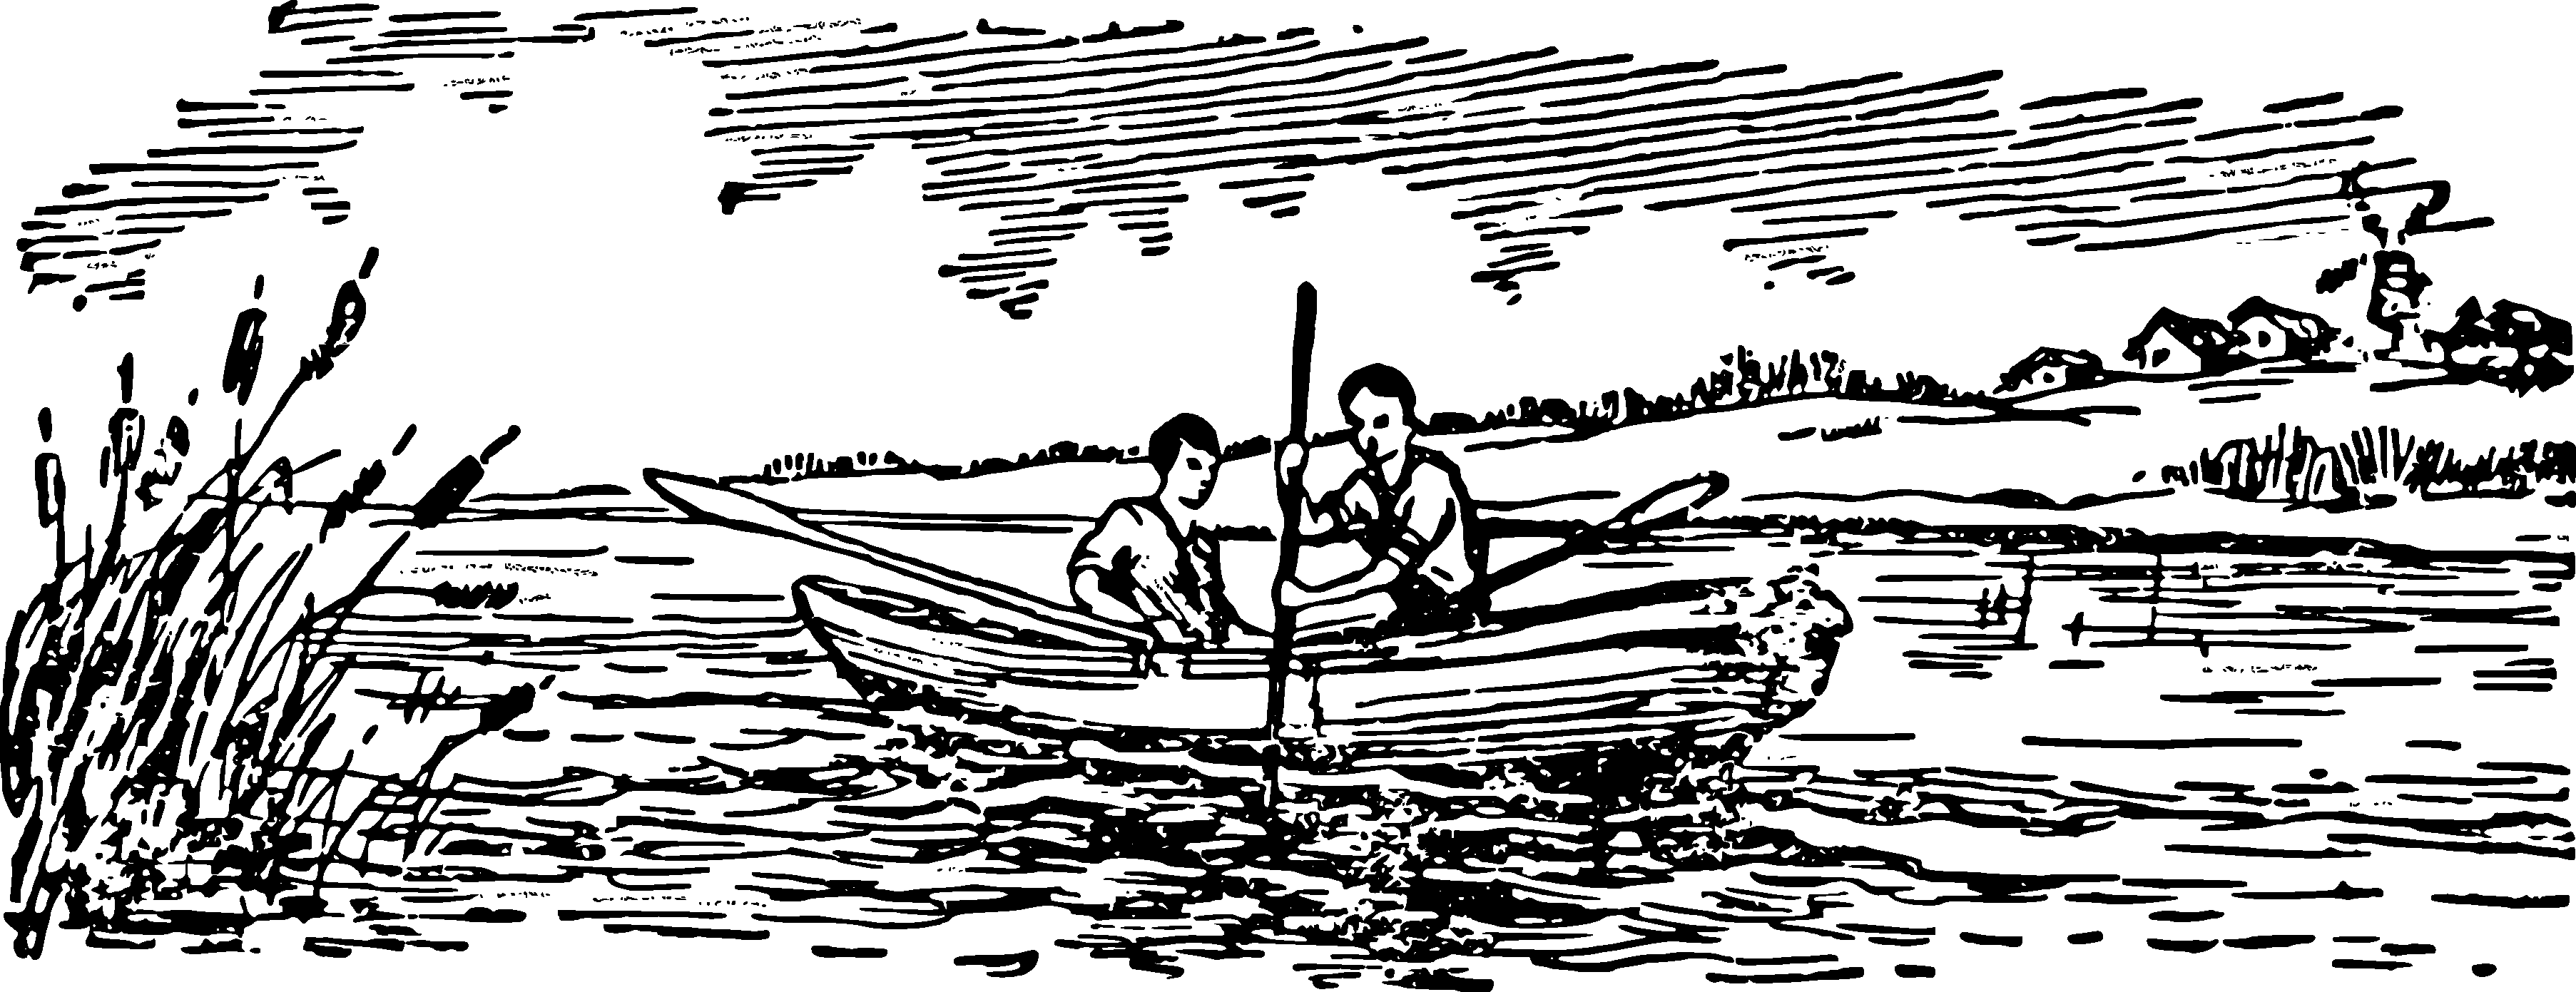
\includegraphics[width=1.2\textwidth]{figures/ch-02/fig-ch-02-head.pdf}\bigskip}

\chapter{Geometry By The River}
\label{ch-02}

\section{Measuring the width of the river}
\label{sec-2.1}
When crossing a river, measuring its width is just as easy for those who know geometry, how to determine the height of a tree, without climbing to the top. The inaccessible distance is measured the same techniques that we used to measure the inaccessible height. In both cases, the definition of the desired distance is replaced an example of another distance that is easily measurable directly.

Of the many ways to solve this problem, let's look at some of the simplest ones.

\begin{figure}[h!]
\centering
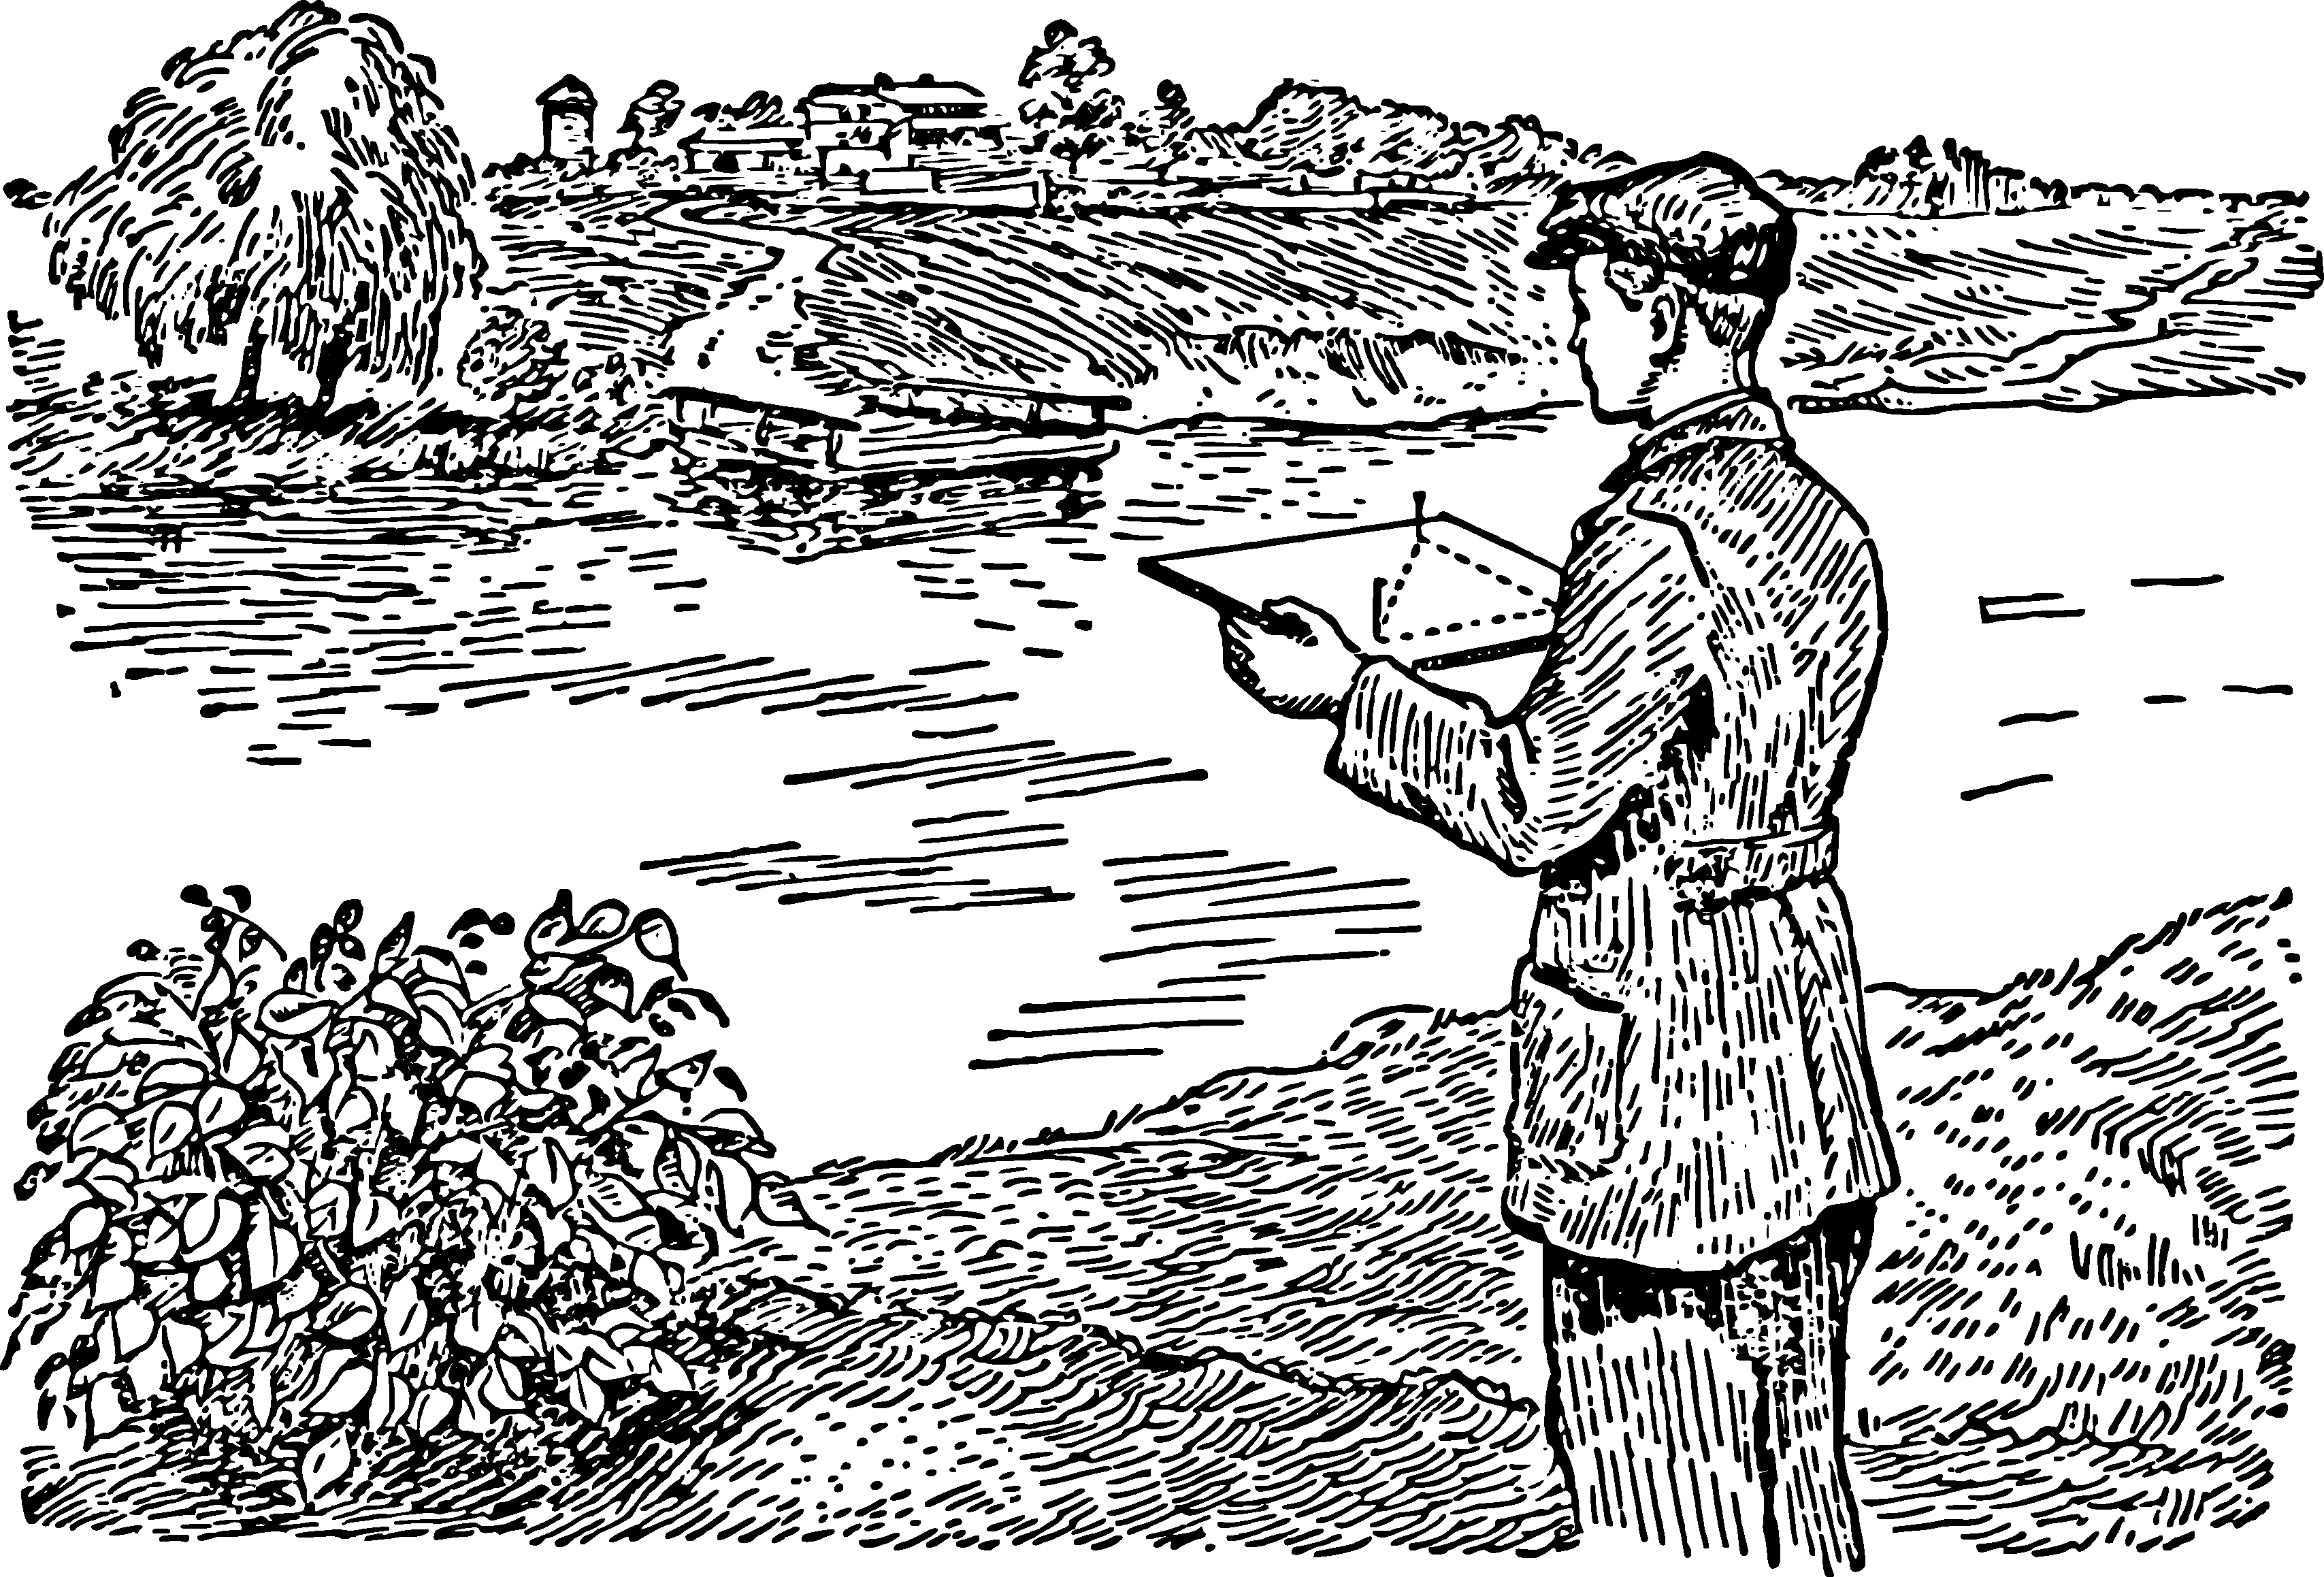
\includegraphics[width=0.9\textwidth]{figures/ch-02/fig-025.pdf}
\sidecaption{Measuring the width of the river with a pin device.\label{fig-025}}
\end{figure}

\begin{enumerate}
\item The first method requires the familiar ``device'' with three pins at the vertices of an isosceles right triangle (\figr{fig-025}). 
Let's say we need to determine the width of river $AB$ (\figr{fig-026}), standing on the bank where point $B$ is, without crossing to the opposite bank. Standing somewhere at point $C$, hold the pin device close to your eye so that, looking with one eye along the two pins, you see both covering points $B$ and $A$. It's clear that when you manage this, you will be exactly on the extension of line $AB$. 

\begin{marginfigure}[-1.5cm]%[h!]
\centering
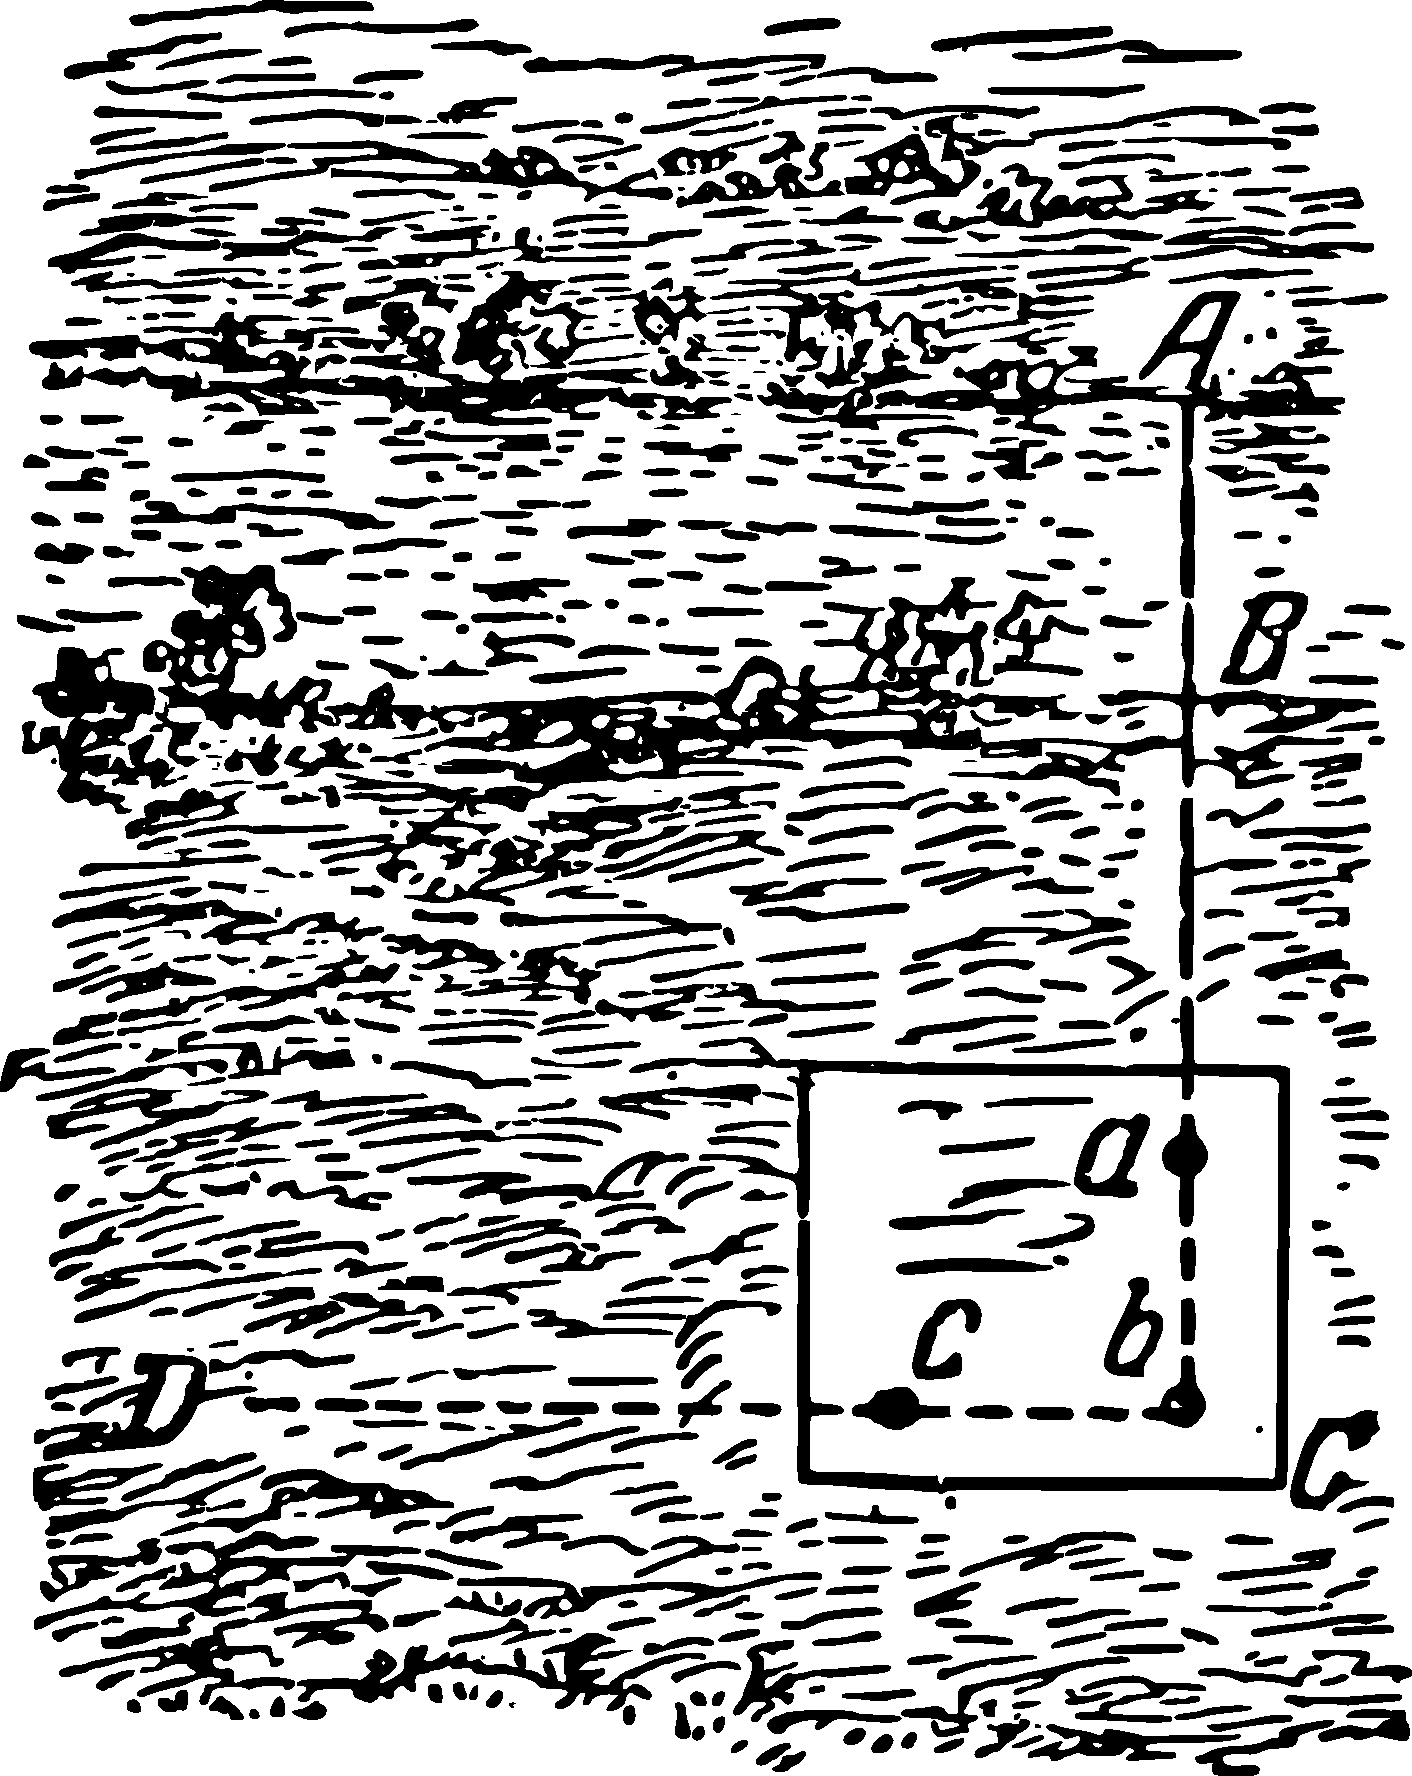
\includegraphics[width=\textwidth]{figures/ch-02/fig-026.pdf}
\sidecaption{First position of the pin device.\label{fig-026}}
\end{marginfigure}
\begin{marginfigure}[5cm]%[h!]
\centering
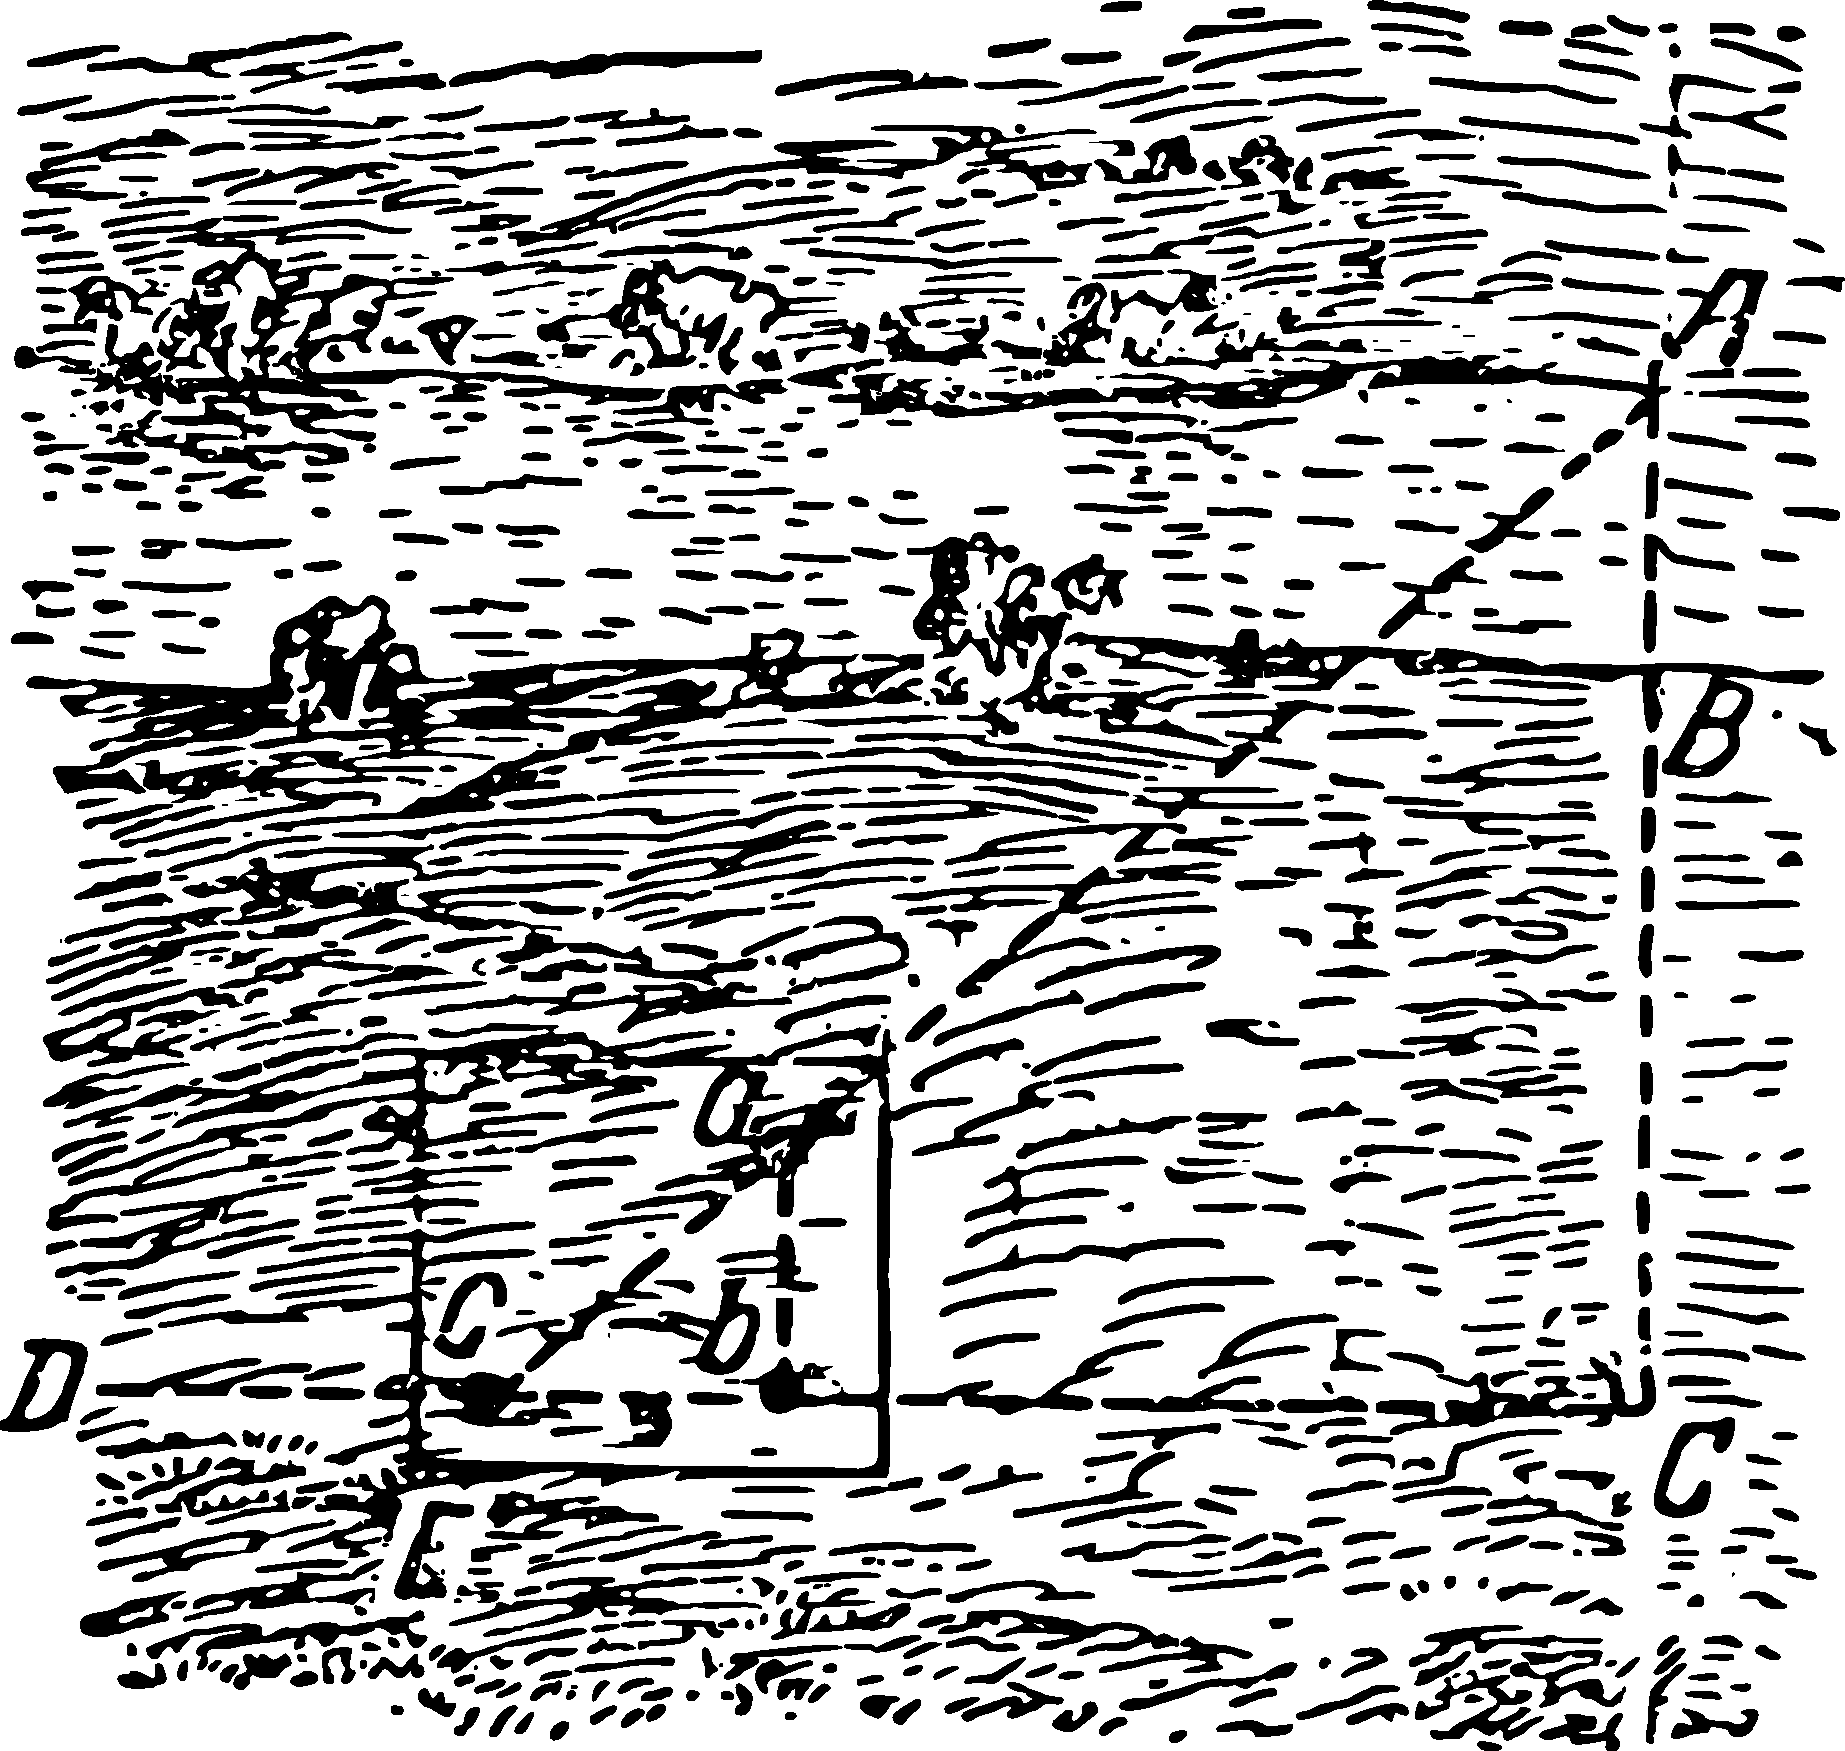
\includegraphics[width=\textwidth]{figures/ch-02/fig-027.pdf}
\sidecaption{Second position of the pin device.\label{fig-027}}
\end{marginfigure}


Now, without moving the plank of the device, look along the other two pins (perpendicular to the previous direction) and notice any point $D$ covered by these pins, i.e., lying on the line perpendicular to $AC$. After this, insert a pin at point $C$, leave this place, and go with your instrument along line $CD$ until you find a point $E$ (\figr{fig-027}), where you can simultaneously cover point $C$ for one eye with pin $b$ and point $A$ with pin $a$. This means you have found the third vertex of triangle $ACE$ on the shore, where angle $C$ is a right angle, and angle $E$ is opposite to the acute angle of the pin device, i.e., half the right angle (\ang{45}). Obviously, angle $A$ is also half right angle, i.e., $AC = CE$. If you measure the distance $CE$ even by steps, you will know the distance $AC$, and by subtracting $BC$, which is easy to measure, you will determine the desired width of the river.

It is quite inconvenient and difficult to hold the pin device still in hand; therefore, it is better to attach this plank to a stick with a pointed end and insert it vertically into the ground.

\item The second method is similar to the first. Here also, find point $C$ on the extension of $AB$ and mark line $CD$ perpendicular to $CA$ using the pin device. But then proceed differently (\figr{fig-028}). Equal distances $CE$ and $EF$ of arbitrary length are measured on the straight line $CD$, and pegs are inserted at points $E$ and $F$. Then, standing at point $F$ with a pin device, the direction $FG$ is marked out perpendicular to $FC$. Now, walking along $FG$, find a point $H$ on this line from which point $A$ seems to be covered by point $E$. This will mean that points $H$, $E$, and $A$ lie on the same straight line.

\begin{figure}[h!]
\centering
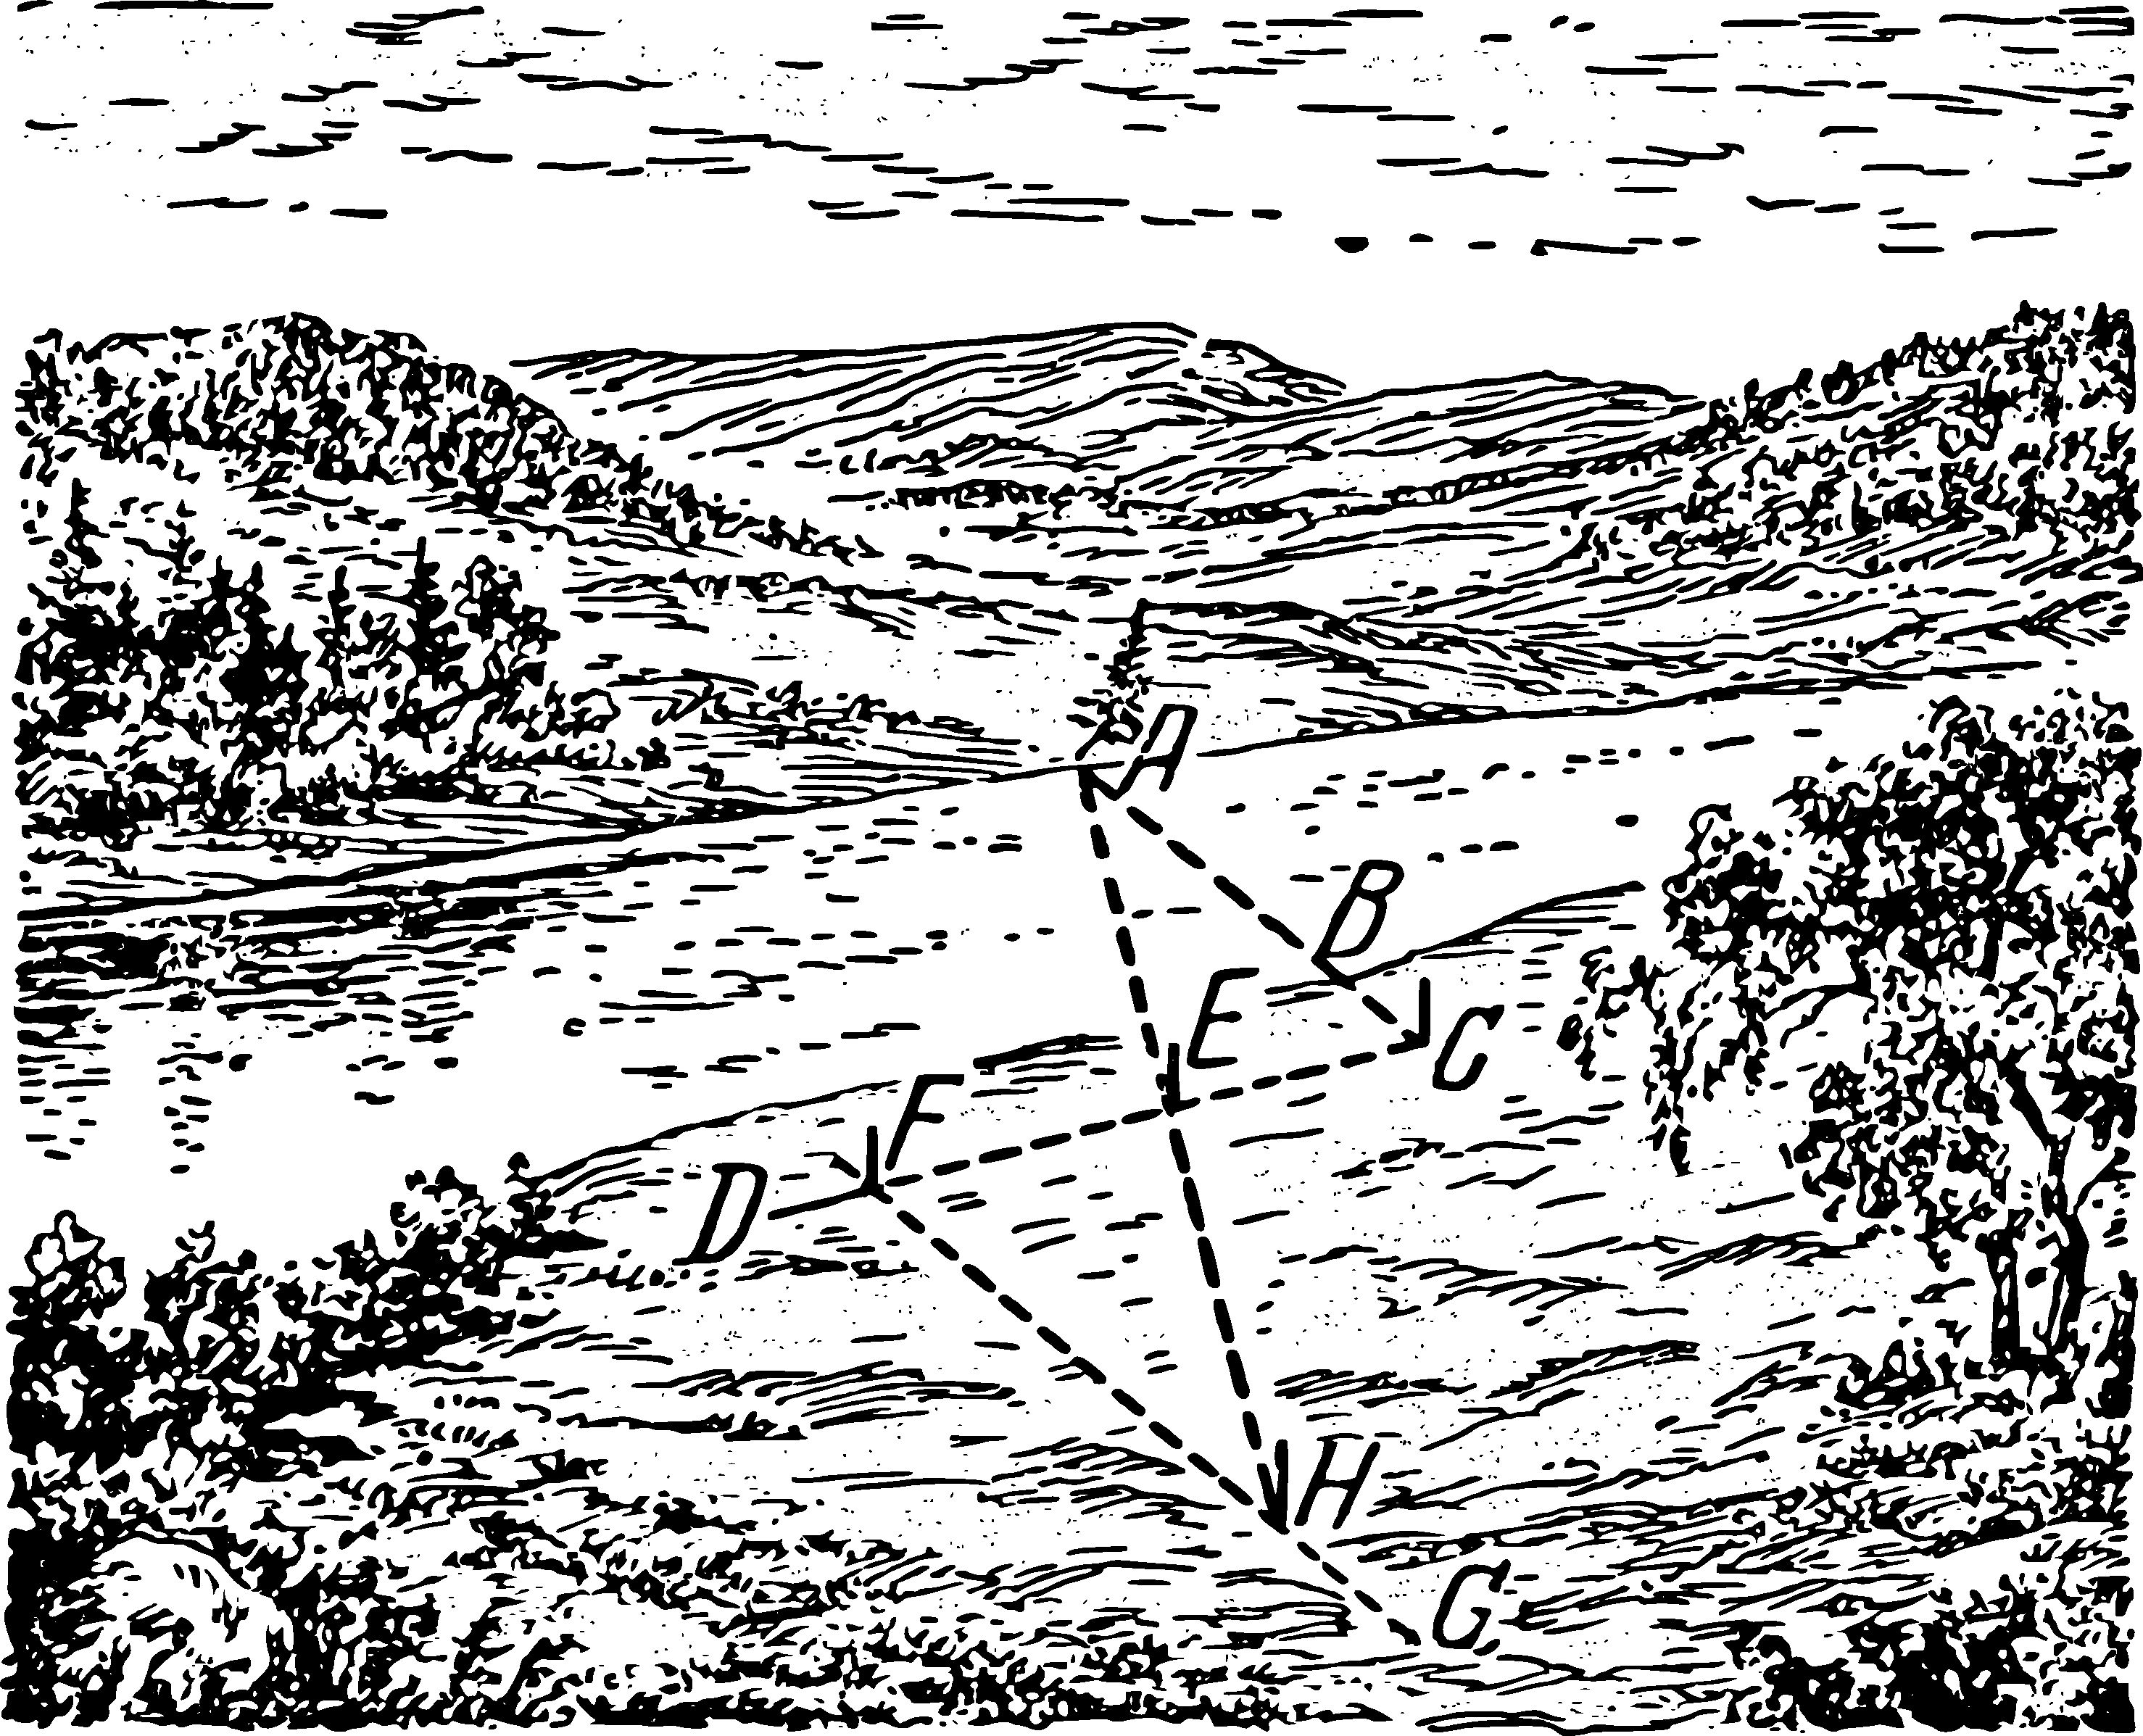
\includegraphics[width=0.9\textwidth]{figures/ch-02/fig-028.pdf}
\sidecaption{ Using the congruence criteria of triangles to find the width of the river.\label{fig-028}}
\end{figure}

The problem is solved: the distance $FH$ is equal to the distance $AC$, from which it is only necessary to subtract $BC$ to find the desired width of the river (the reader, of course, will guess for himself why $FH$ is equal to $AC$).

This method requires more space than the first one; if the terrain allows executing both methods, it is useful to verify one result by another.
\begin{figure}[h!]
\centering
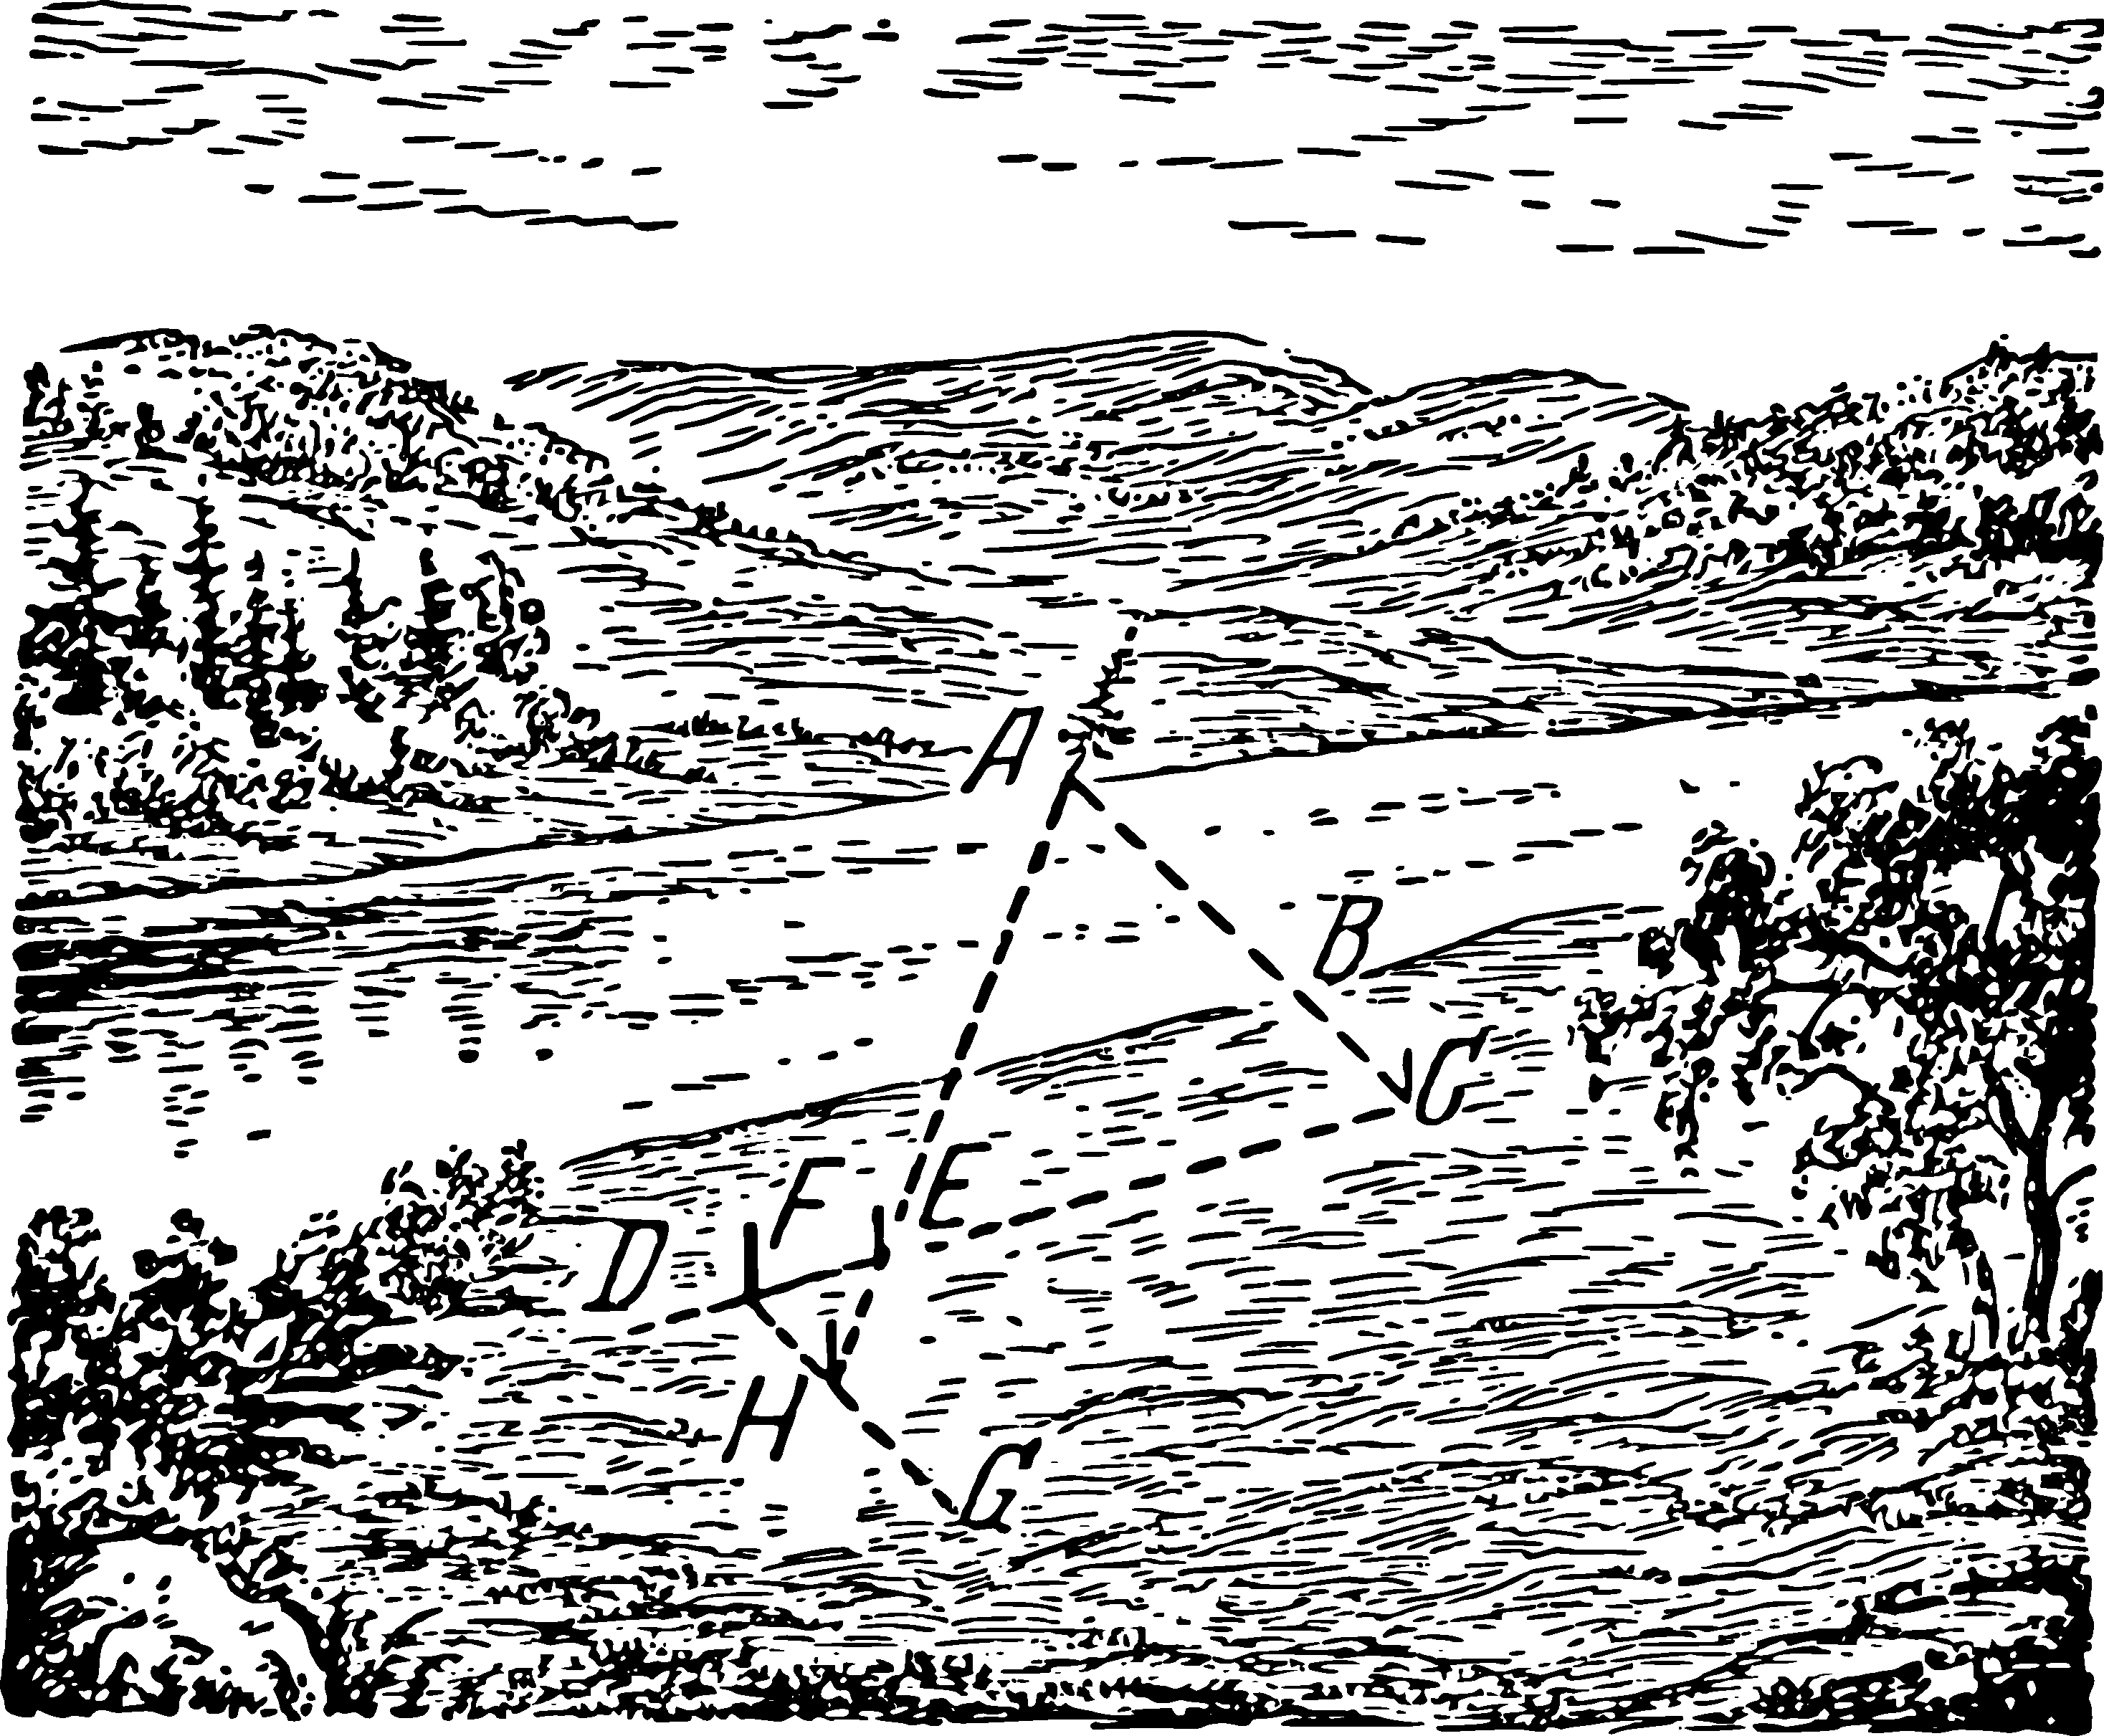
\includegraphics[width=0.9\textwidth]{figures/ch-02/fig-029.pdf}
\sidecaption{Using the similarity criteria of triangles to find the width of the river.\label{fig-029}}
\end{figure}

\item The method described above can be modified: instead of measuring equal distances on the straight line $CF$, measure one distance several times smaller than the other. For example (\figr{fig-029}), $FE$ is measured four times less than $EC$, and then we proceed as before: in the direction $FG$, perpendicular to $FC$, we find a point $H$ from which the peg $E$ appears to cover point $A$. But now $FH$ is no longer equal to $AC$, but four times smaller than this distance: triangles $ACE$ and $EFH$ are not congruent here, but similar (they have equal angles with unequal sides). From the similarity of triangles follows the proportion:
\begin{equation*}%
\frac{AC}{FH} = \frac{CE}{EF} = \frac{4}{1}
\end{equation*}
Therefore, by measuring $FH$ and multiplying the result by 4, we get the distance $AC$, and by subtracting $BC$, we find the desired width of the river.

This method, as we can see, requires less space and is therefore more convenient to perform than the previous one.




\item The fourth method is based on the property of a right triangle that if one of its acute angles is \ang{30}, then the length of the cathetus is half the hypotenuse. It is very easy to verify the correctness of this. 

Let angle $B$ of right triangle $ABC$ (\figr{fig-030}, left) be \ang{30}; we will prove that in this case, $AC = \nicefrac{1}{2}\, AB$. Rotate triangle $ABC$ around $BC$ so that it is symmetric with its initial position (\figr{fig-030}, right), forming figure $ABD$; line $AC$ is straight because both angles at point $C$ are right angles. In triangle $ABD$, angle $\angle A = \ang{60}$, angle $ABD$, composed of two \ang{30} angles, is also equal to \ang{60}. Therefore, $AD = BD$ as sides opposite equal angles. But $AC = \nicefrac{1}{2} \,AD$, therefore,
\begin{marginfigure}[-3cm]%[h!]
\centering
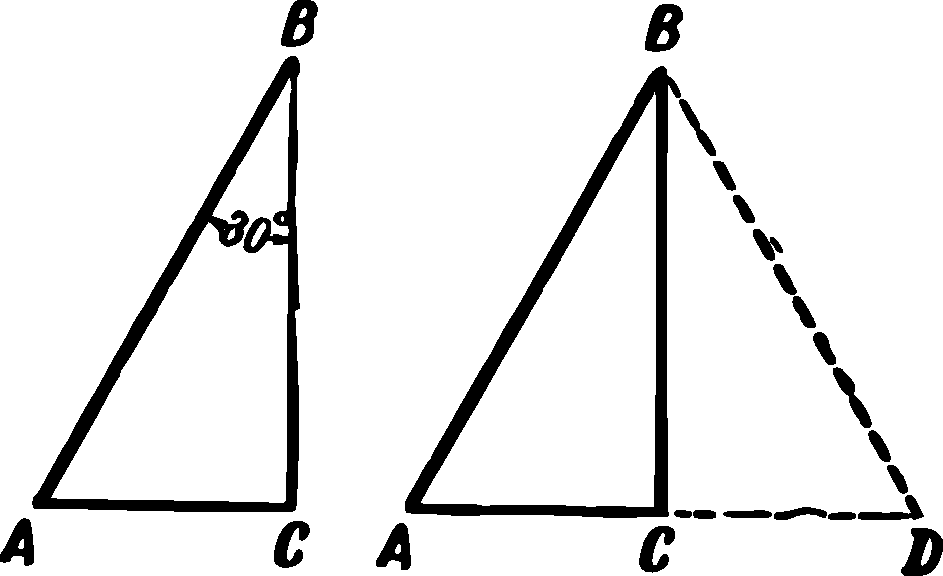
\includegraphics[width=\textwidth]{figures/ch-02/fig-030.pdf}
\sidecaption{When the cathetus is half the hypotenuse.\label{fig-030}}
\end{marginfigure}
\begin{equation*}%
AC = \frac{1}{2} AB.
\end{equation*}
Wishing to take advantage of this property of the triangle, we must arrange the pins on the board so that their bases represent a right triangle in which the cathetus is half the hypotenuse. With this device, we place ourselves at point $C$ (\figr{fig-031}) so that the direction $AC$ coincides with the hypotenuse of the pin triangle. 
\begin{marginfigure}[-2cm]%[h!]
\centering
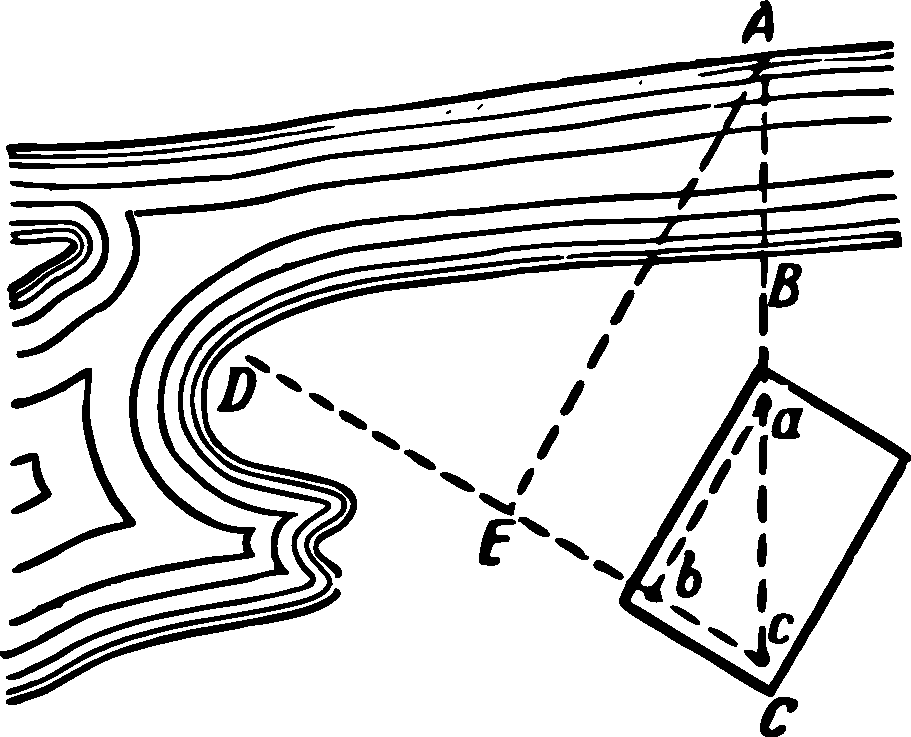
\includegraphics[width=\textwidth]{figures/ch-02/fig-031.pdf}
\sidecaption{The scheme of application of a right-angled triangle with a 30° angle.\label{fig-031}}
\end{marginfigure}
Looking along the short cathetus of this triangle, mark the direction $CD$ and find a point $E$ on it so that the direction $EA$ is perpendicular to $CD$ (this is done using the same pin device). It is easy to see that the distance $CE$ -- the cathetus lying opposite the angle of \ang{30} -- is equal to half of $AC$. Therefore, by measuring $CE$, doubling this distance and subtracting $BC$, we obtain the desired width of the $AB$ river.

\end{enumerate}

Here are four easily executable methods, with which it is always possible, without crossing to the other bank, to measure the width of the river with quite satisfactory accuracy. We will not consider methods that require the use of more complex instruments (even homemade ones) here.

\section{Using a visor}
\label{sec-2.2}

Here's how this method came in handy for Senior Sergeant Kupriyanov in frosty conditions.\sidenote{See the footnote on page~\pageref{ref-21}.} His detachment was ordered to measure the width of the river, across which they were to organise a crossing\ldots{}

Approaching a bush near the river, Kupriyanov's detachment took cover, and Kupriyanov himself, along with soldier Karpov, moved closer to the riverbank, from where the fascist-occupied shore was clearly visible. In such conditions, measuring the width of the river had to be done by eye.

``Come on, Karpov, how much?'' Kupriyanov asked.

``I think no more than 100-110 meters,'' Karpov replied. Kupriyanov agreed with his scout, but for control, he decided to measure the width of the river using a ``visor.''

\begin{figure}[h!]
\centering
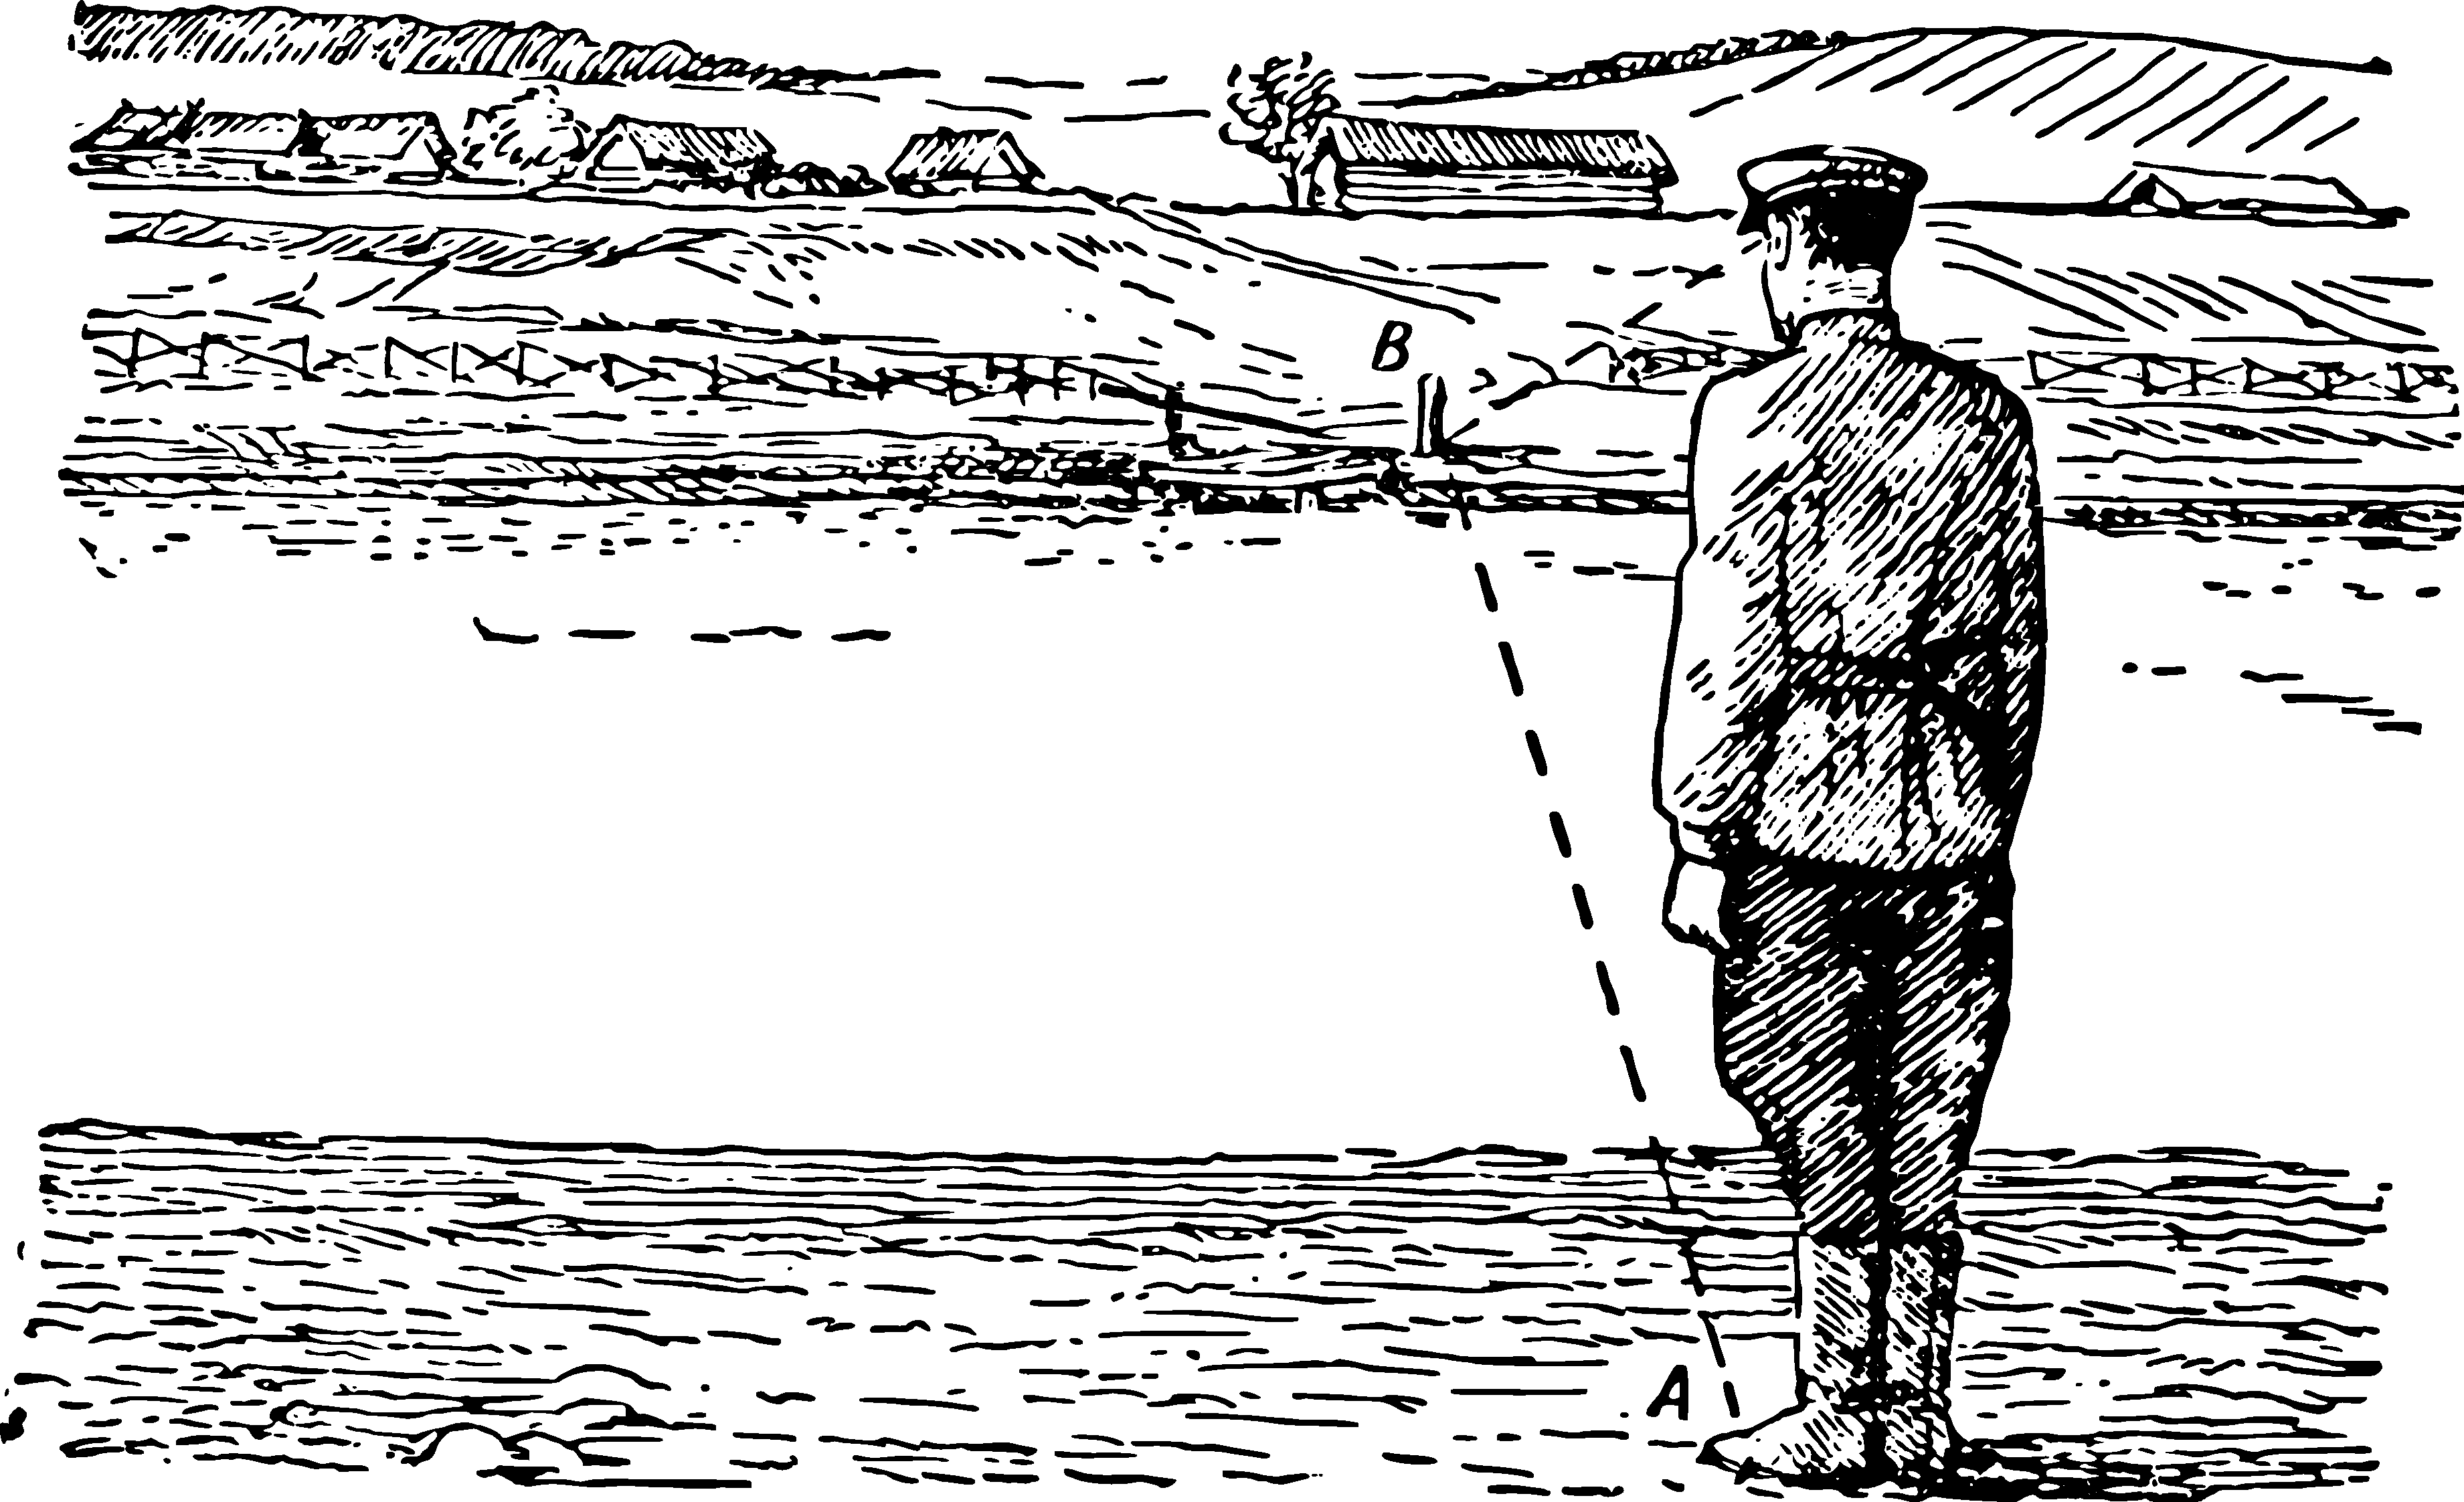
\includegraphics[width=0.9\textwidth]{figures/ch-02/fig-032.pdf}
\sidecaption{Observing a point on the opposite bank from under the visor.\label{fig-032}}
\end{figure}

This method is simple. You have to face the river and pull the visor over your eyes so that the lower edge of the visor precisely aligns with the line of the opposite bank (see \figr{fig-032}). The visor can be replaced with the palm of your hand or a notepad, tightly pressed edge to your forehead. Then, without changing the position of your head, you need to turn to the right or left, or even backward (towards the side where the area available for measuring the distance is more level) and notice the farthest point visible from under the visor (palm, notepad).

The distance to this point will be approximately equal to the width of the river.

Kupriyanov utilized this method. He quickly stood up in the bushes, pressed a notepad to his forehead, then quickly turned and aimed at the distant point. Then, together with Karpov, he crawled to that point, measuring the distance with a rope. It turned out to be 105 meters.

Kupriyanov reported the data he obtained to the command.

\ques Provide a geometric explanation for the ``visor'' method.

\begin{figure}[h!]
\centering
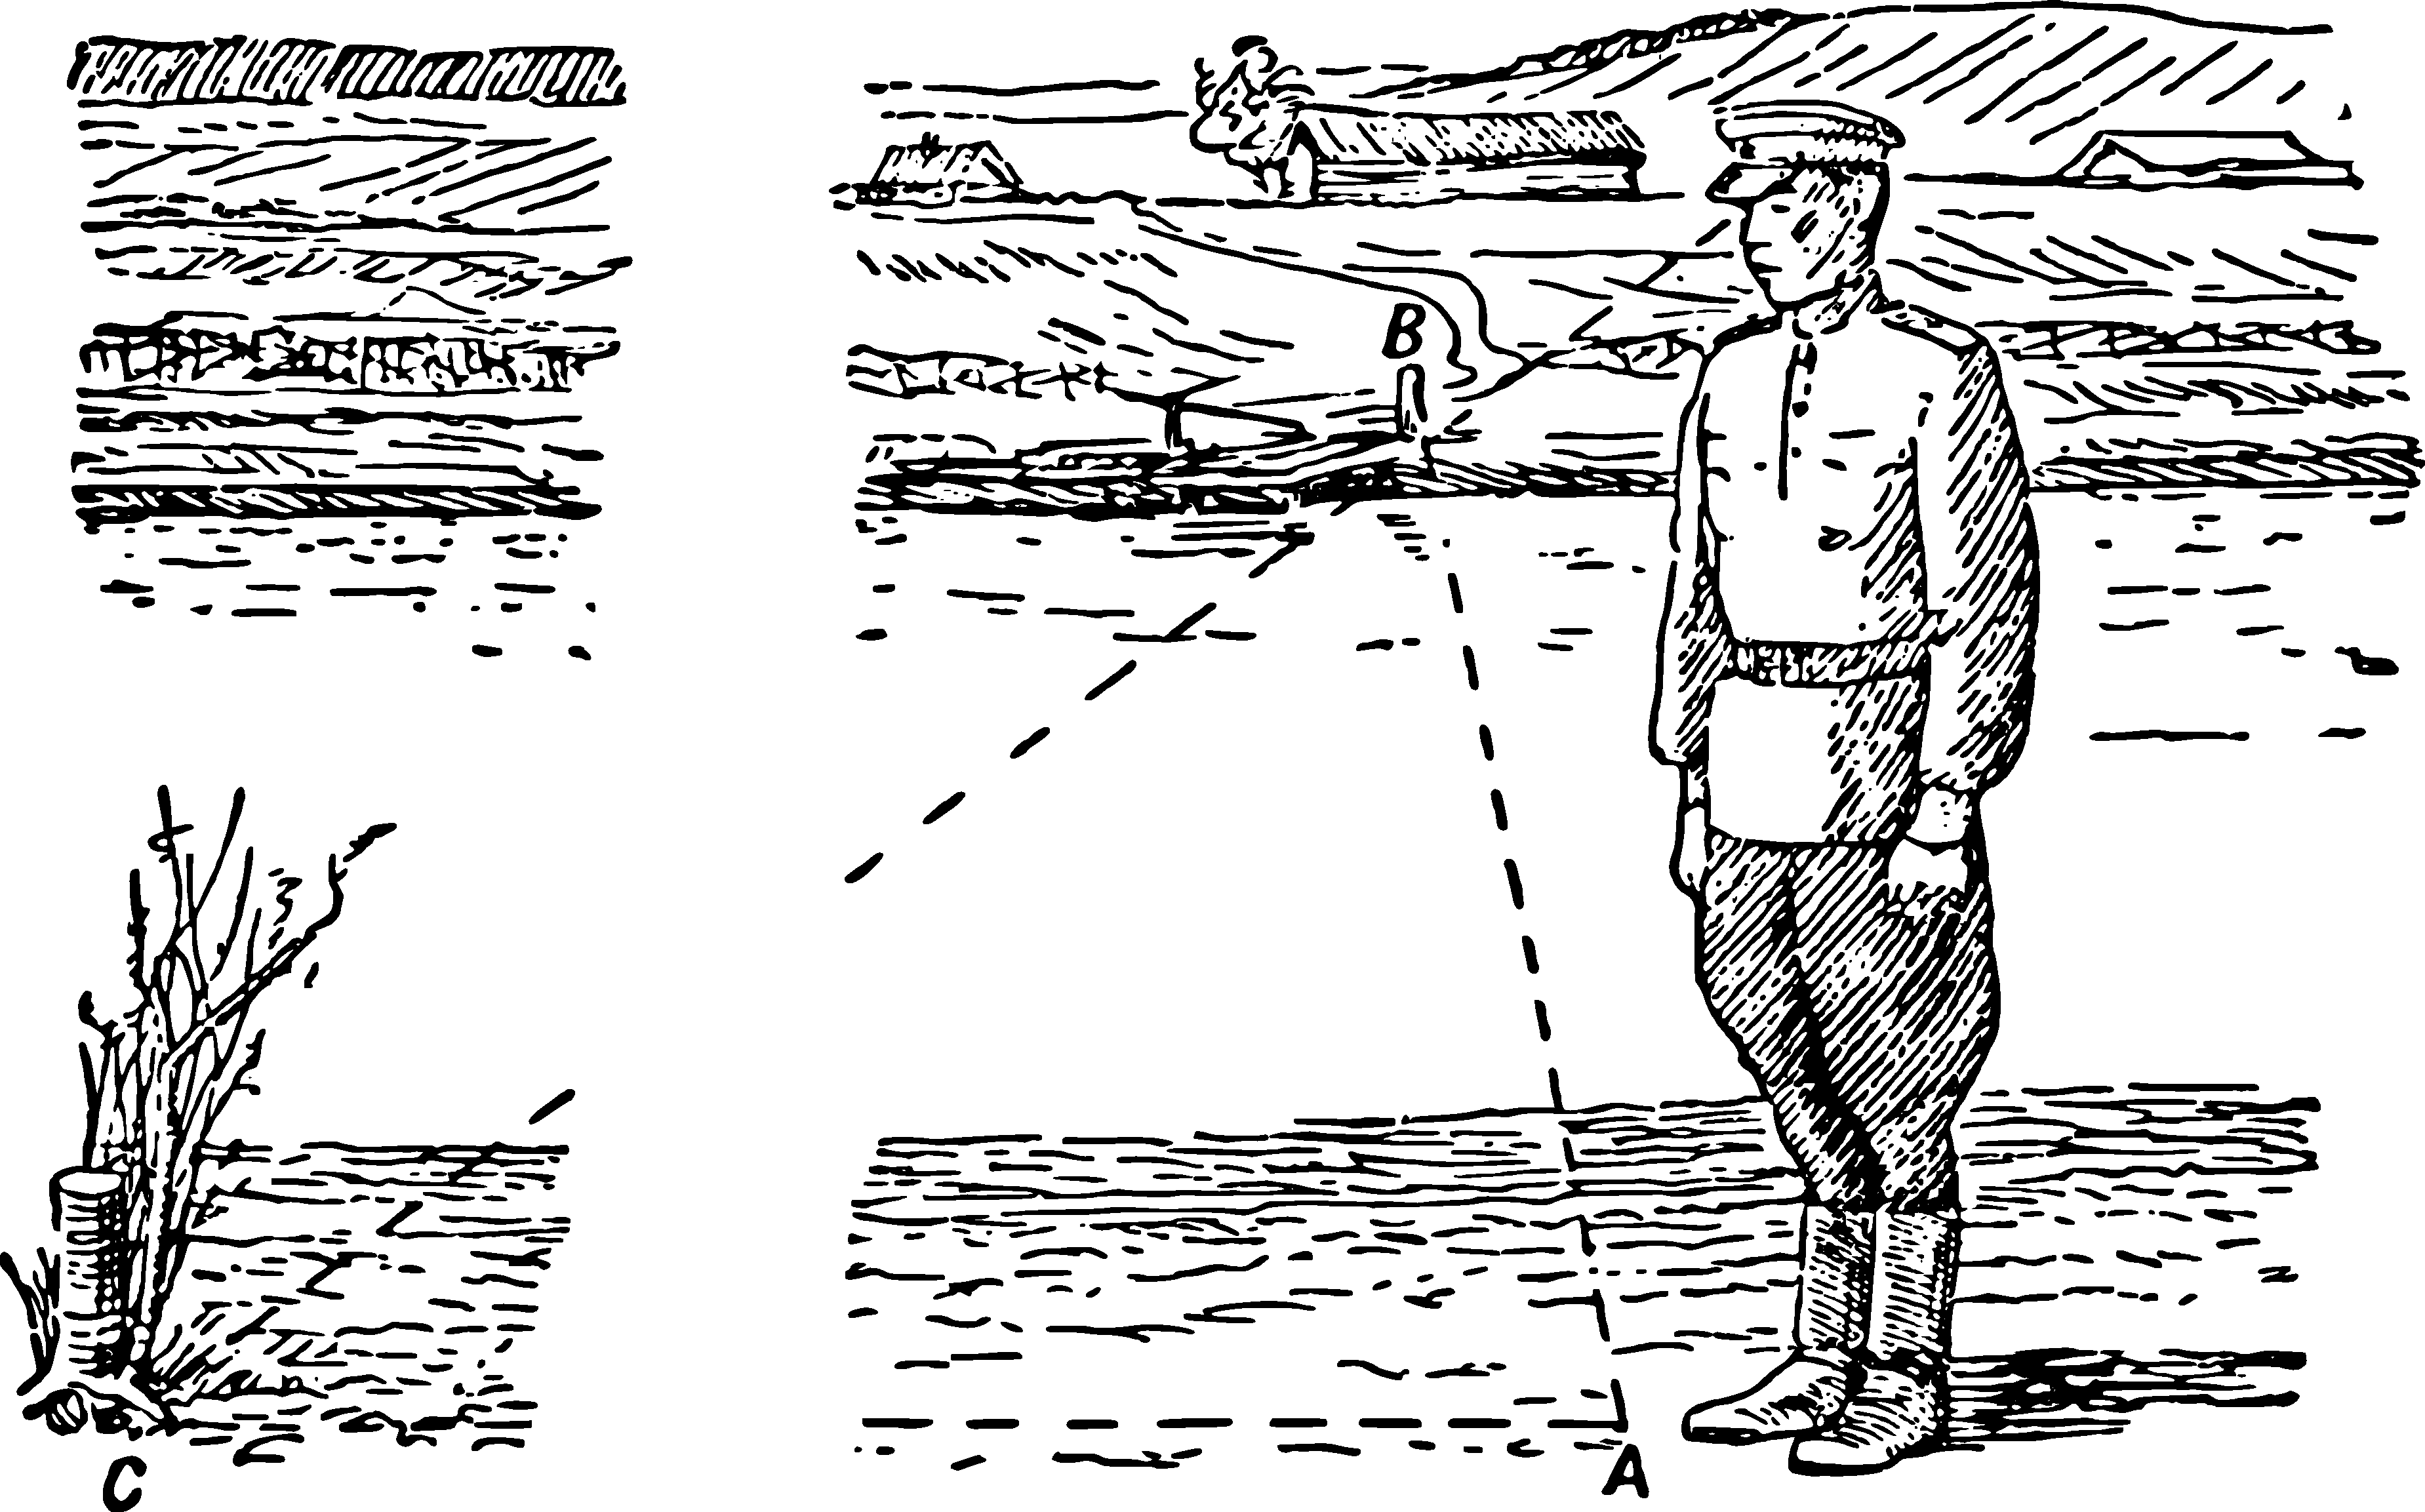
\includegraphics[width=0.9\textwidth]{figures/ch-02/fig-033.pdf}
\sidecaption{In the same way, you can aim at a point on your own bank.\label{fig-033}}
\end{figure}

\ans The line of sight, touching the edge of the visor (palm, notepad), is initially directed towards the line of the opposite bank (see \figr{fig-032}). When a person turns, the line of sight, like the leg of a compass, describes a circle, and then $AC = AB$ as the radii of the same circle (see \figr{fig-033}). 

\section{The Length Of An Island}

\ques Now we are faced with a more challenging task. Standing by the river or lake, you see an island (see \figr{fig-034}) whose length you wish to measure without leaving the shore. Is it possible to carry out such a measurement?

Although in this case, both ends of the measured line are inaccessible to us, the problem is still entirely solvable, and without complex instruments.

\begin{figure}[h!]
\centering
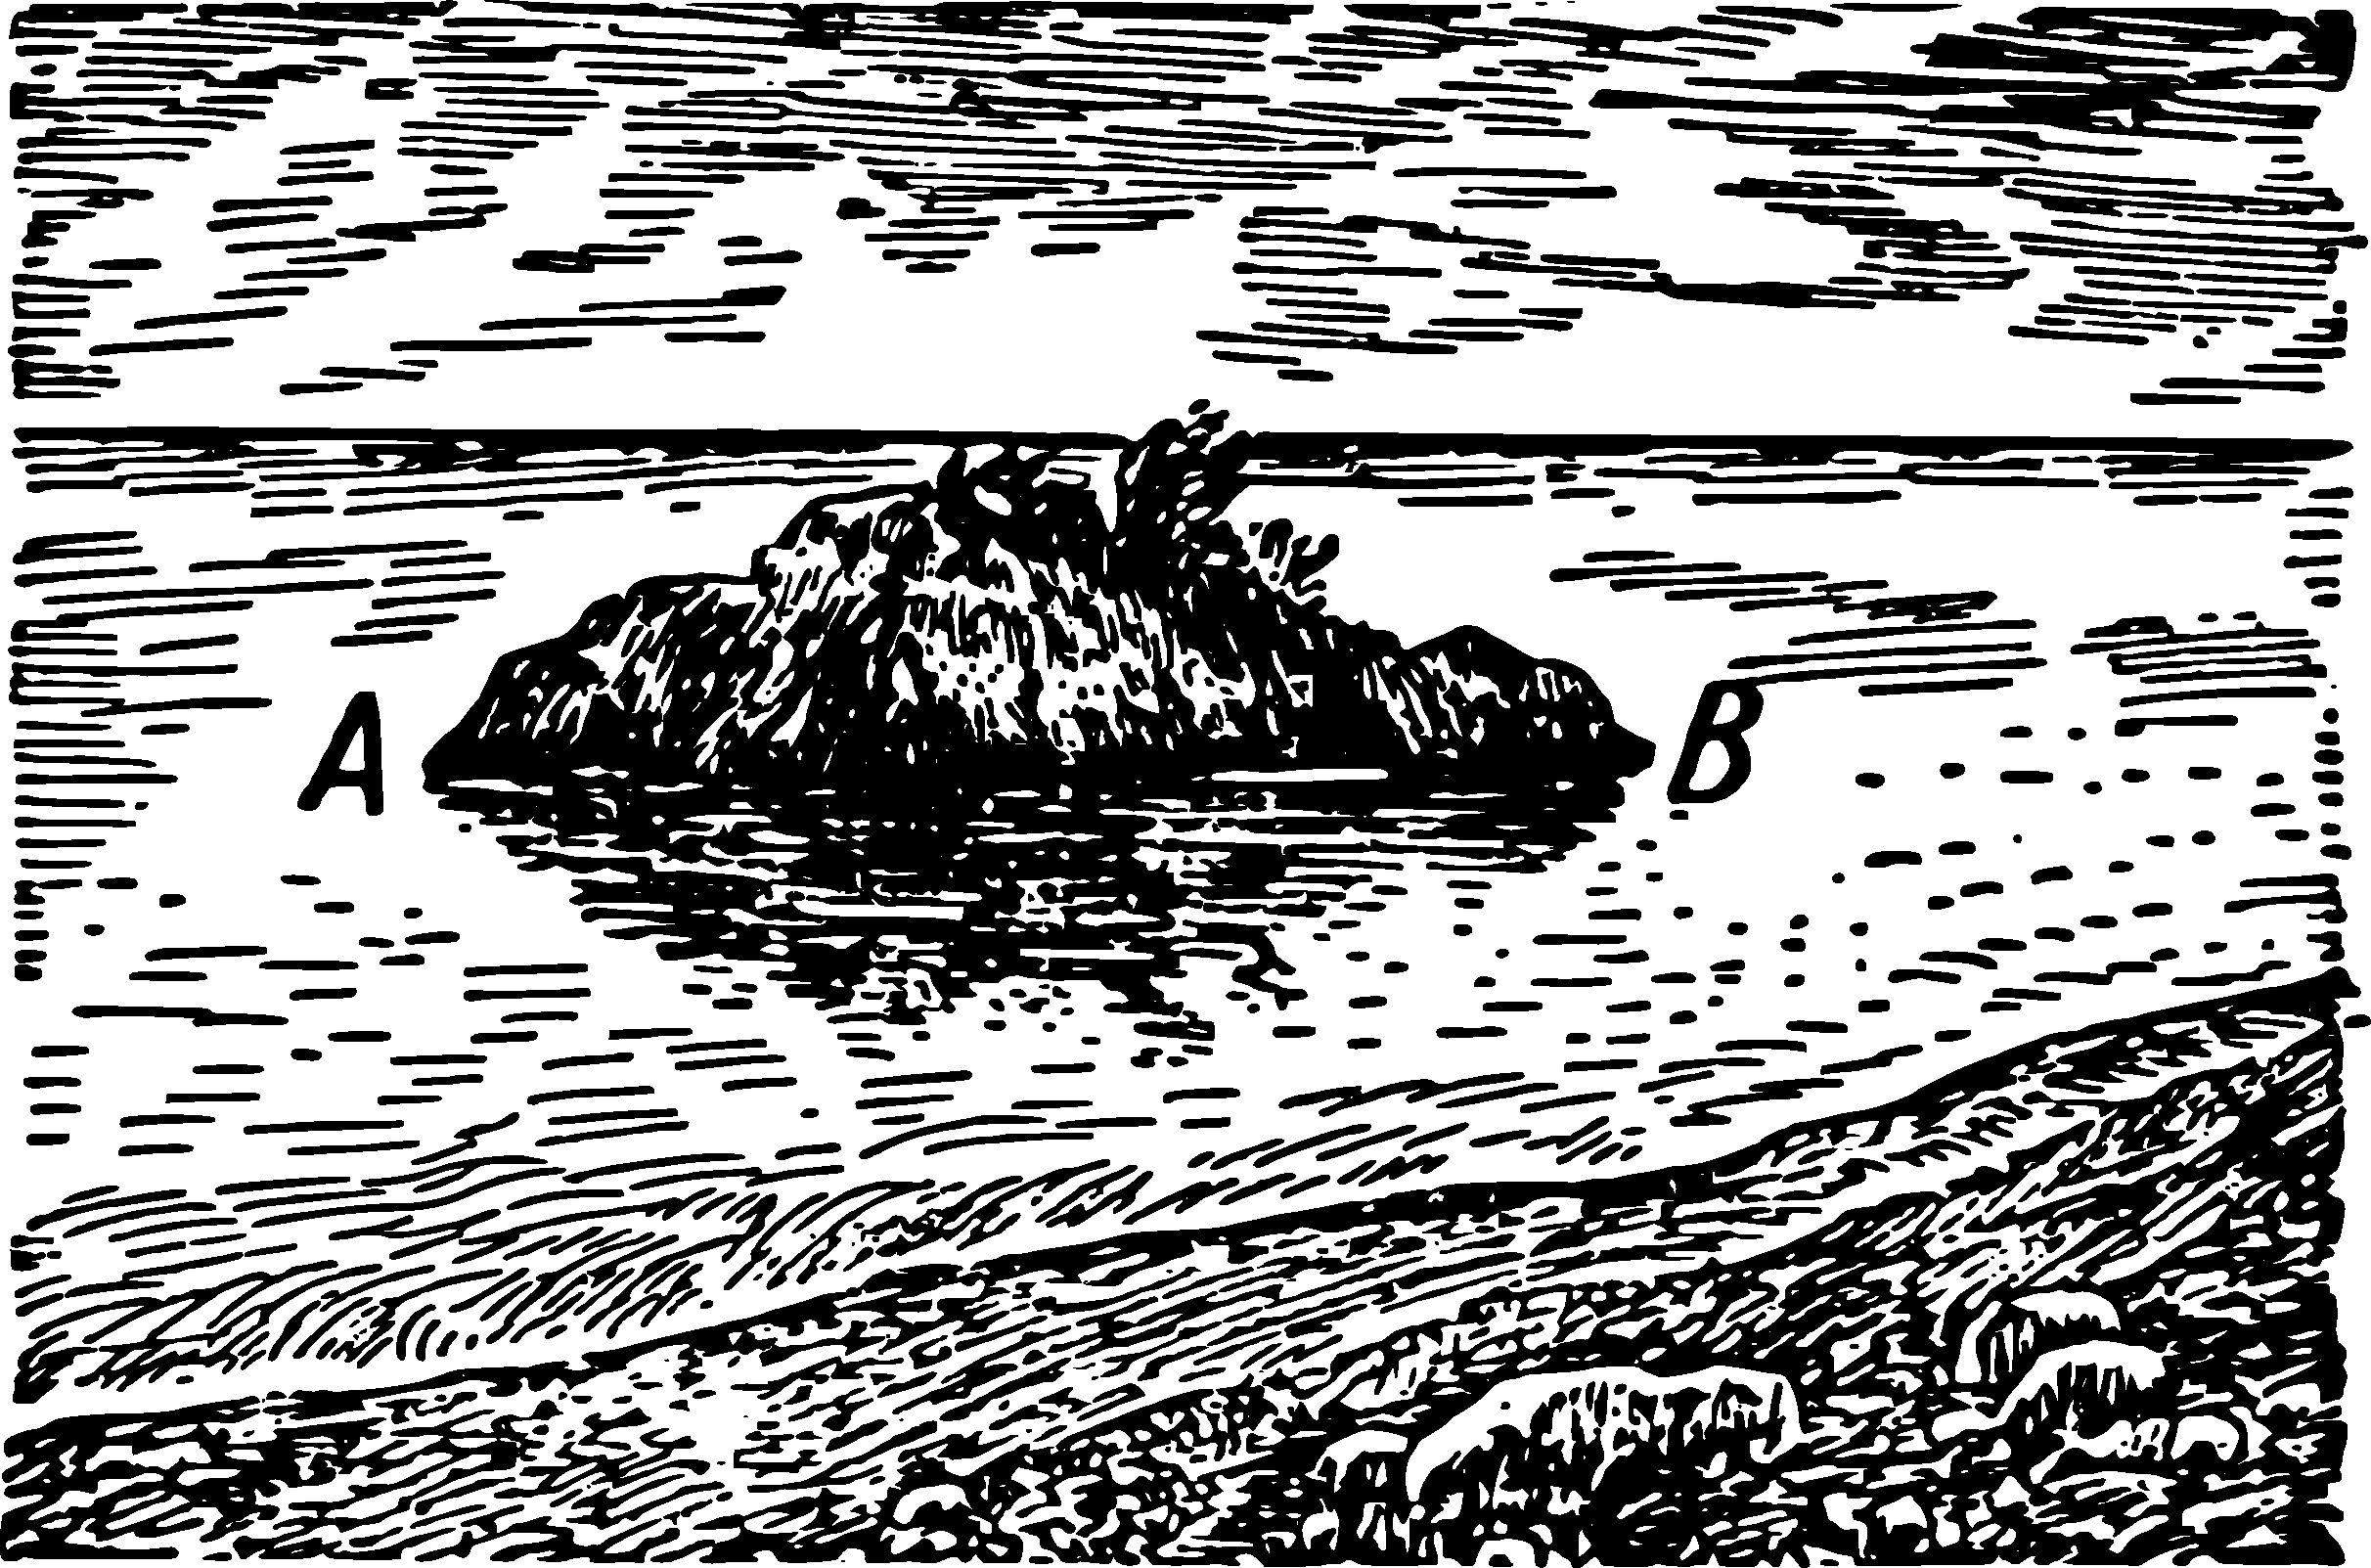
\includegraphics[width=0.9\textwidth]{figures/ch-02/fig-034.pdf}
\sidecaption{How to determine the length of the island.\label{fig-034}}
\end{figure}


\ans To measure the length of an island without leaving the shore, you can use the following method. Choose arbitrary points $P$ and $Q$ on the shore and place stakes in them. Then find points $M$ and $N$ on the line $PQ$ such that the directions $AM$ and $BM$ form right angles with the direction of $PQ$ (this can be done using a compass). In the middle of the distance $MN$, place a stake $O$ and find on the extension of the line $AM$ a point $C$ from which the stake $O$ appears to cover point $B$. Similarly, on the extension of $BN$, find point $D$ from which stake $O$ appears to cover the end $A$ of the island. The distance $CD$ will be the desired length of the island.

\begin{marginfigure}[-3cm]%[h!]
\centering
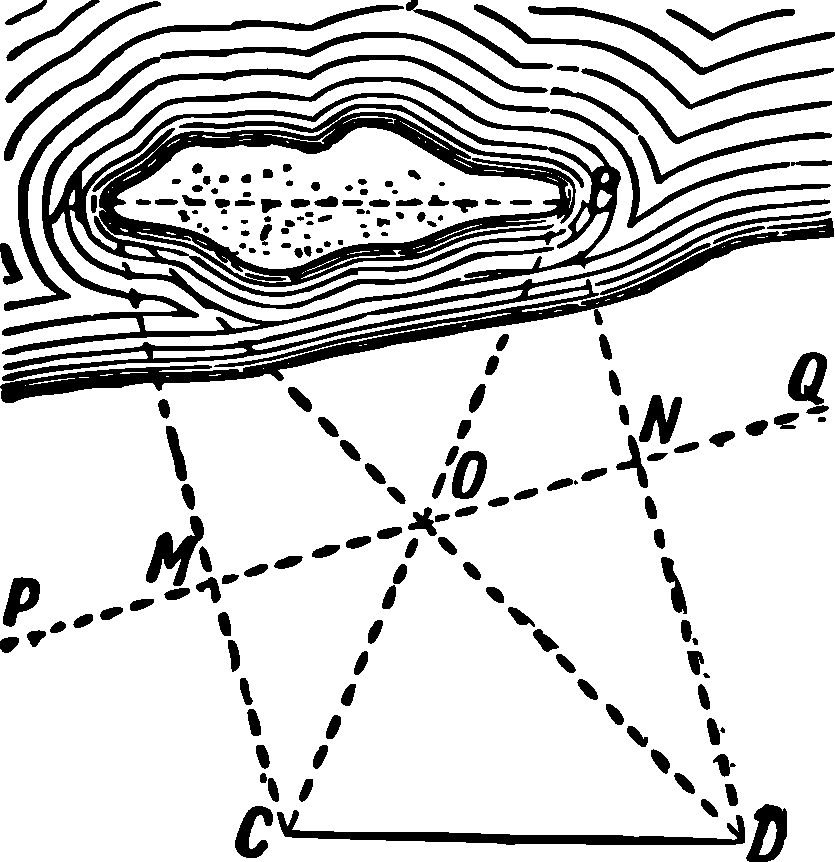
\includegraphics[width=\textwidth]{figures/ch-02/fig-035.pdf}
\sidecaption{We use the properties of congruent right triangles to find the length of an isalnd.\label{fig-035}}
\end{marginfigure}

This can be easily proved. Consider the right triangles $AMO$ and $OND$; in them, the legs $MO$ and $NO$ are equal, and the angles $AOM$ and $NOD$ are also equal, therefore, the triangles are equal, and $AO = OD$. Similarly, it can be proved that $BO = OC$. By comparing the triangles $ABO$ and $COD$, it can be seen that their distances $AB$ and $CD$ are equal.

\section{A pedestrian on the opposite bank}
\label{sec-2.3}

\ques As you walk along the riverbank, you see a person on the other side, and you can clearly distinguish their steps. Can you, without moving from your spot, determine at least approximately the distance between them and you? You have no instruments at hand.

\begin{figure}[h!]
\centering
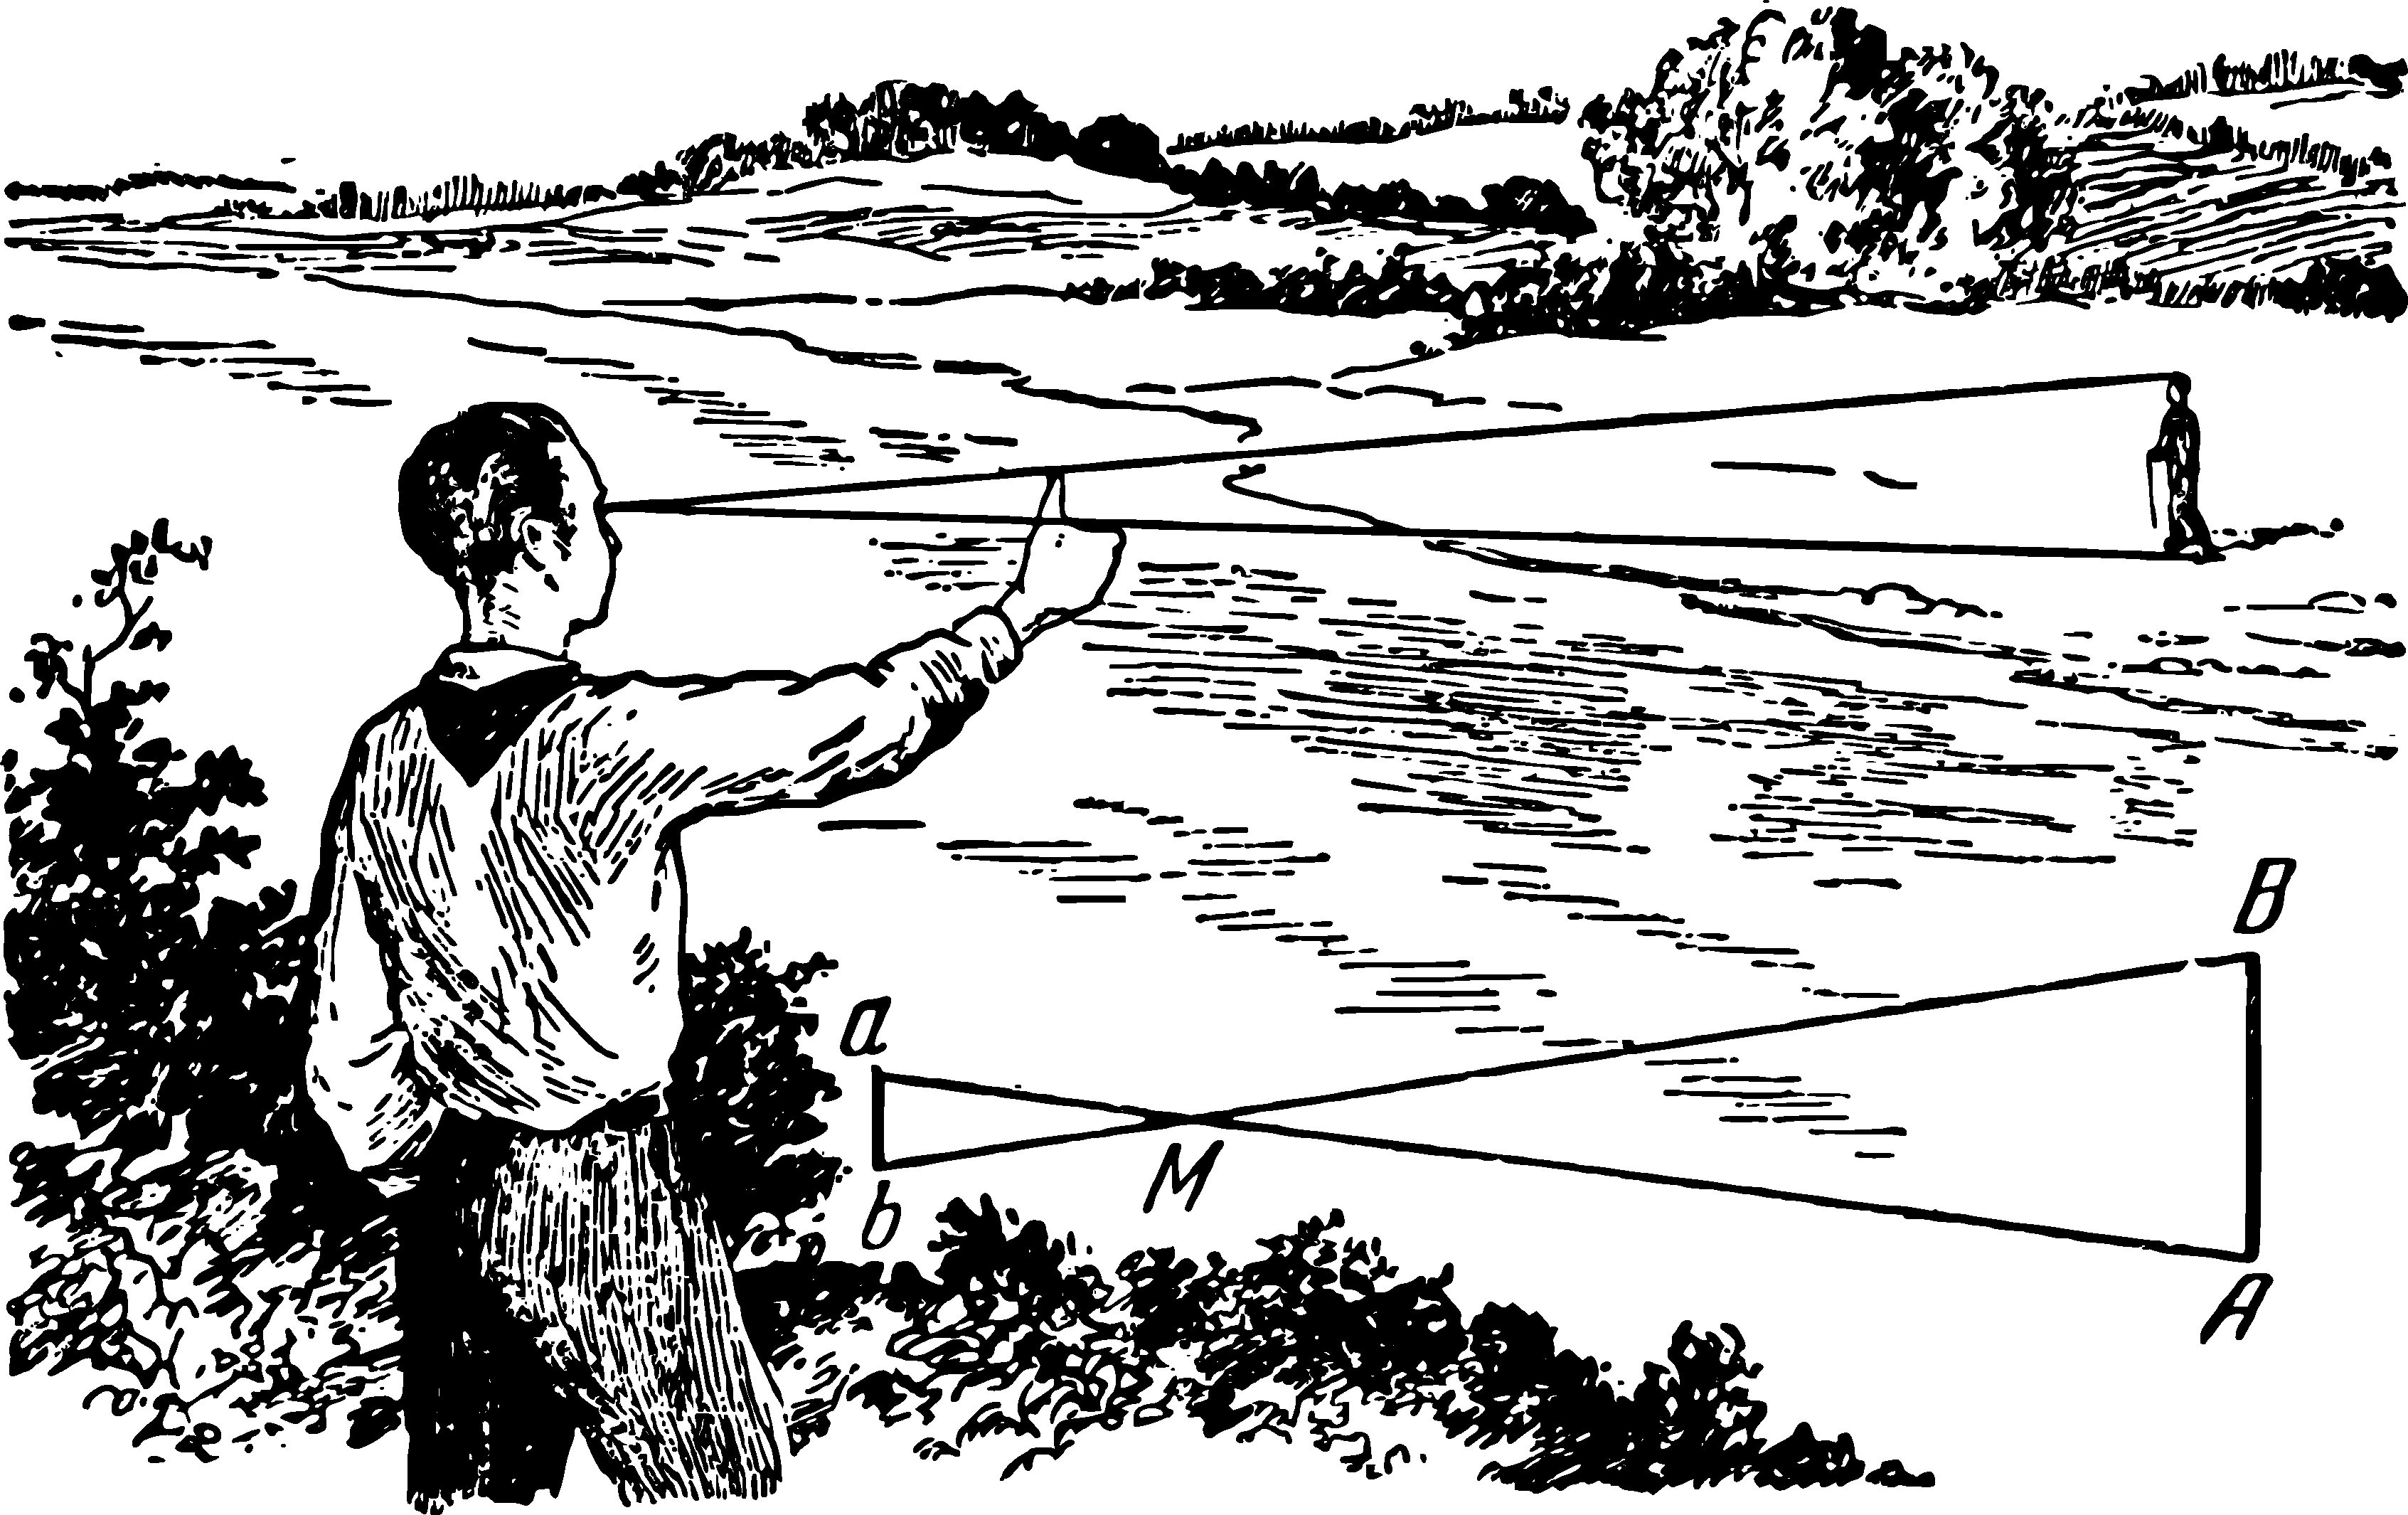
\includegraphics[width=0.9\textwidth]{figures/ch-02/fig-036.pdf}
\sidecaption{How to determine the distance to a pedestrian walking on the other side of the river.\label{fig-036}}
\end{figure}


\ans You don't have any instruments, but you have eyes and hands -- that's enough. Extend your arm forward towards the pedestrian and look at the tip of your finger with one eye if the pedestrian is moving towards your right hand, and with the other eye if they're moving towards your left hand. At the moment when the distant pedestrian is covered by your finger (see \figr{fig-036}), close the eye that was looking and open the other: the pedestrian will appear to you as if they've moved backward. Count how many steps they take before they align again with your finger. You'll get all the data needed for an approximate determination of the distance. Let's explain how to use them.

Suppose in \figr{fig-036} (inset), your eyes are marked as $a$ and $b$, point $M$ is the tip of your finger extended, point $A$ is the initial position of the pedestrian, and $B$ is the final position. The triangles $abM$ and $ABM$ are similar (you should turn towards the pedestrian so that $ab$ is approximately parallel to their direction of movement). Therefore, $BM : bM = AB : ab$ -- is a proportion in which only one term, $BM$, is unknown, but all others can be directly determined. Indeed, $bM$ is the length of your extended arm, $ab$ is the distance between the pupils of your eyes, and $AB$ is measured in steps taken by the pedestrian (assuming an average step to be around 3/4 metres). Therefore, the unknown distance from you to the pedestrian on the opposite bank, $AB$, equals 
\begin{equation*}%
MB = AB \, \frac{bM}{ab}
\end{equation*}
For example, if the distance between your eye pupils $ab$ is \SI{6}{\centi\meter}, the length of $bM$ from the end of your extended arm to the eye is \SI{60}{\centi\meter}, and the pedestrian takes, say, 14 steps from $A$ to $B$, then their distance from you would be $MB = 14 \cdot 60/6 = 140$ steps, or 105 meters.

It's enough for you to measure in advance the distance between your eye pupils and $bM$ -- the distance from the eye to the end of your extended arm -- so that you can quickly determine the distance of inaccessible objects by remembering their ratio. On average, for most people, $bM/ab$ is around 10 with slight fluctuations. The difficulty will only be in somehow determining the distance $AB$. In our case, we used the steps of a distant person. But you can also use other references. For instance, if you're measuring the distance to a distant freight train, you can estimate $AB$ in comparison to the length of a freight car, which is usually known (7.6 meters between buffers). If you're determining the distance to a house, you can estimate $AB$ by comparing it to the width of a window, the length of a brick, etc.

The same method can be applied to determine the size of a distant object if its distance from the observer is known. For this purpose, you can also use other ``rangefinders'', which we will describe next.

\section{Simple Rangefinders}
\begin{marginfigure}[-2cm]%[h!]
\centering
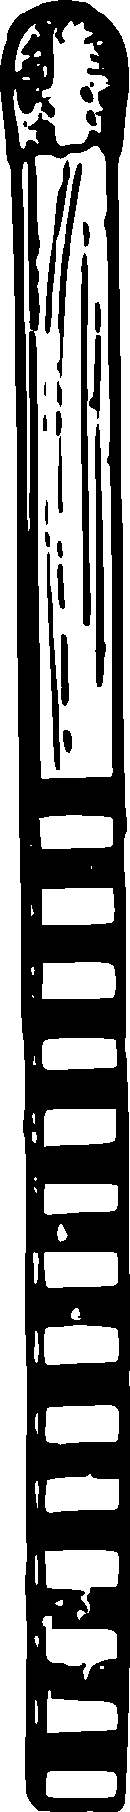
\includegraphics[width=0.1\textwidth]{figures/ch-02/fig-037.pdf}
\sidecaption{The match is a rangefinder.\label{fig-037}}
\end{marginfigure}
In the first chapter, we described the simplest instrument for determining inaccessible heights -- the altimeter. Now, let's describe the simplest device for measuring inaccessible distances -- the `rangefinder.' The simplest rangefinder can be made from an ordinary matchstick. To do this, you just need to mark millimeter divisions on one of its sides, alternating between light and dark (see \figr{fig-037}).


You can use this primitive ``rangefinder'' to estimate the distance to a distant object only in those cases when the dimensions of that object are known to you (see \figr{fig-038}). However, more sophisticated rangefinders can also be used under the same condition. Suppose you see a person in the distance and set yourself the task of determining the distance to them. Here, the matchstick rangefinder can come in handy. Holding it in your outstretched arm and looking with one eye, you bring its free end into coincidence with the top of the distant figure. Then, slowly moving your thumbnail along the matchstick, you stop it at the point that projects onto the base of the human figure. All you have to do now is to find out, by bringing the matchstick closer to the eye, at which mark your thumbnail stopped -- and then you have all the data to solve the problem.

\begin{figure}[h!]
\centering
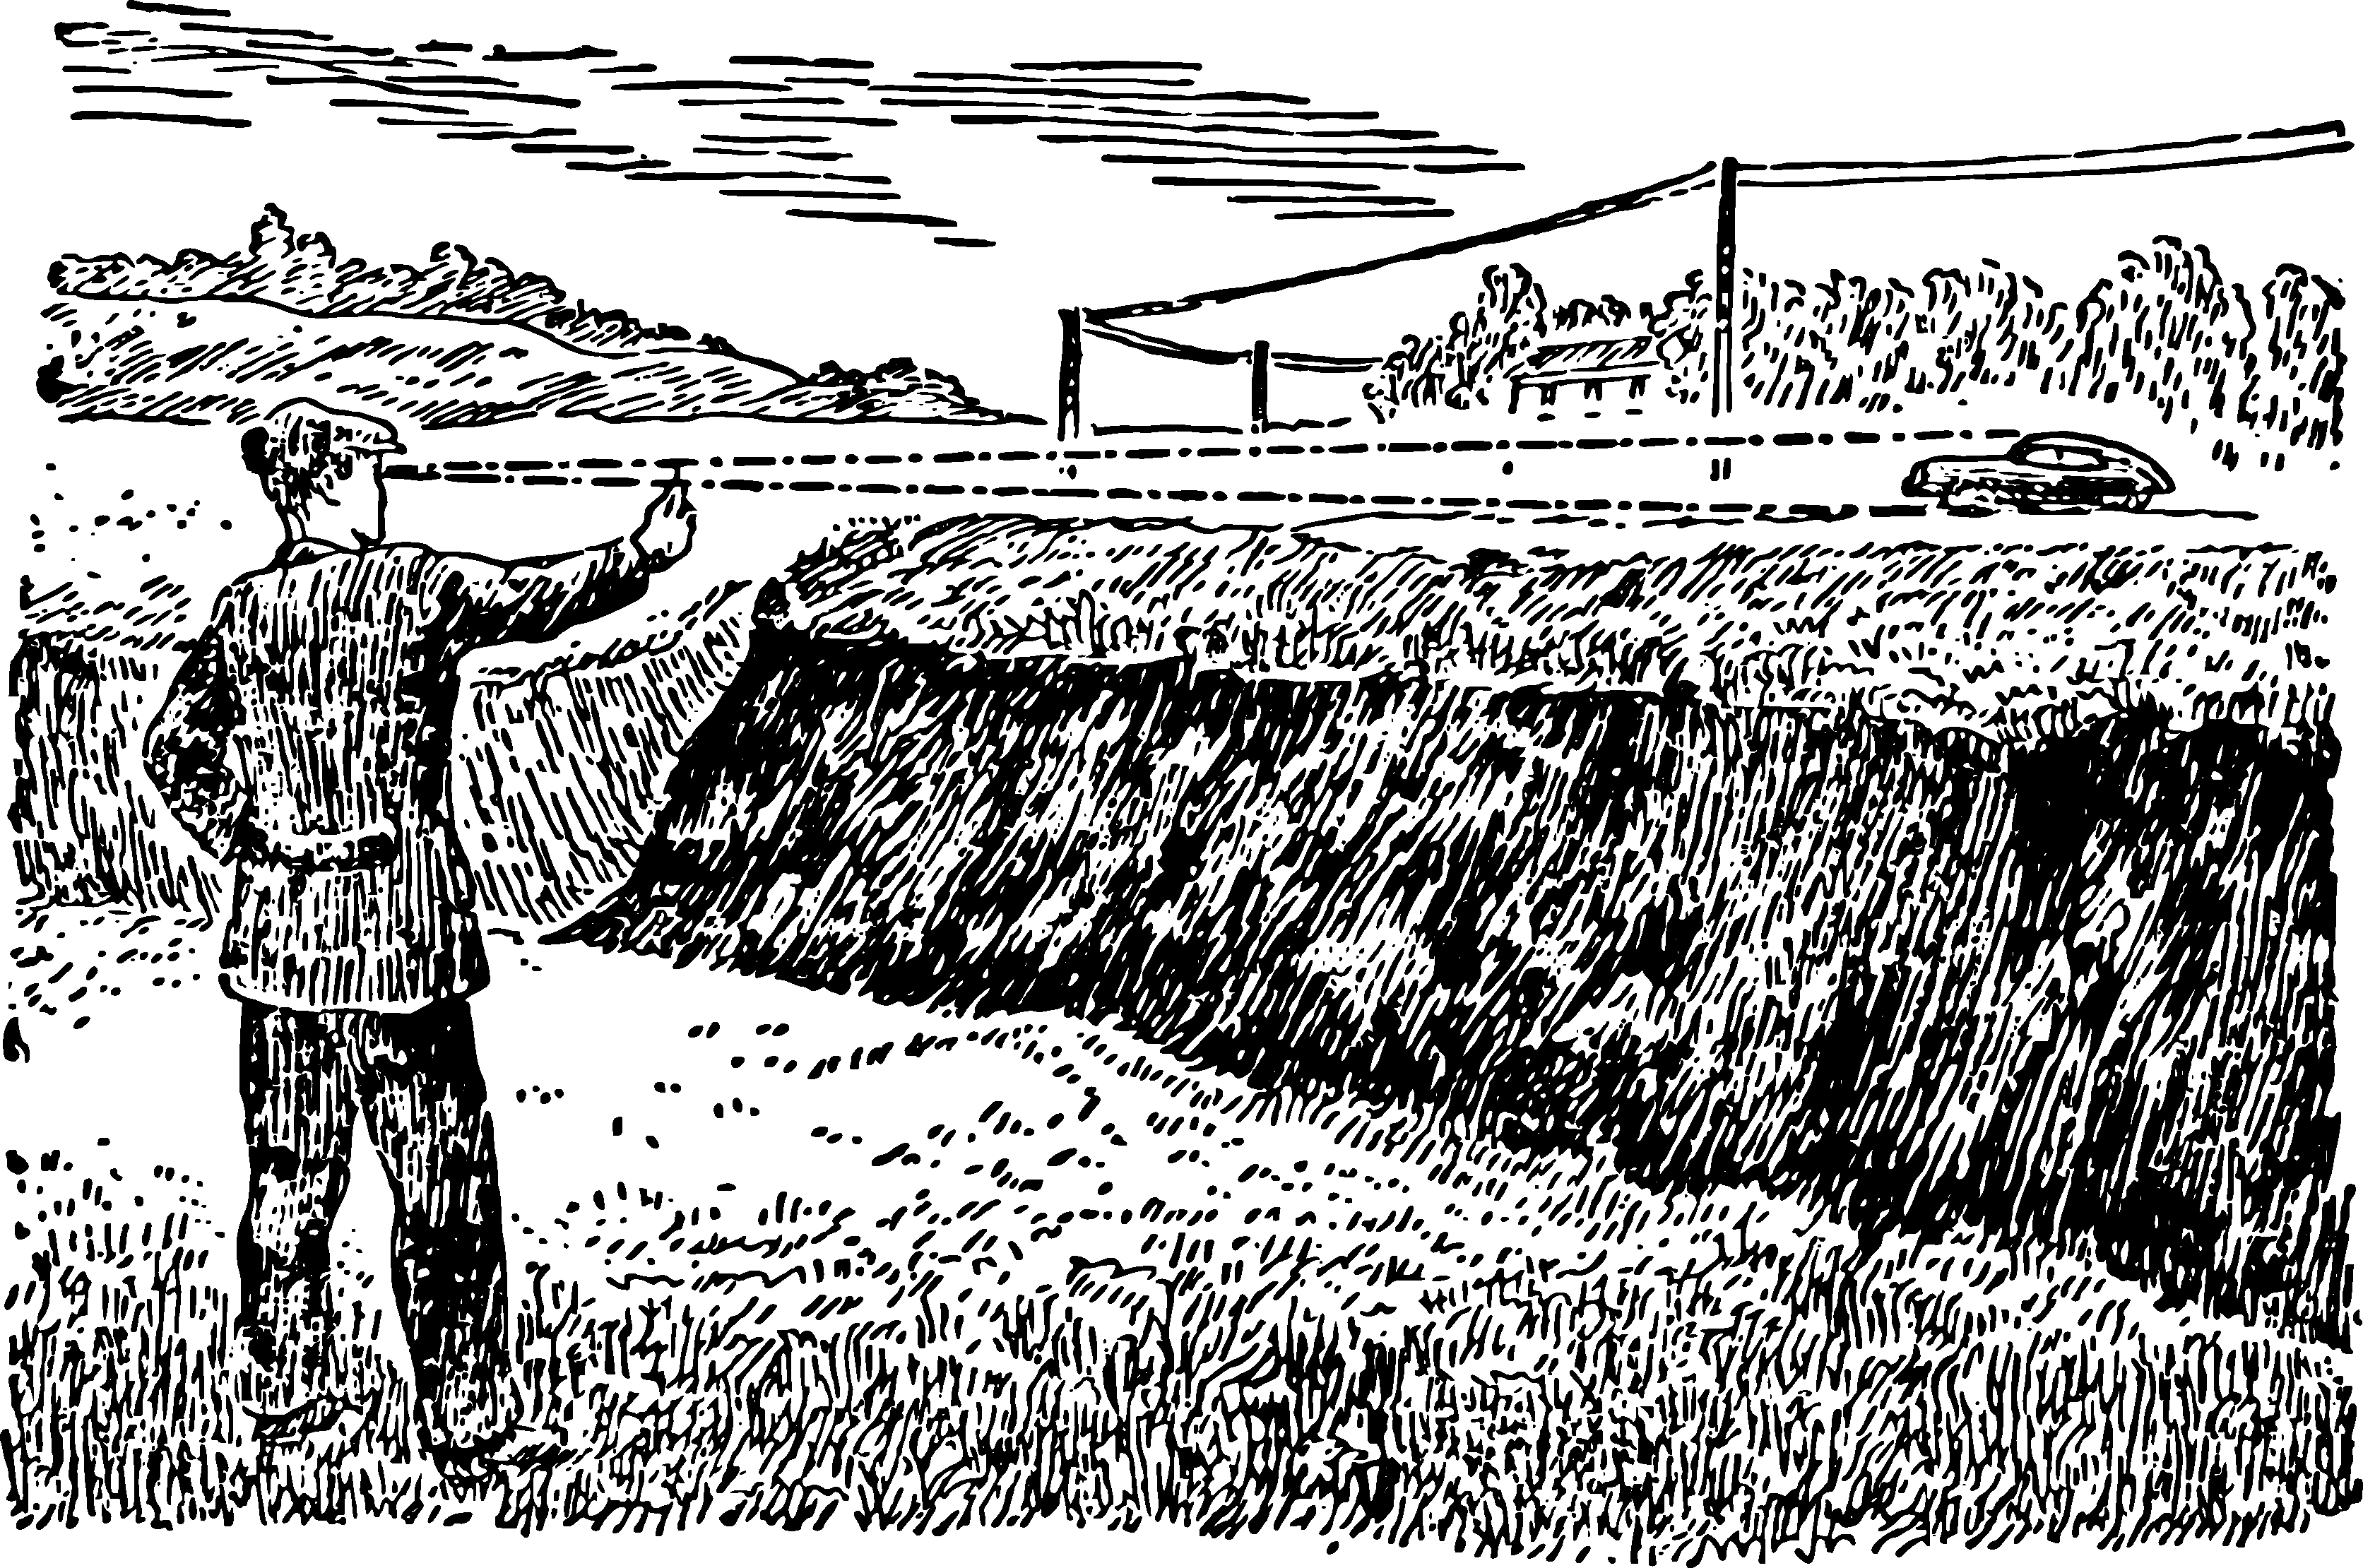
\includegraphics[width=\textwidth]{figures/ch-02/fig-038.pdf}
\sidecaption[][-5cm]{The use of a rangefinder match to determine inaccessible distances.\label{fig-038}}
\end{figure}

You can easily verify the correctness of the proportion:
\begin{equation*}%
\frac{\text{desired distance}}{\begin{array}{c}\text{distance from the eye}\\ \text{to the matchstick}\end{array}} = \frac{\text{average height of a person}}{\begin{array}{c}\text{measured part}\\ \text{of the matchstick}\end{array}}
\end{equation*}
From here, it's easy to calculate the desired distance. For example, if the distance to the matchstick is \SI{60}{\centi\meter}, the height of the person is \SI{1.7}{\meter}, and the measured part of the matchstick is \SI{12}{\milli\meter}, then the determined distance would be:
\begin{equation*}%
60 \cdot \frac{1700}{12} = \SI{8500}{\centi\meter} = \SI{85}{\meter}.
\end{equation*}
To gain some skill in using this rangefinder, measure the height of someone from your group and, asking them to move away a certain distance, try to determine how many steps they took away from you.

\begin{marginfigure}[-3cm]%[h!]
\centering
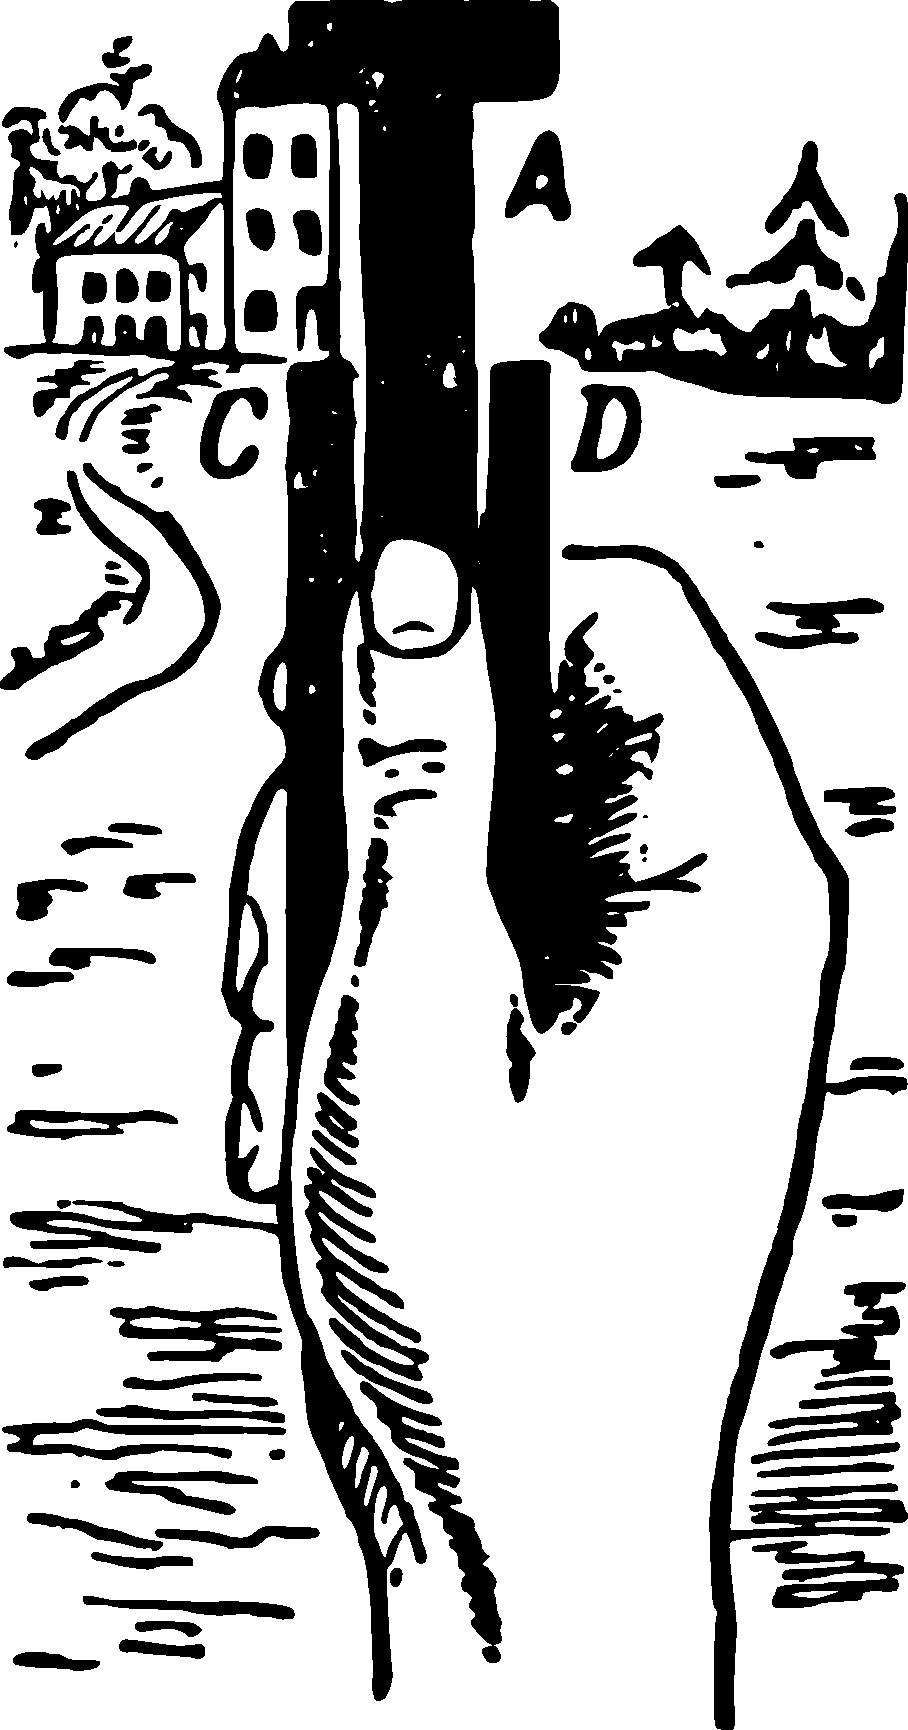
\includegraphics[width=0.8\textwidth]{figures/ch-02/fig-039.pdf}
\sidecaption{The retractable rangefinder in action.\label{fig-039}}
\end{marginfigure}

With the same method, you can determine the distance to a rider (average height \SI{2.2}{\meter}), a cyclist (wheel diameter \SI{75}{\centi\meter}), a telegraph pole along the railway track (height \SI{8}{\meter}), vertical distance between adjacent insulators (\SI{90}{\centi\meter}), to a train, a brick house, and similar objects whose dimensions can be estimated with sufficient accuracy. There can be quite a few such cases during excursions.



For those skilled in crafting, making a more convenient device of the same type, intended for estimating distances based on the size of a distant human figure, won't be much trouble.

\begin{marginfigure}[-2cm]%[h!]
\centering
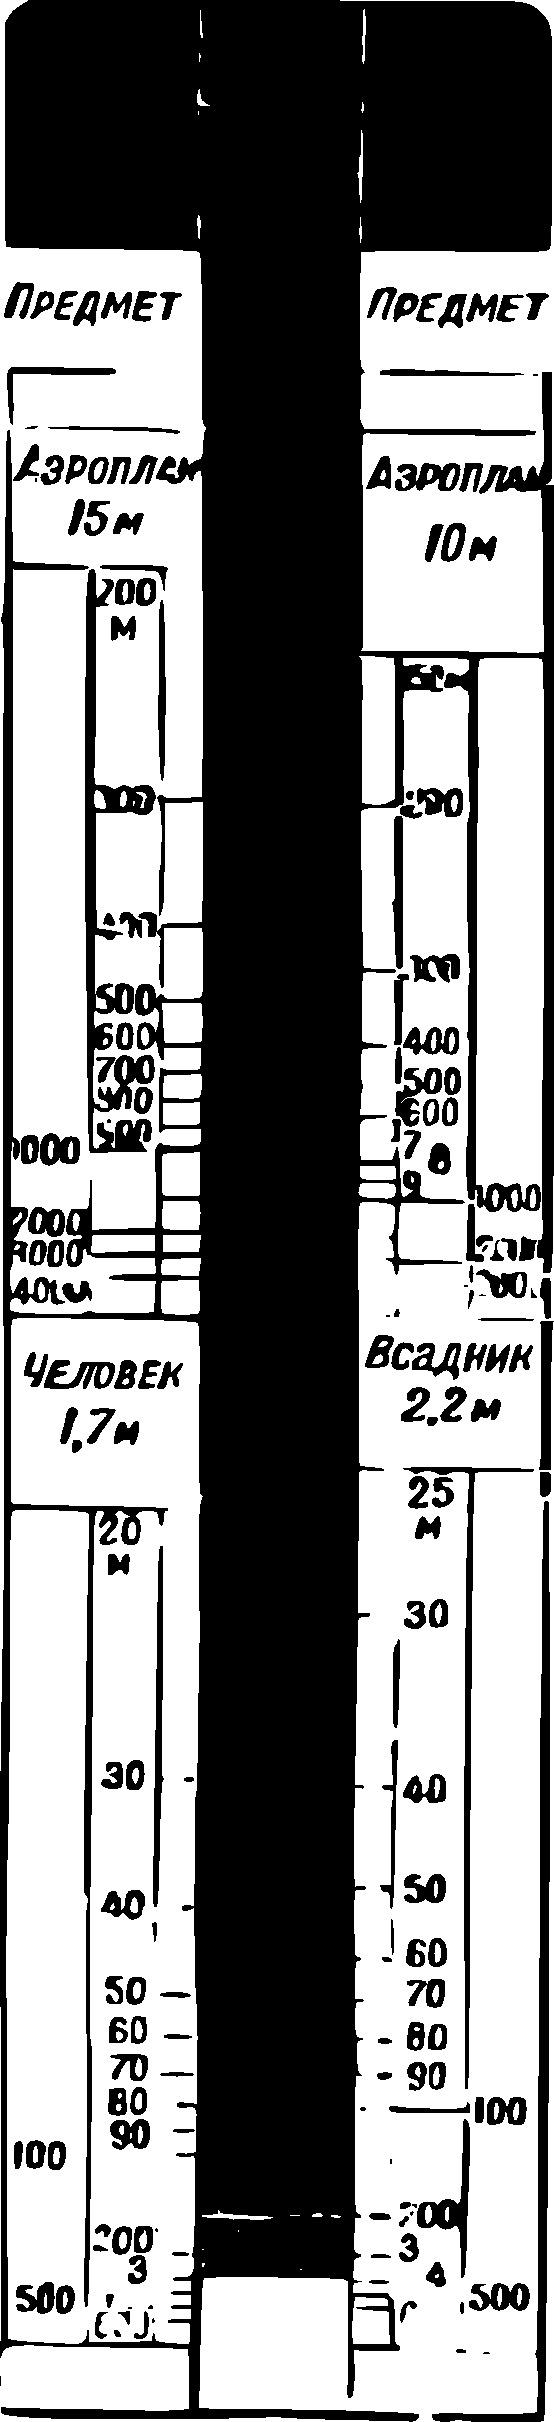
\includegraphics[width=0.6\textwidth]{figures/ch-02/fig-040.pdf}
\sidecaption{The design of the retractable rangefinder.\label{fig-040}}
\end{marginfigure}

The device is clear in \figr{fig-039} and \figr{fig-040}. The observed object is placed precisely in the gap $A$, formed when the extension part of the device is raised. The size of the gap can be conveniently determined by the divisions on the part $C$ and $D$ of the board. To avoid the need for any calculations, you can directly mark on strip $C$ the distances corresponding to the divisions if the observed object is a human figure (the device for measuring the distance of the outstretched arm). On the right strip $D$, you can mark distances, pre-calculated for cases where a rider is observed (\SI{2.2}{\meter}). For telegraph poles (height \SI{8}{\meter}), planes with a wingspan of \SI{15}{\meter}, and other larger objects, you can use the upper, free parts of strips $C$ and $D.$ Then the device will look like the one presented in \figr{fig-040}.





Of course, the accuracy of such distance estimation is low. It's just an estimate, not a measurement. In the example discussed earlier, where the distance to the human figure was estimated at \SI{85}{\meter}, an error of \SI{1}{\milli\meter} in measuring the matchstick portion would result in a deviation of \SI{7}{\meter} (1/12 out of 85). But if the person stood four times farther away, and we measured only \SI{3}{\milli\meter} on the matchstick, then an error of even 1/2 mm would cause a change in the result by \SI{57}{\meter}. Therefore, our example is reliable only for relatively short distances -- in the range of 100--200 m. When estimating larger distances, it's necessary to choose larger objects.


\section{The energy of the river}
\label{sec-2.6}

\begin{quote}
\emph{You know the edge where everything breathes abundance,\\
Where rivers flow purer than silver, \\
Where the steppe breeze sways the feather grass, \\
Where villages are nestled in cherry orchards.}\\[-10pt]
\flushright{\emph{A.K. Tolstoy}}
\end{quote}


A river, the length of which is no more than 100 km, is considered small. Do you know how many such small rivers there are in the USSR? A lot -- 48 thousand!

If these rivers were stretched into a single line, it would result in a ribbon \SI{13800000}{\kilo\meter} long. With such a ribbon, you could encircle the Earth at the equator thirty times (the length of the equator is approximately \SI{40009}{\kilo\meter}).

The flow of these rivers is leisurely, but it conceals an inexhaustible supply of energy within it. Specialists believe that if the hidden potential of all the small rivers flowing through our homeland were combined, an impressive number would be obtained -- 34 million kilowatts! This gifted energy needs to be widely utilised for electrifying the economy of settlements located near rivers.

\begin{quote}
\emph{Let the river flow freely,\\
If the plan says so,\\
A dam with a stone ridge across all depths\\
Will block the way forever.}\\[-10pt]
\flushright{\emph{S. Shchipachev}}
\end{quote}

You know that this is achieved through hydroelectric power stations (HPS), and you can show a lot of initiative and provide real assistance in preparing for the construction of small HPS. Indeed, the builders of HPS will be interested in everything related to the river regime: its width and flow rate (``water flow''), the area of the cross-section of the riverbed (``active section''), and what water head the banks allow. And all this can be measured with available means and represents a relatively simple geometric problem.

We will now proceed to solving this problem.

But first, let's present here a practical advice from specialists, engineers V. Yarosh and I. Fedorov, regarding the selection of a suitable location on the river for the construction of a future dam.

They recommend building a small hydroelectric power station with a capacity of 15-20 kilowatts ``no further than 5 km from the village.''

``The dam of an HPS should be built no closer than 10-15 km and not farther than 20-40 km from the source of the river because moving away from the source entails the costly reinforcement of the dam, which is caused by a large influx of water. If the dam is located closer than 10-15 km from the source, due to the small water flow and insufficient head, the hydroelectric power station will not be able to provide the necessary power. The chosen stretch of the river should not be abundant in great depths, which also increases the cost of construction, requiring a heavy foundation.''

\section{The Flow Rate}
\label{sec-2.7}
\begin{quote}
\emph{Between village and mountain grove,\\
Winds a river like a bright ribbon.}\\[-10pt]
\flushright{\emph{A. Fet}}
\end{quote}

How much water flows in such a river in a day? It's easy to calculate if you first measure the speed of the water flow in the river. The measurement is performed by two people. One person holds a watch, the other holds some noticeable float, for example, a half-empty bottle with a flag. They choose a straight section of the river and place two stakes $A$ and $B$ along the bank at a distance, for example, \SI{10}{\meter} from each other (see \figr{fig-041}).

\begin{figure}[h!]
\centering
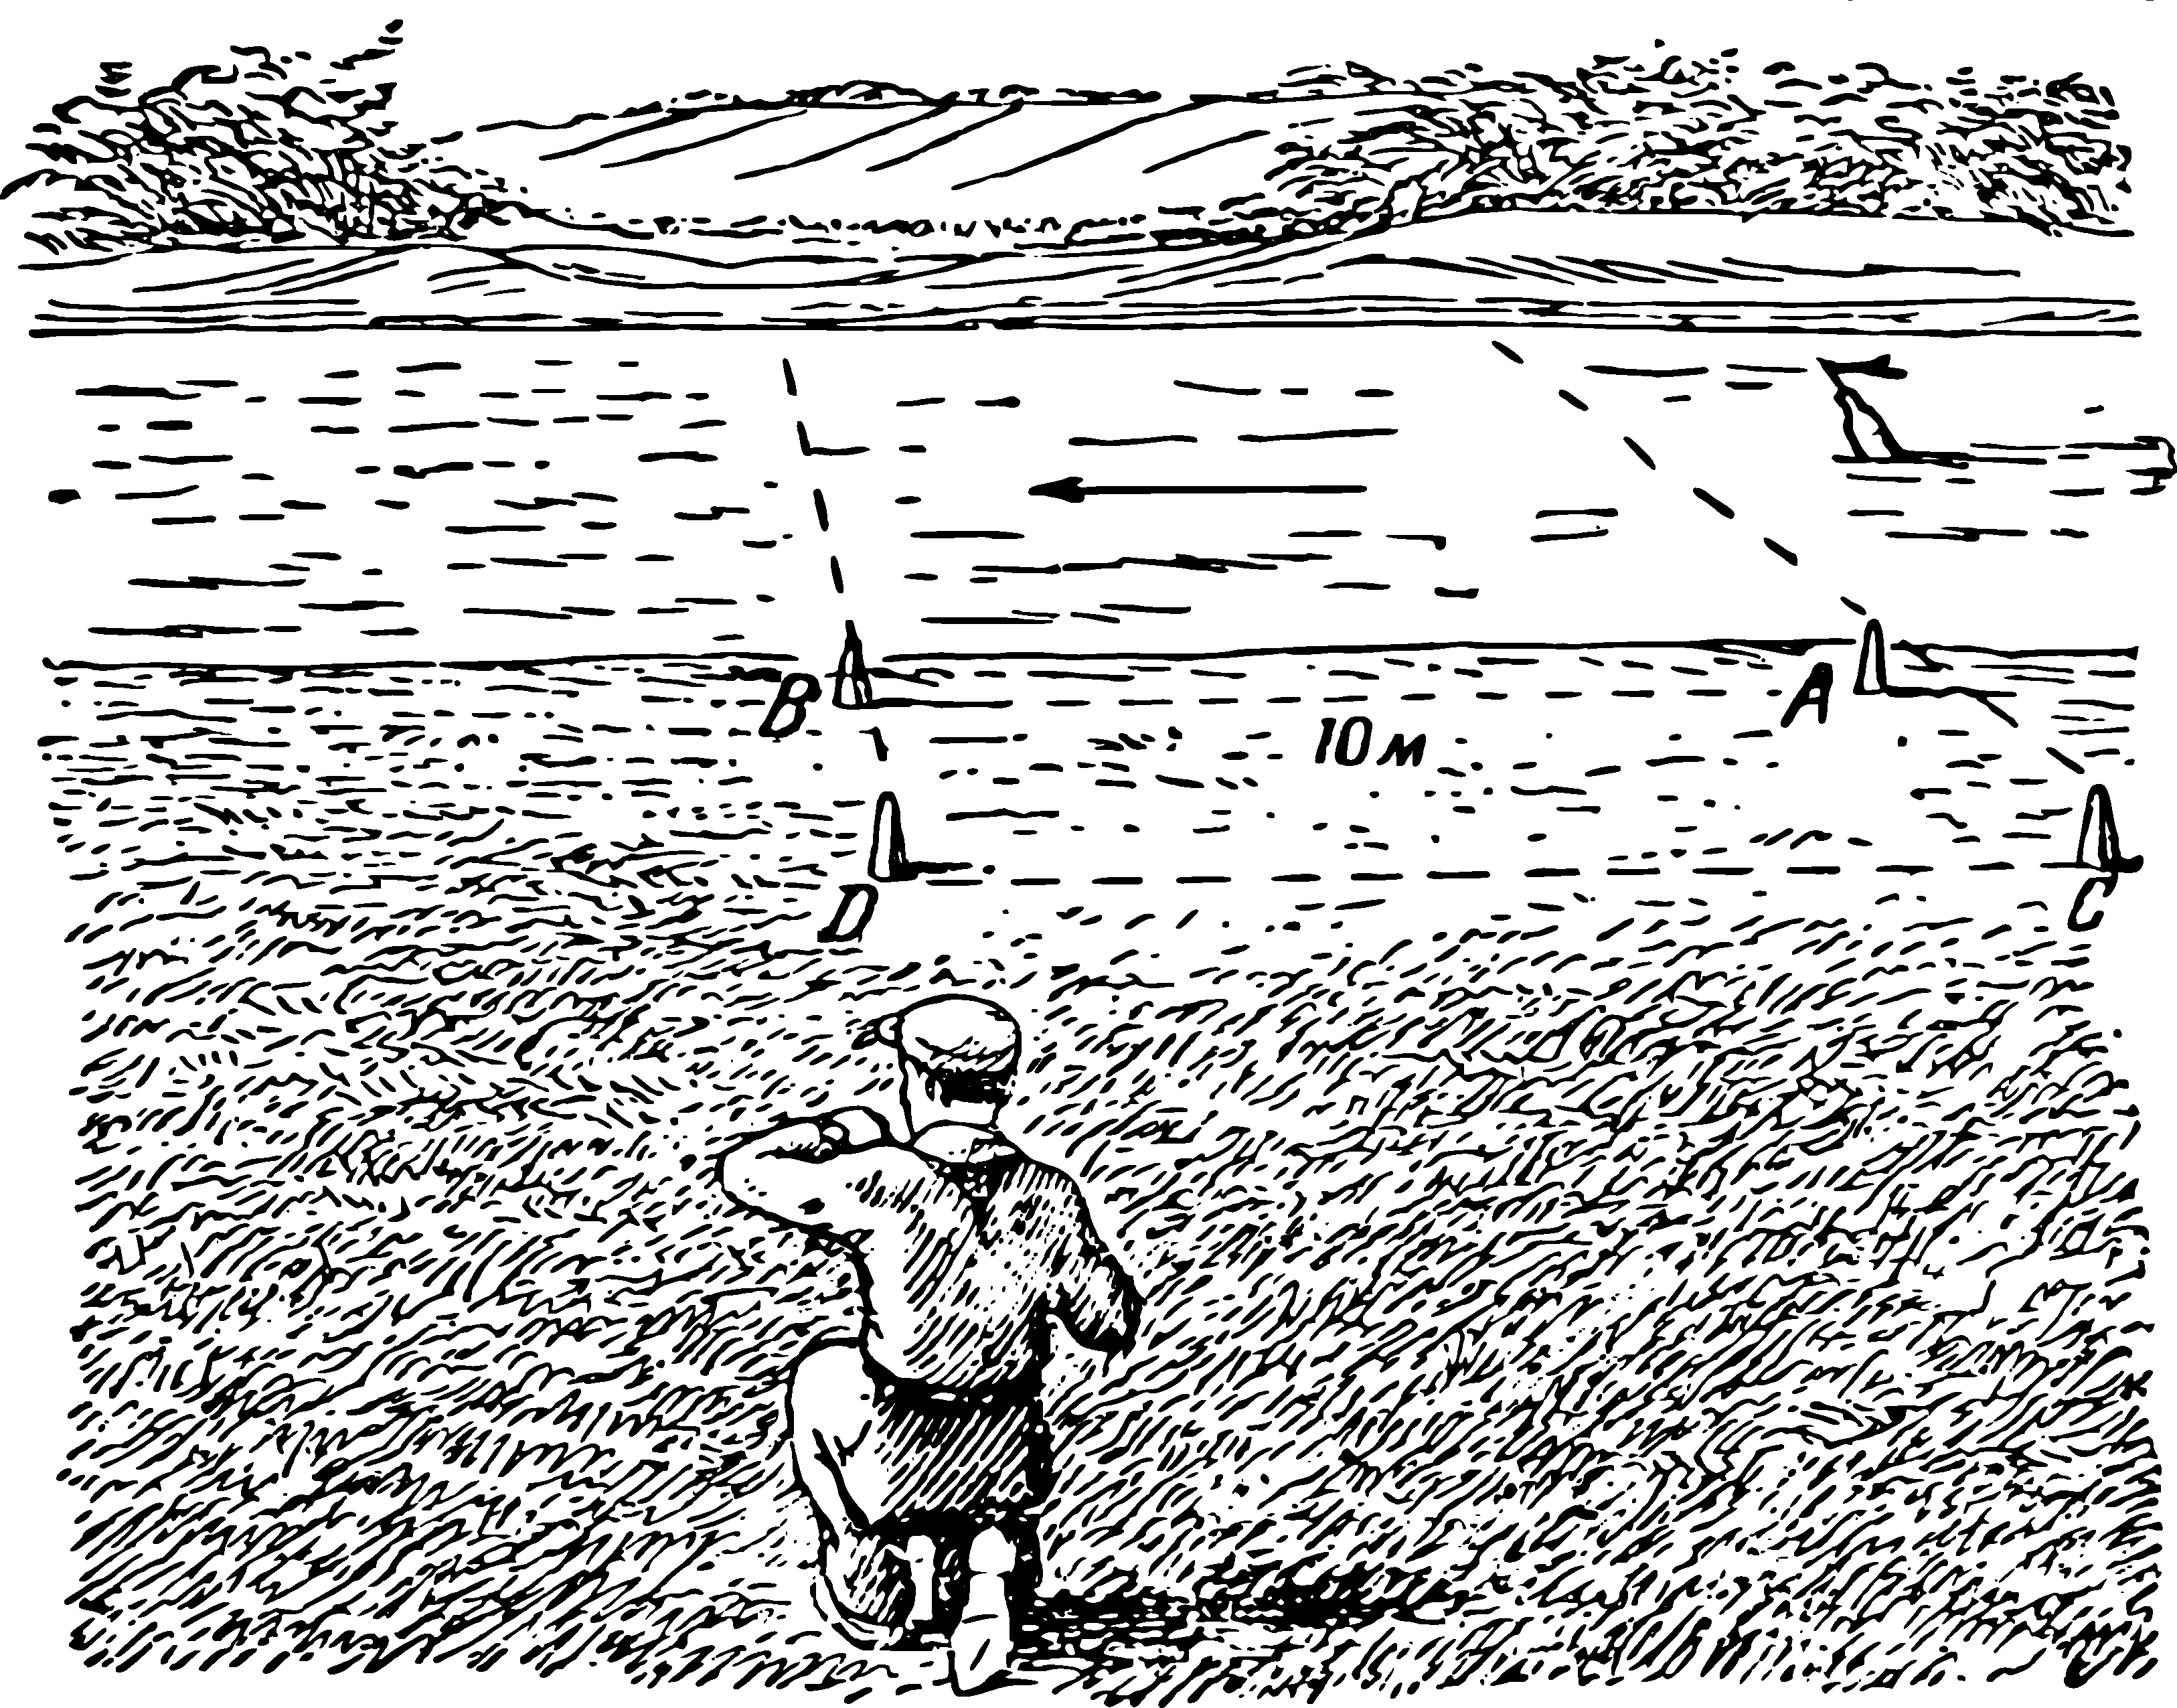
\includegraphics[width=0.9\textwidth]{figures/ch-02/fig-041.pdf}
\sidecaption{Measurement of the river flow velocity.\label{fig-041}}
\end{figure}

Two more stakes $C$ and $D$ are placed on lines perpendicular to $AB$. One of the participants in the measurement with the watch stands behind stake $D$. The other, with the float, goes a bit upstream of stake $A$, throws the float into the water, and then stands behind stake $C$. Both observers look along the directions $CA$ and $DB$ towards the water surface. At the moment when the float crosses the extension of the line $CA$, the first observer waves his hand. Upon this signal, the second observer starts the timer for the first time and then again when the float crosses the direction of $DB$.

Let's assume that the time difference is 20 seconds.

Then the speed of the water flow in the river is:
\begin{equation*}%
\frac{10}{20} = \SI{0.5}{\meter\per\second}.
\end{equation*}
Usually, the measurement is repeated about ten times\sidenote{Instead of throwing one float ten times, you can immediately throw 10 floats at some distance from each other.}, throwing the float into different points on the river surface. Then the obtained numbers are summed up and divided by the number of measurements. This gives the average speed of the surface layer of the river.

Deeper layers flow slower, and the average speed of the entire flow is approximately 4/5 times the surface speed. In our case, therefore, it's \SI{0.4}{\meter\per\second}.

You can determine the surface speed by another -- albeit less reliable -- method.

Sit in a boat and paddle \SI{1}{\kilo\meter} (measured along the shore) against the current, and then back -- with the current, trying to paddle with the same force all the time.

Let's say you paddled these \SI{1000}{\meter} against the current in 18 minutes, and with the current in 6 minutes. Denoting the desired speed of the river current as $x$, and the speed of your movement in still water as $y$, you form the equations:
\begin{equation*}%
\frac{1000}{y - x} = 18, \qand \frac{1000}{y + x} = 6.
\end{equation*}
Rearranging we get:
\begin{equation*}%
y + x = \frac{1000}{6}, \qand y - x = \frac{1000}{18}.
\end{equation*}
Solving for $x$, we get $2x = 110$, and $x = 55$. The speed of the water flow on the surface is 55 m per minute, and therefore, the average speed is about 5/6 \si{\meter\per\second}.


\section{How Much Water Flows In The River?}
\label{sec-2.08}

To measure the amount of water flowing in a river, you can always determine the speed at which the water flows. The more challenging part of the preparatory work needed to calculate the quantity of flowing water is to determine the cross-sectional area of the water. To find the magnitude of this area, known as the ``live cross-section'' of the river, you need to make a drawing of this section. Such work is done as follows.

\textbf{First Method:} At the point where you measured the width of the river, you drive a stake into the ground on both banks, right at the water's edge. Then, with a companion, you get into a boat and row from one stake to the other, trying to keep a straight line connecting the stakes. An inexperienced rower will not be able to handle such a task, especially in a river with a fast current. Your companion must be a skilled rower; besides, a third participant in the work should stand on the bank, ensuring that the boat stays on the correct course and giving the rower signals indicating which way to turn when necessary. During the first crossing of the river, you only need to count how many strokes of the oars it took and from there figure out how many strokes move the boat 5 or 10 meters. Then, for the second crossing, armed with a sufficiently long rake with markings on it, you plunge the rake vertically to the bottom every 5-10 meters (measured by the number of oar strokes) and record the depth of the river at that point.

This method can only measure the live cross-section of a small river; for a wide, multi-water river, more complex methods are needed, which are performed by specialists. An amateur must choose a task that suits their modest measuring means.

\textbf{Second Method:} On a narrow and shallow river, you don't need a boat.

Between the stakes, you stretch a cord perpendicular to the current with marks or knots made on it every 1 or 2 meters, and by lowering a ruler to the bottom at each knot, you measure the depth of the riverbed. When all measurements are done, you first draw a millimeter paper or a grid paper sketch of the cross-section profile of the river. You will get a figure similar to the one shown in \figr{fig-042}. It is quite easy to determine the area of this figure since it can be divided into a series of trapezoids (where both bases and the height are known) and two side triangles, also with known base and height. If the scale of the drawing is 1:100, then the result will be obtained directly in square meters.

\begin{figure}[h!]
\centering
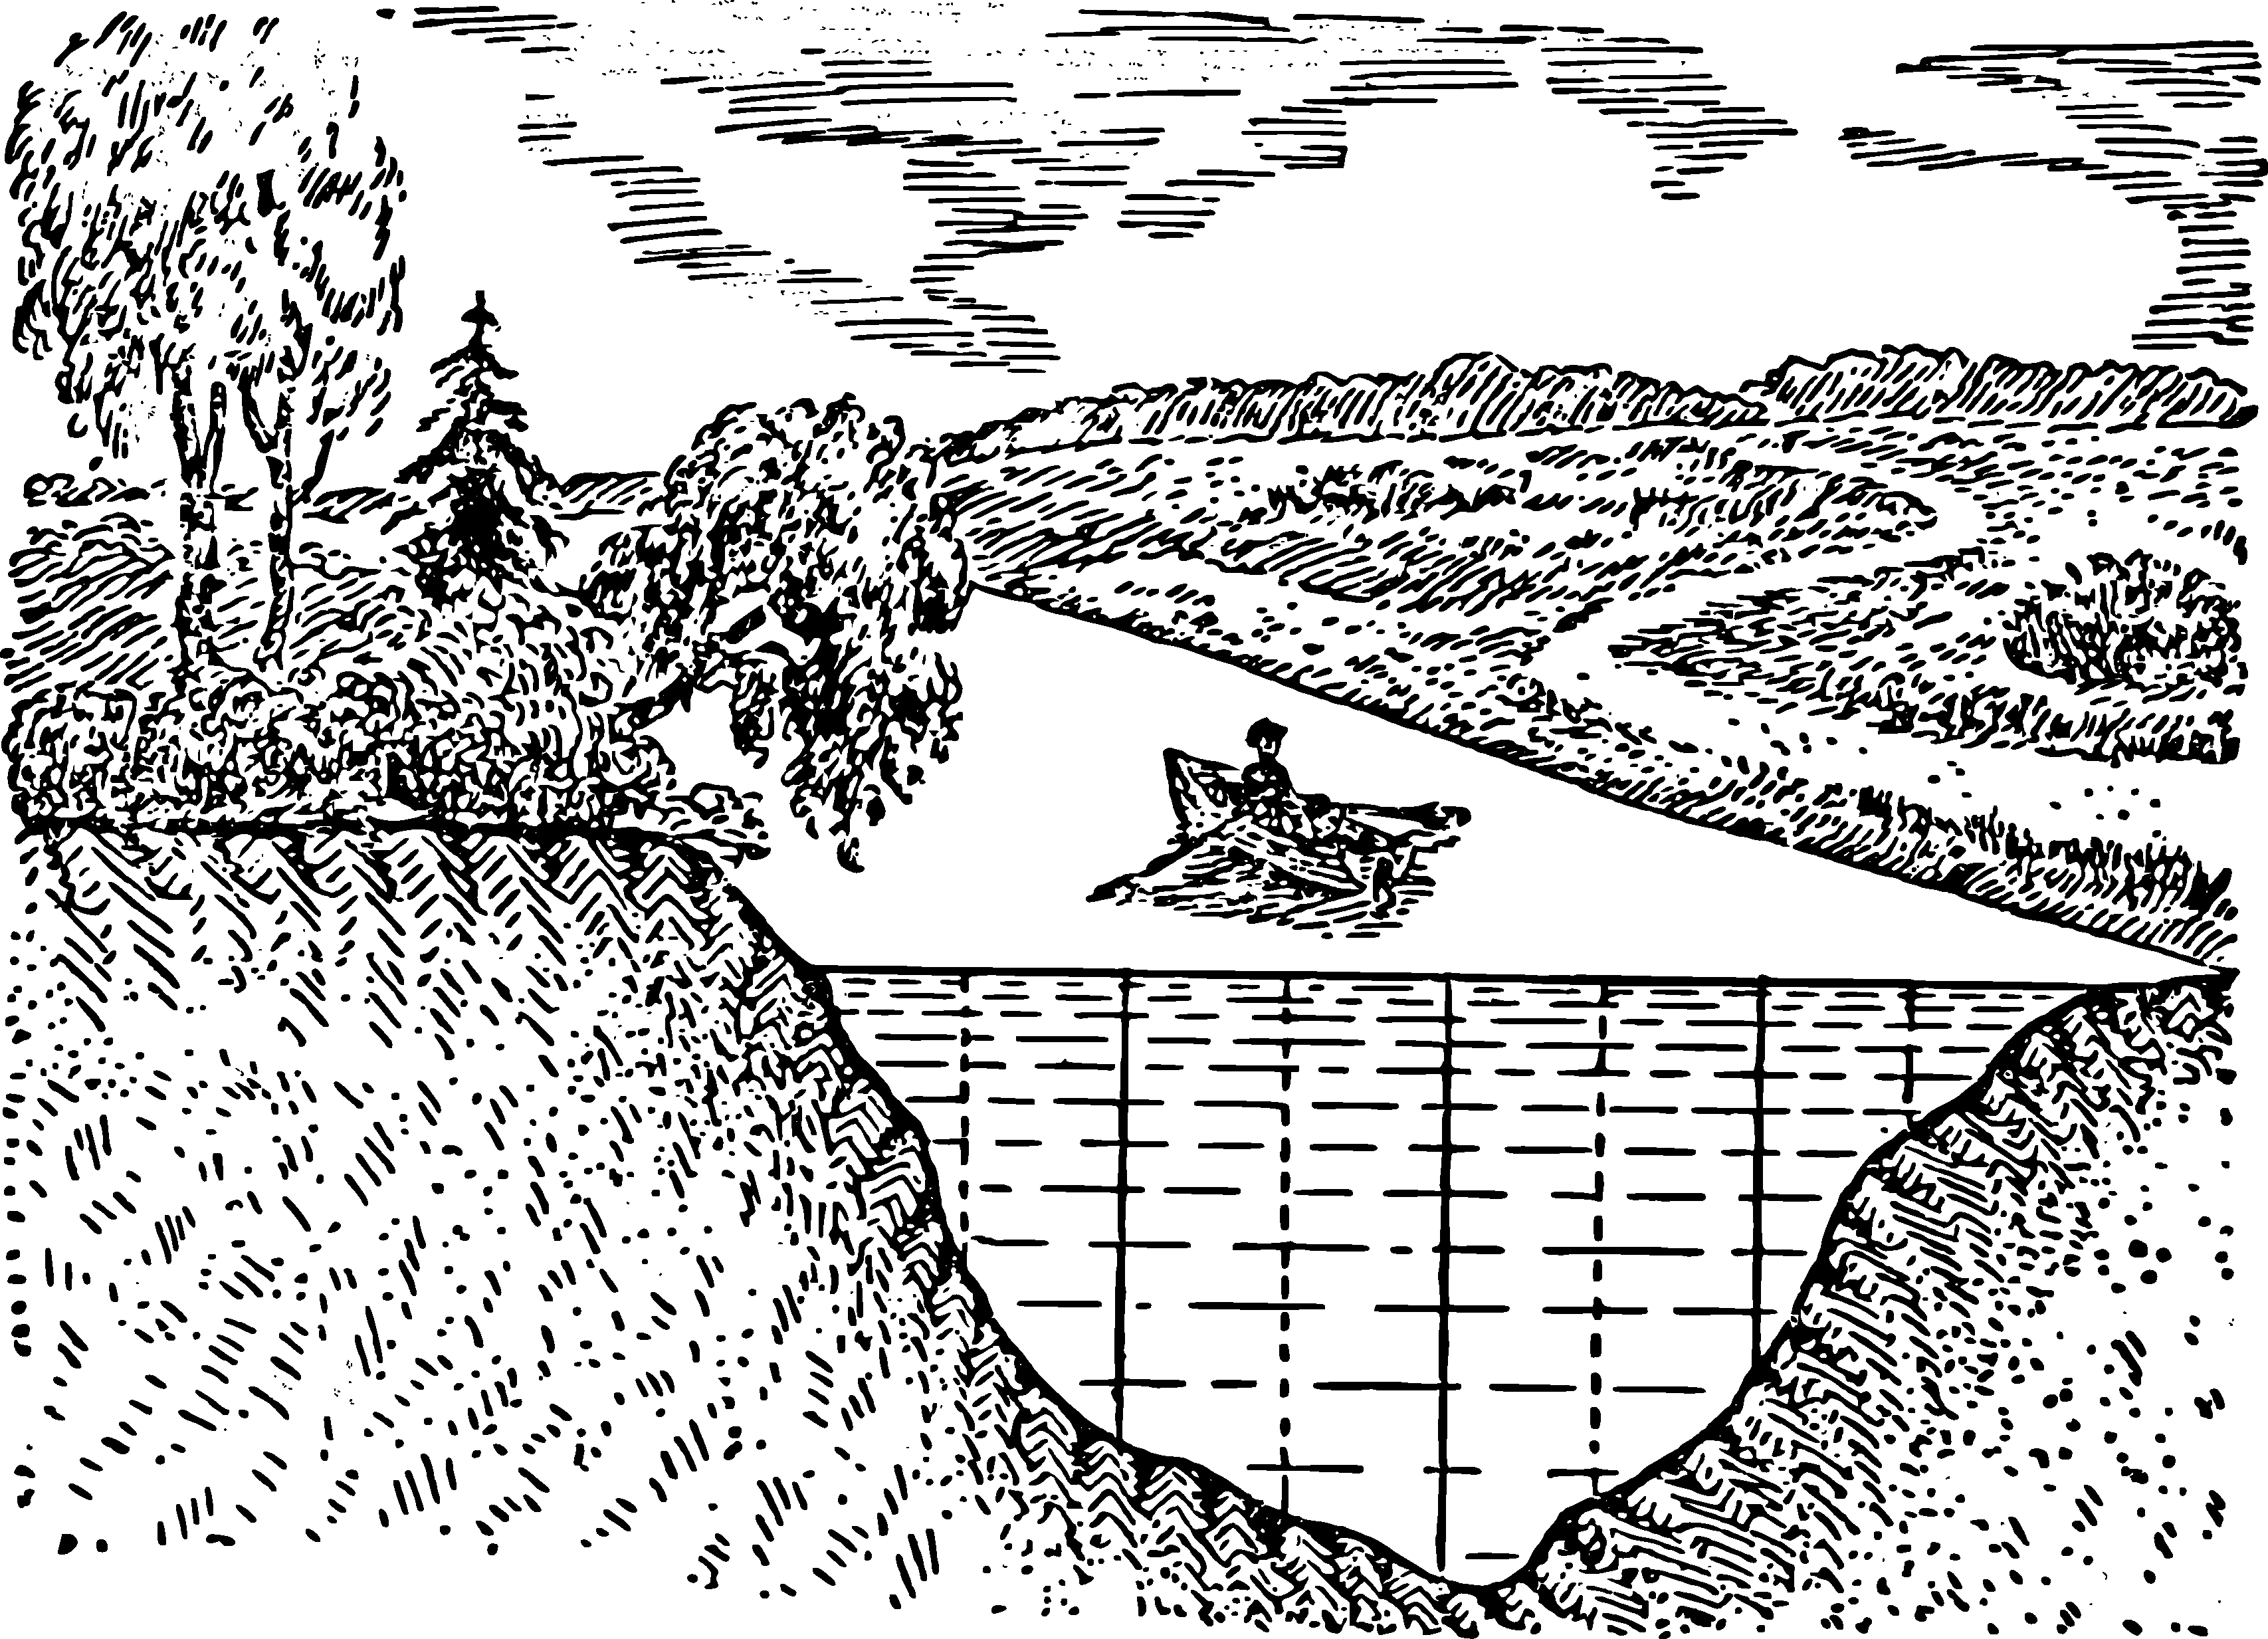
\includegraphics[width=0.9\textwidth]{figures/ch-02/fig-042.pdf}
\sidecaption{``Live Cross-Section'' of a River.\label{fig-042}}
\end{figure}

Now you have all the data needed to calculate the amount of flowing water. Obviously, through the live cross-section of the river, a volume of water equal to the volume of a prism is passing every second, where the cross-section serves as the base and the average second-by-second flow rate serves as the height. For example, if the average flow rate of water in the river is 0.4 meters per second, and the area of the live cross-section is, let's say, 3.5 square meters, then every second, through this section, there will be a transfer of
\begin{equation*}%
3.5 \times 0.4 = 1.4 \,\, \text{cubic meters of water},
\end{equation*}
or the same amount in tons\sidenote{1 cubic meter of fresh water weighs 1000 kg.} This amounts to 
\begin{align*}%
1.4 \times 3600 & = 5040 \,\, \text{cubic meters of water per hour, and}\\
5040 \times 24 & = \num{120960} \,\, \text{cubic meters of water per day},
\end{align*}
which is over a hundred thousand cubic meters. And yet, a river with a live cross-section of 3.5 square meters is a small river; it could be, for example, 3.5 meters wide and 1 meter deep at a fordable point. But even it contains energy capable of transforming into mighty electricity. So how much water flows per day in a river like the Neva, through which 3300 cubic meters of water pass every second through its live cross-section! This is the ``average flow rate'' of water in the Neva at Leningrad. The ``average flow rate'' of water in the Dnieper at Kiev is 700 cubic meters.

\begin{figure}[h!]
\centering
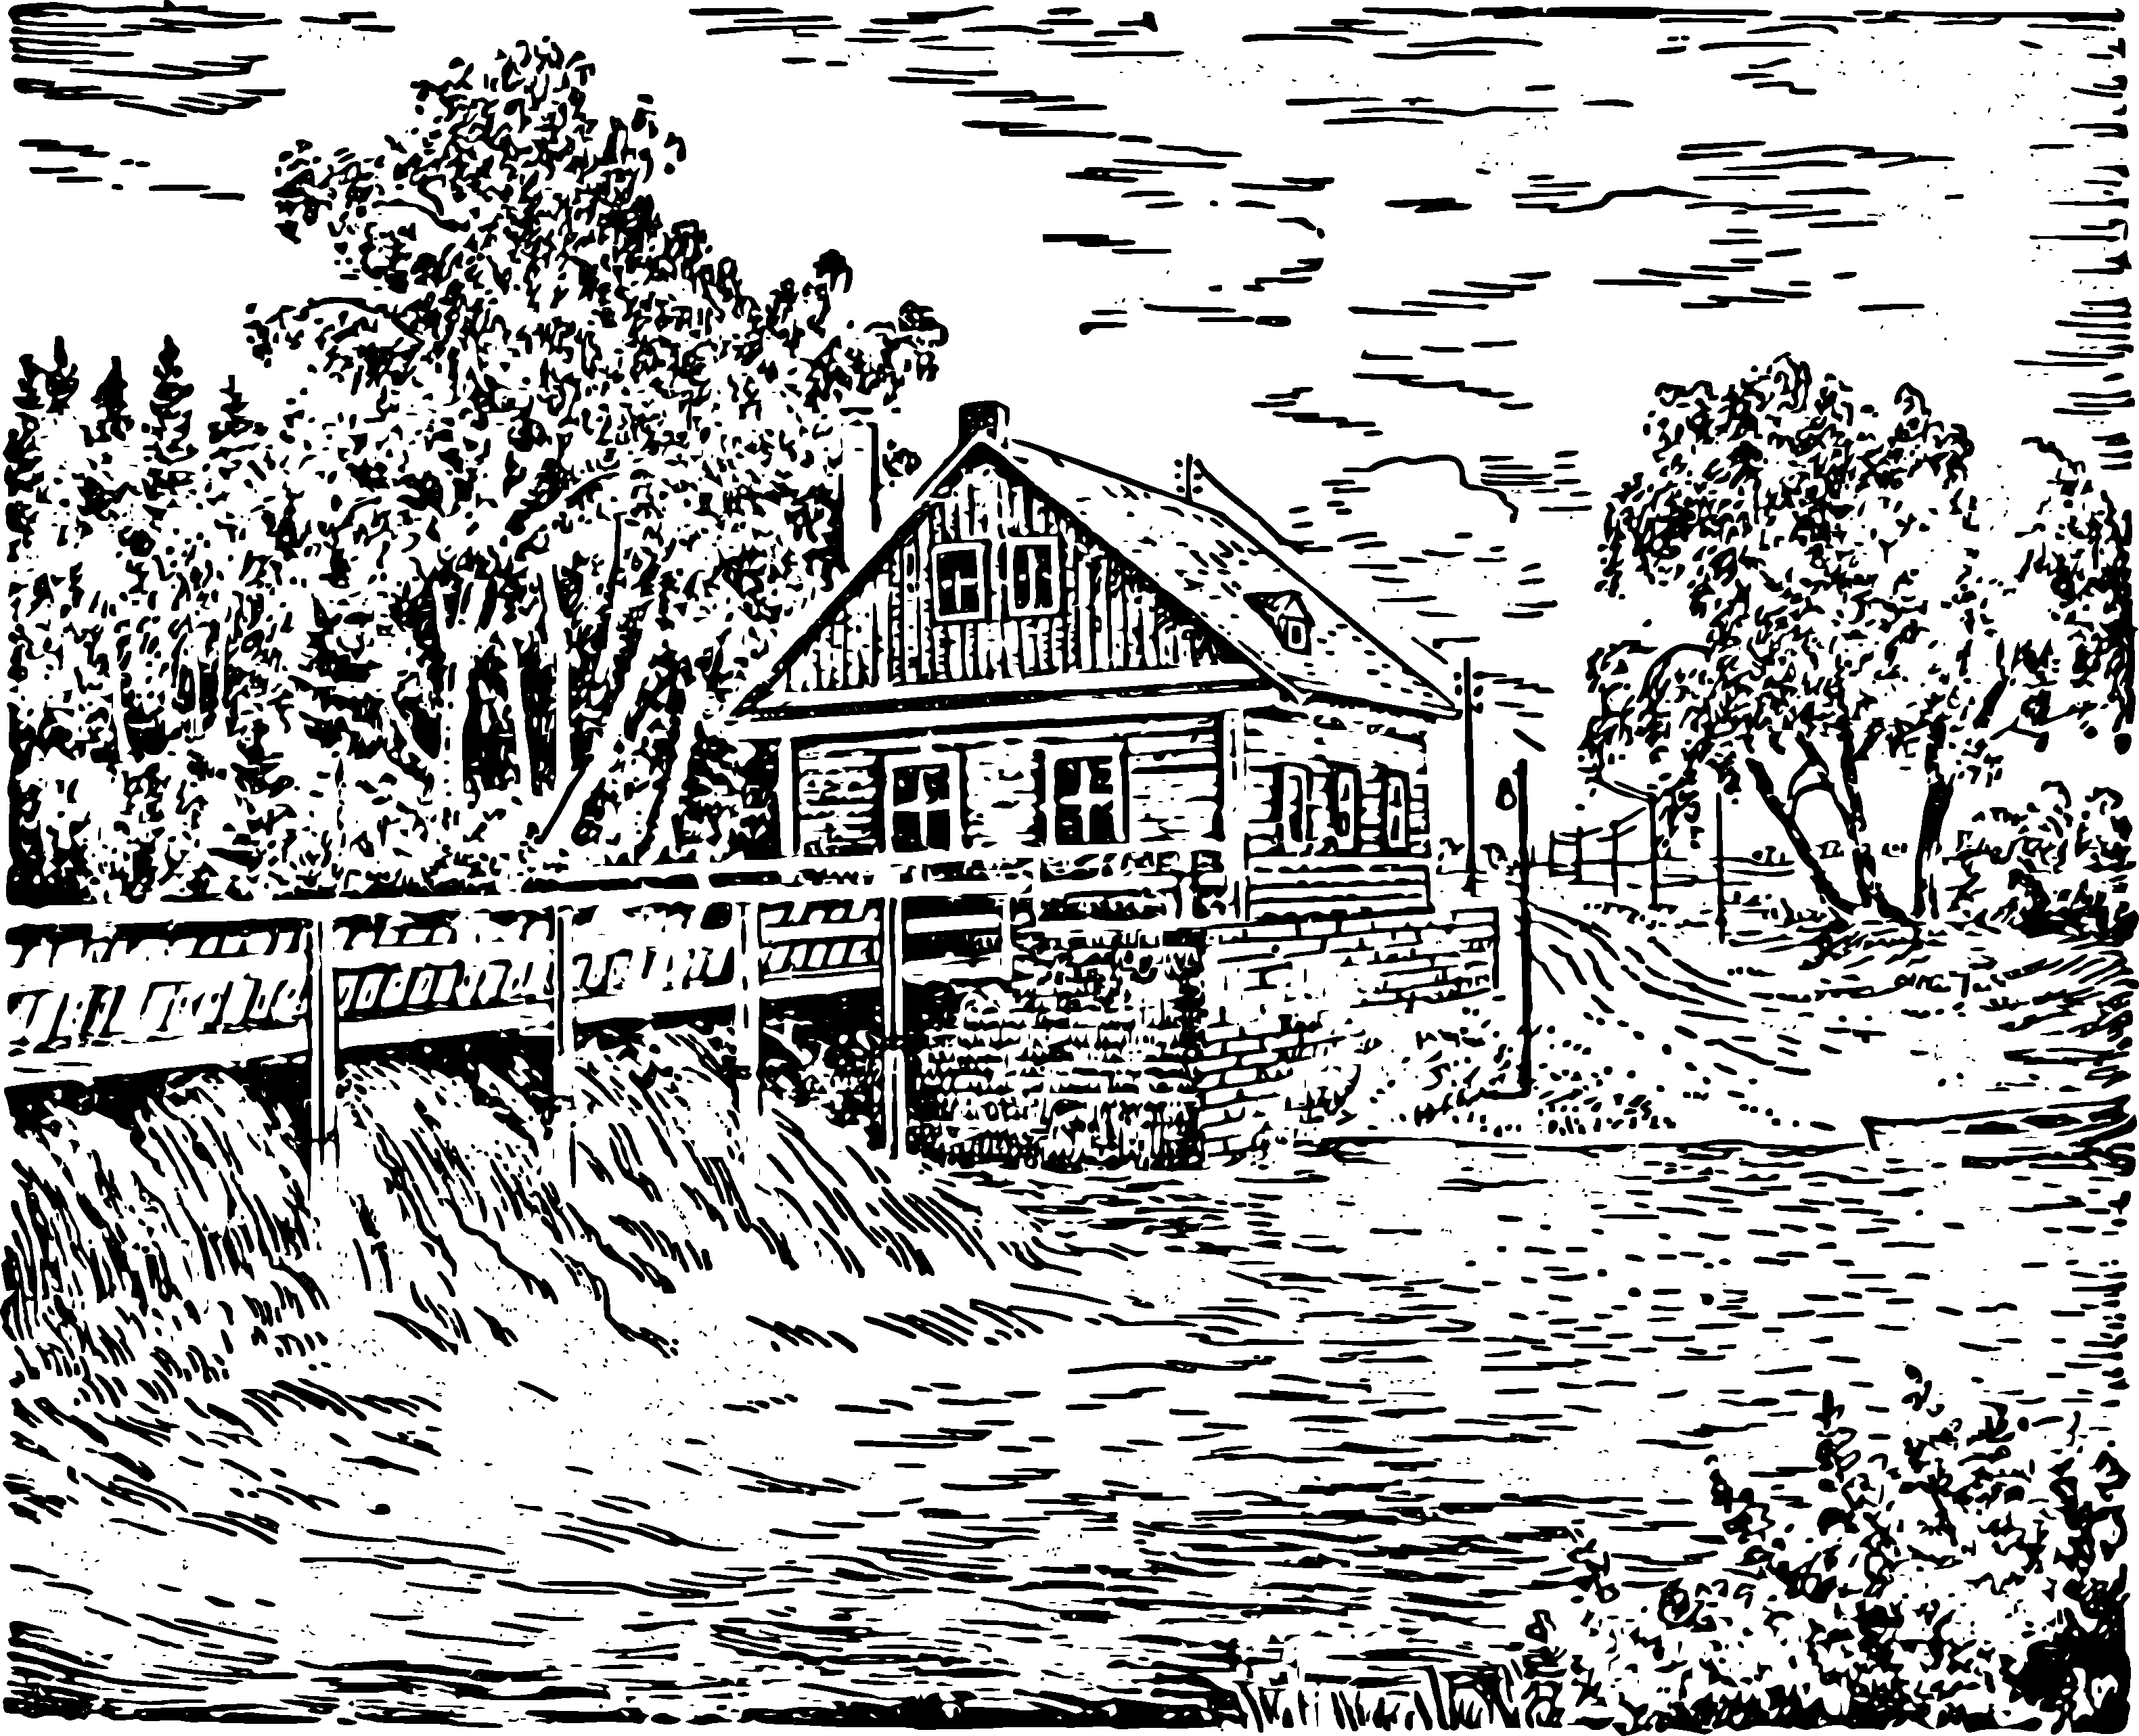
\includegraphics[width=\textwidth]{figures/ch-02/fig-043.pdf}
\sidecaption{The hydroelectric power station with a capacity of 80 kilowatts belongs to the Burmakin Agricultural Collective Farm and provides energy to seven collective farms.\label{fig-043}}
\end{figure}

Young explorers and future dam builders also need to determine the maximum head the banks can allow, i.e., the difference in water levels that the dam can create (\figr{fig-043}). To do this, stakes are driven into the banks 5-10 meters away from the water, as usual, along a line perpendicular to the river's current. Then, moving along this line, small stakes are placed at points of characteristic bends in the banks (\figr{fig-044}). Using rulers with markings, the elevation of one stake above the other and the distances between them are measured. Based on the measurement results, a profile of the banks is drawn similar to the profile of the riverbed. The bank profile can indicate the magnitude of the allowable head.

\begin{figure}[h!]
\centering
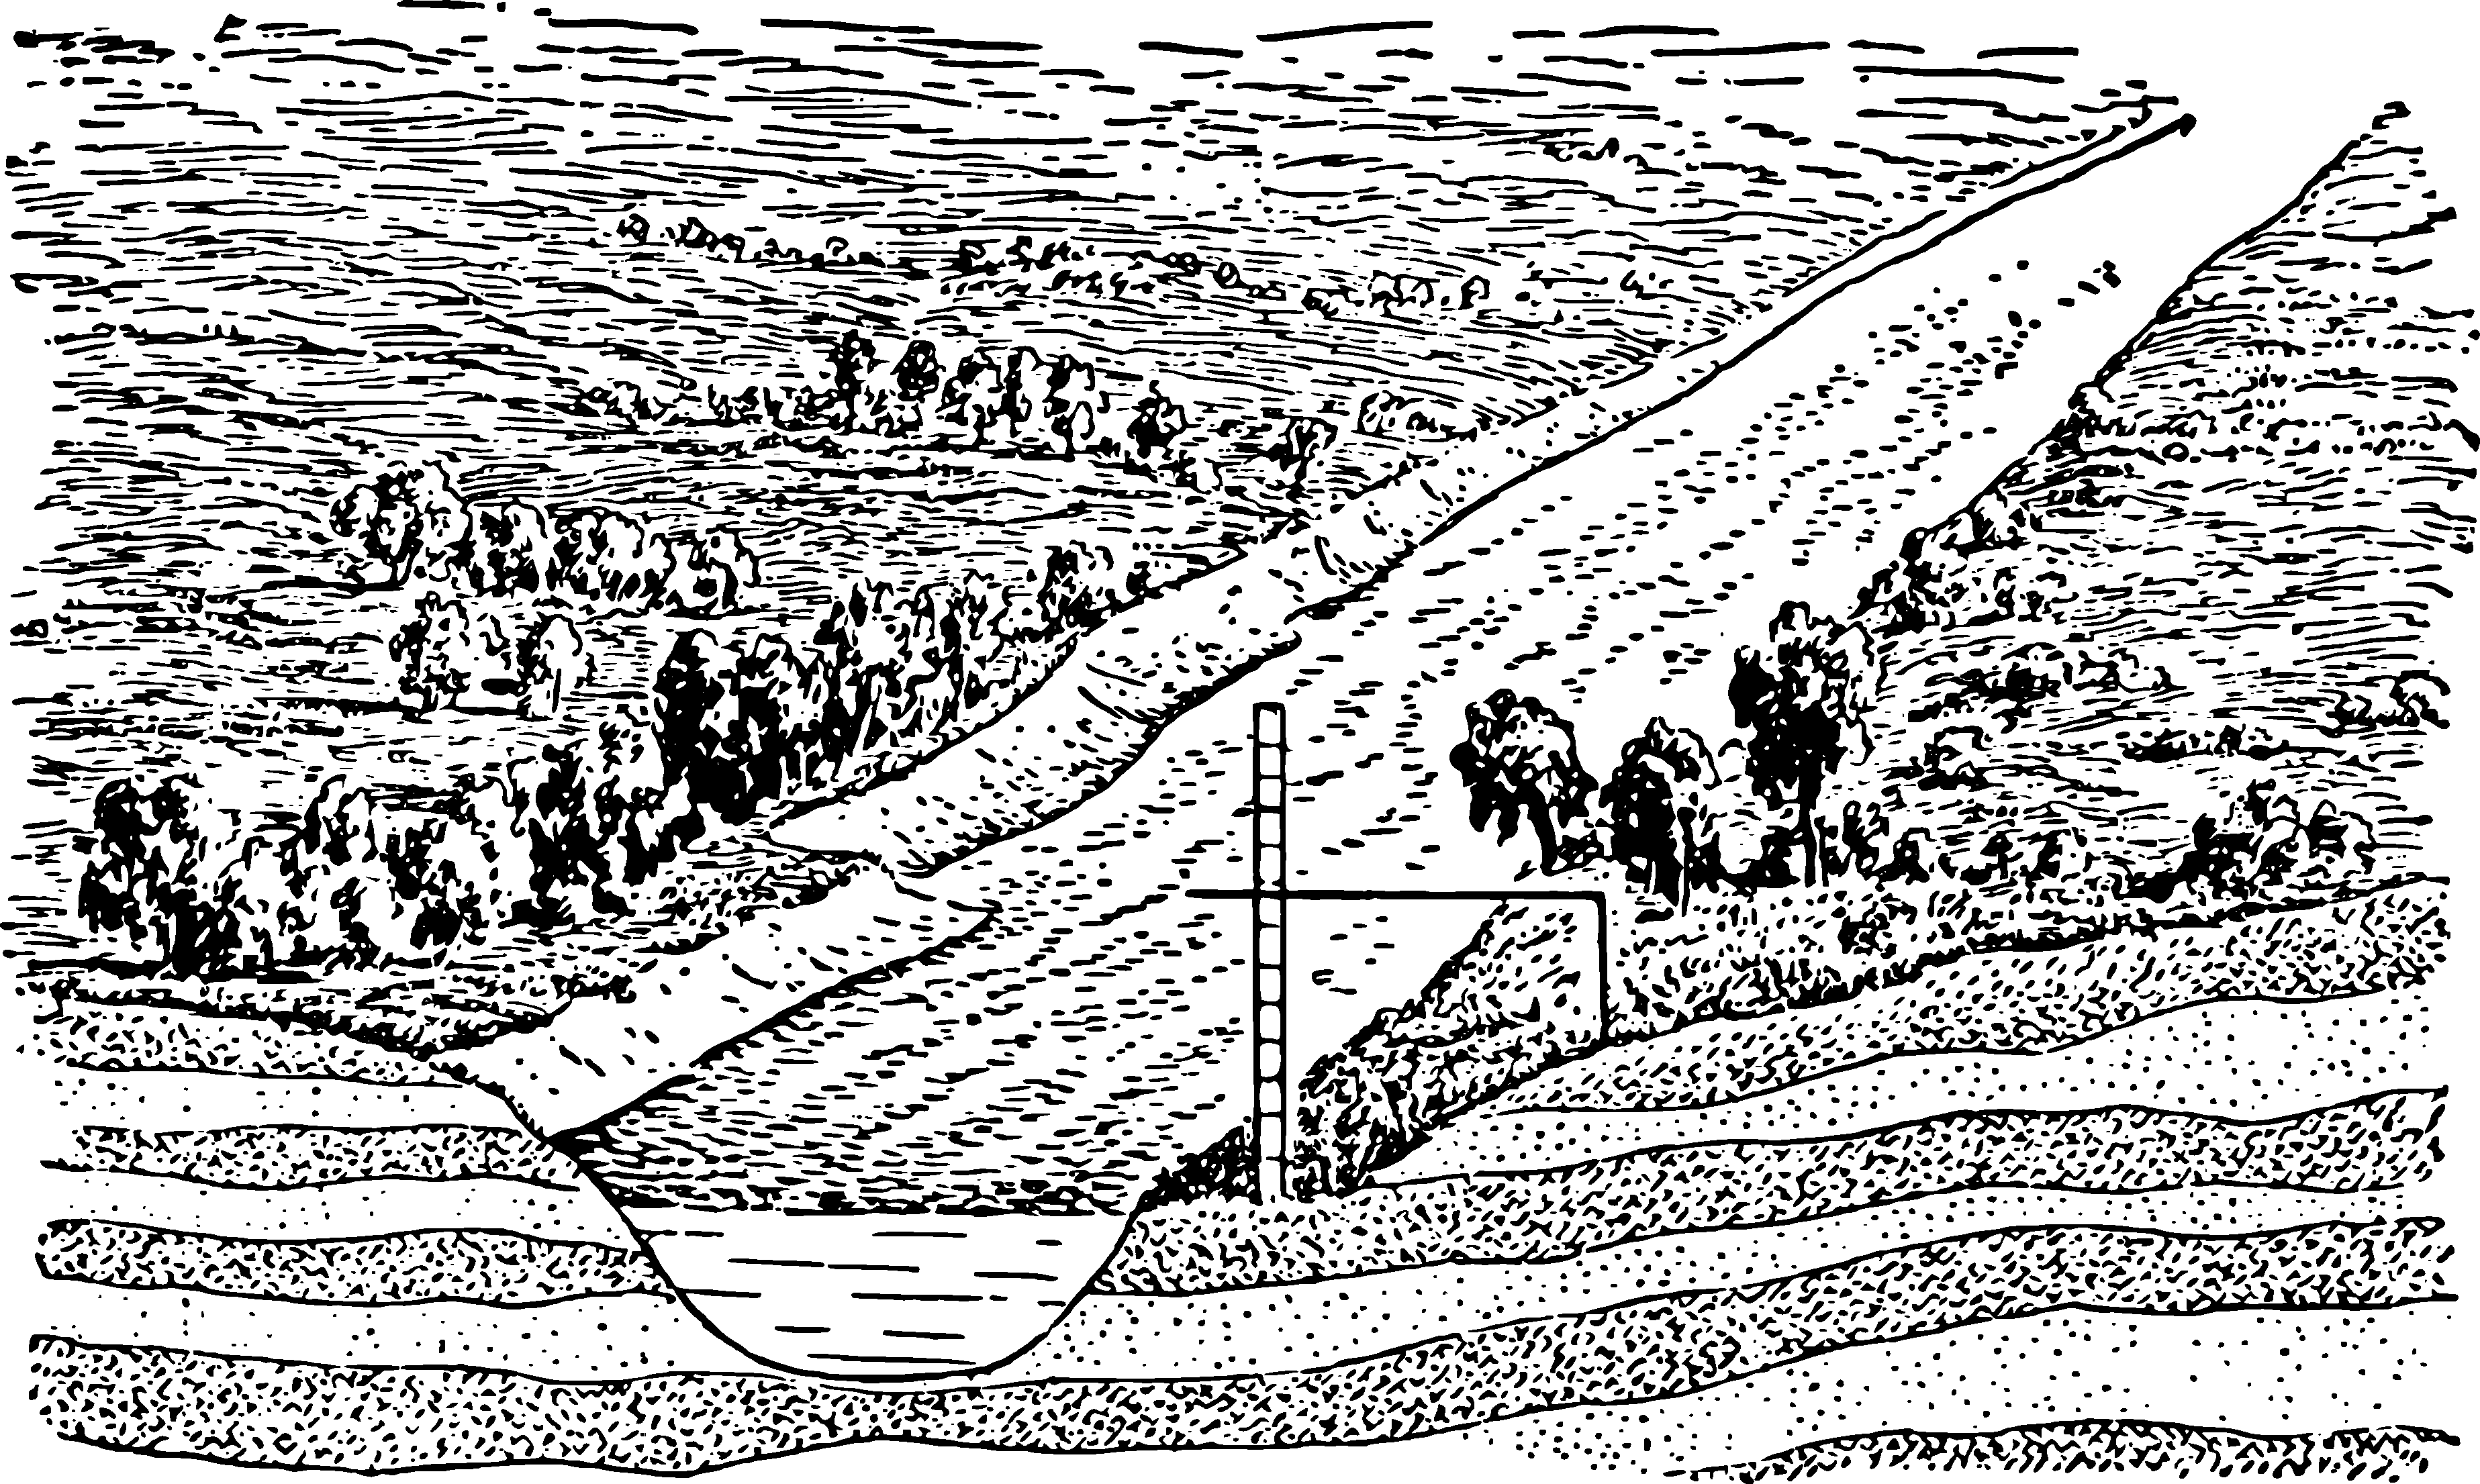
\includegraphics[width=\textwidth]{figures/ch-02/fig-044.pdf}
\sidecaption{Coast profile measurement.\label{fig-044}}
\end{figure}

Suppose the water level can be raised by the dam by 2.5 meters. In this case, you can estimate the potential power of your future hydroelectric power plant.

For this, energy experts recommend multiplying 1.4 (the second-by-second flow rate of the river) by 2.5 (the water level height) and by 6 (the coefficient, which varies depending on energy losses in machines). The result will be in kilowatts. Thus,
\begin{equation*}%
1.4 \times 2.5 \times 6 = 21\,\, \text{kilowatts}.
\end{equation*}
Since the river levels, and consequently the flow rates, vary throughout the year, it is necessary to calculate the value of the flow rate that is characteristic of the river for most of the year.

\section{Water Wheel}
\label{sec-2.09}

\ques A wheel with blades is installed near the bottom of the river so that it can rotate easily. In which direction will it rotate if the current is flowing from right to left (see \figr{fig-045})?

\begin{figure}[h!]
\centering
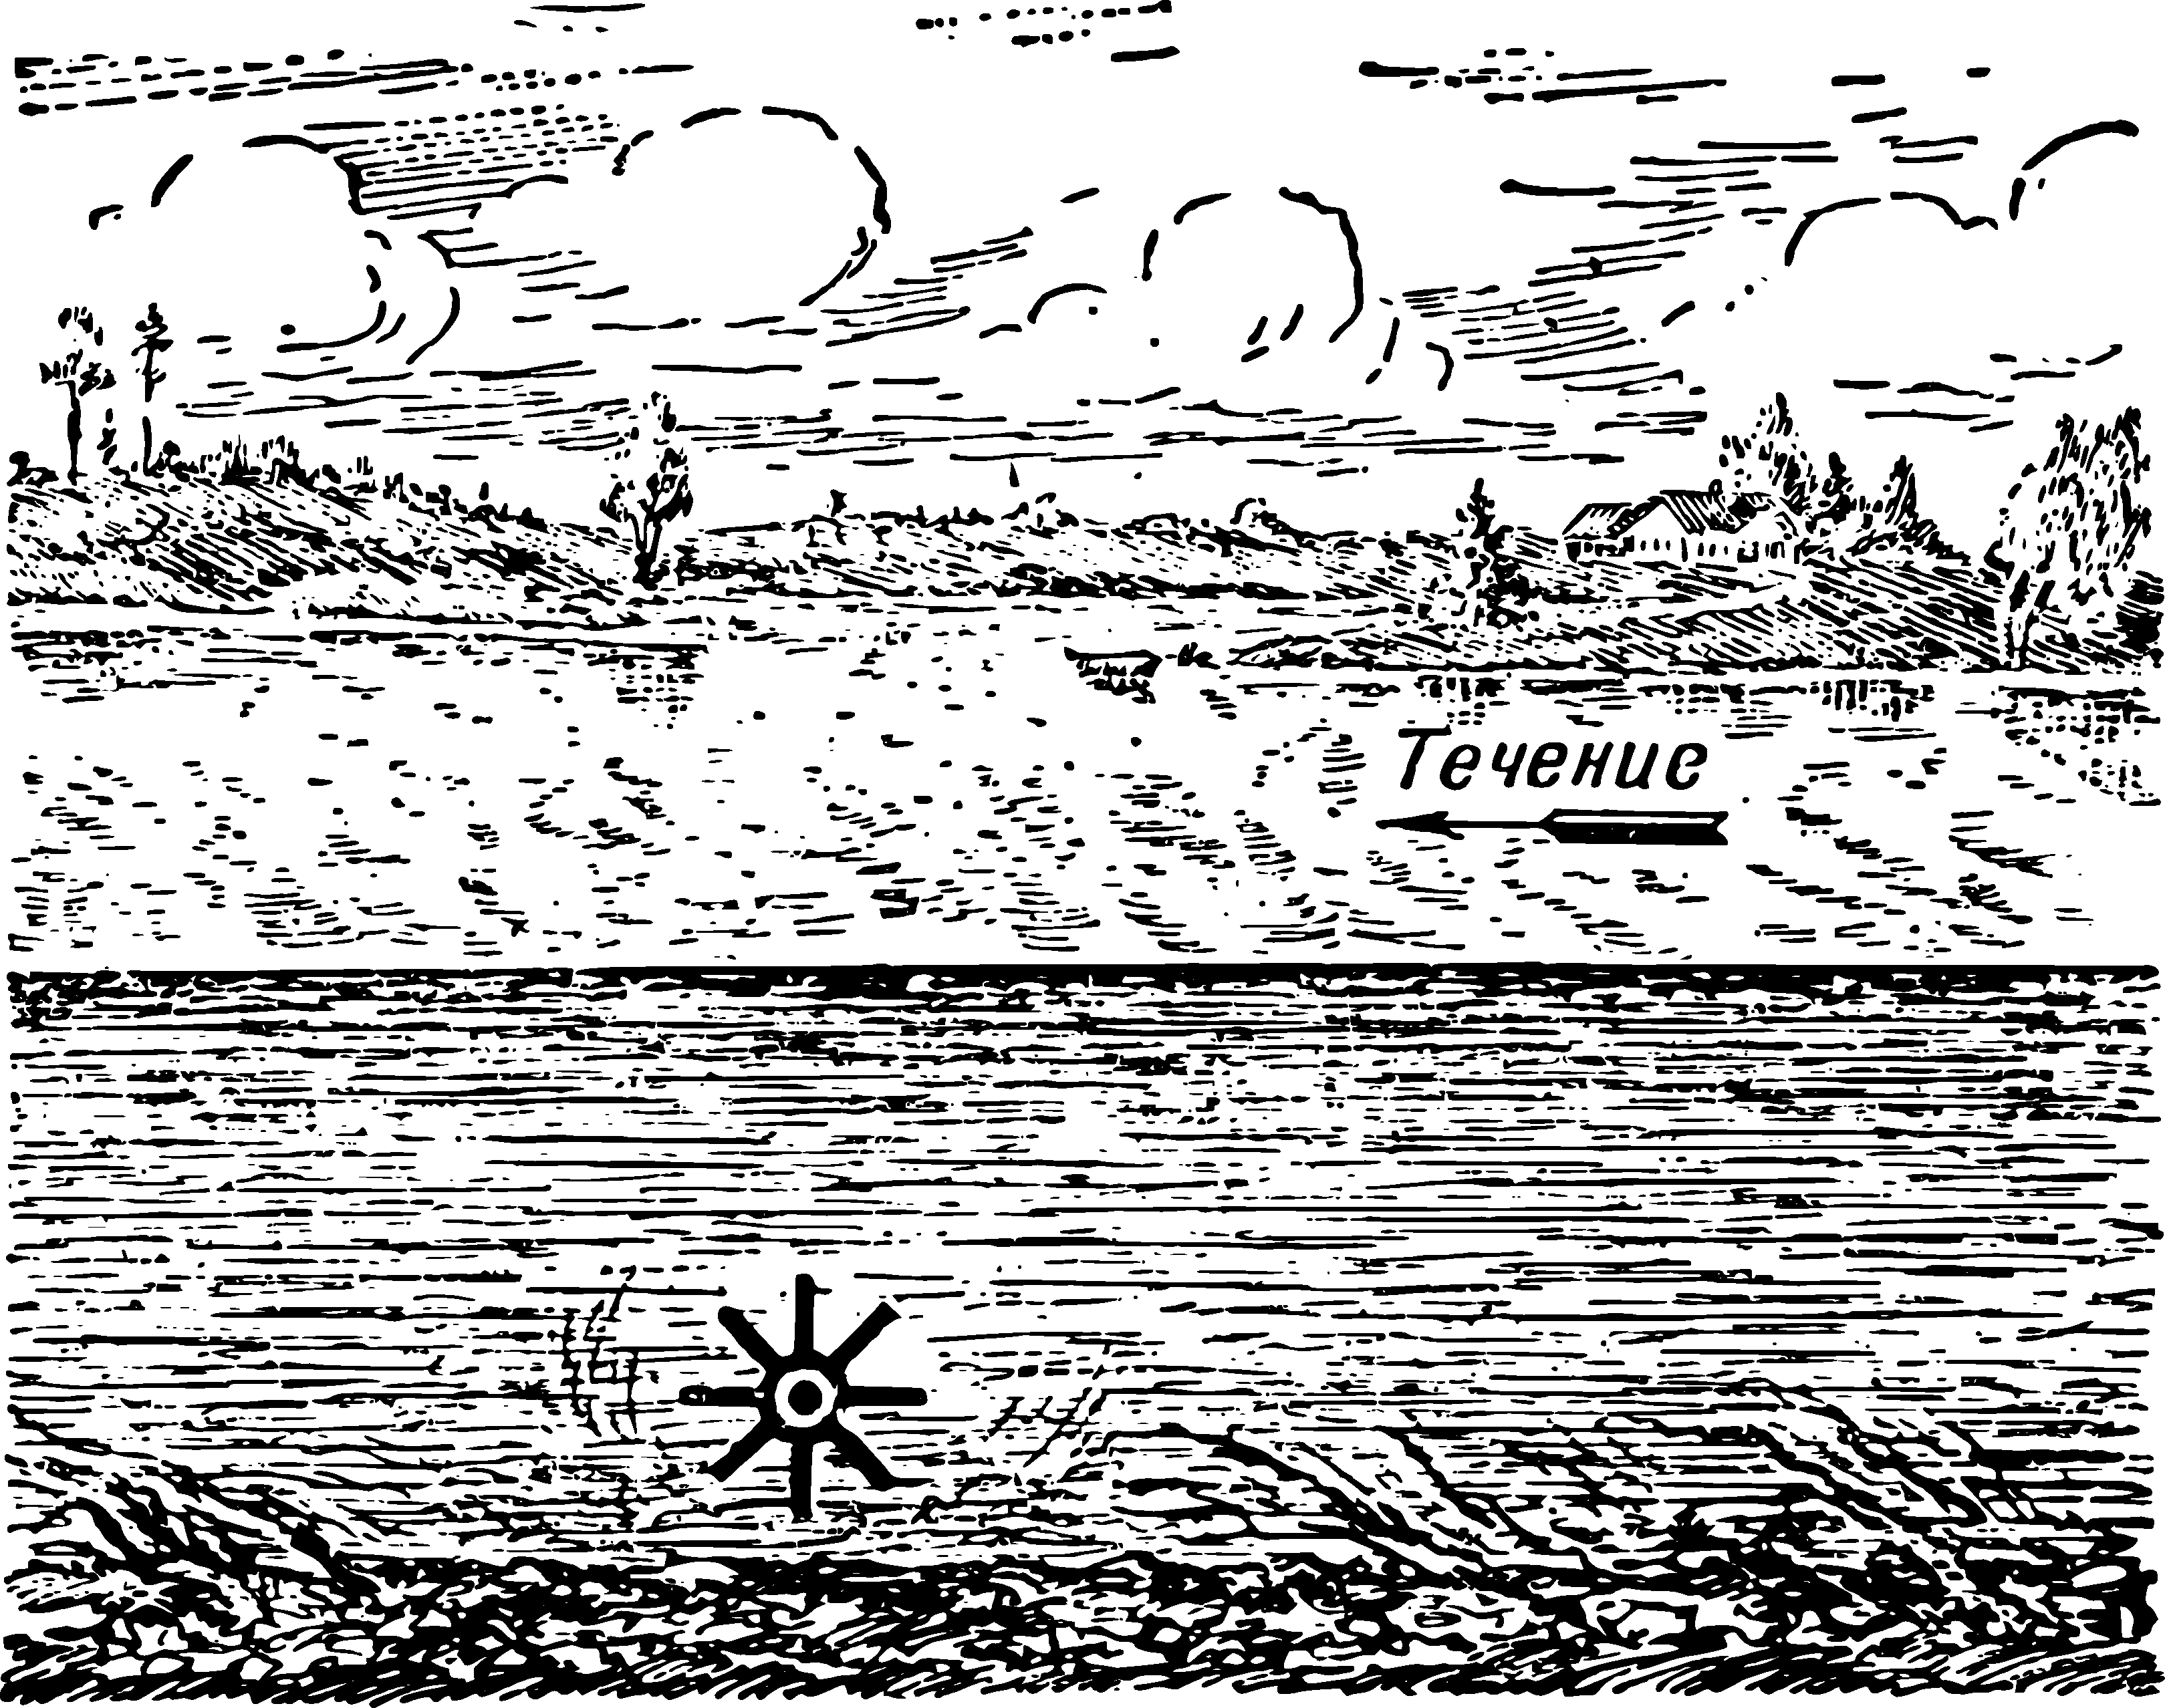
\includegraphics[width=\textwidth]{figures/ch-02/fig-045.pdf}
\sidecaption{In which direction will the wheel rotate?\label{fig-045}}
\end{figure}

\ans The wheel will rotate counterclockwise. The velocity of the deeper layers of water is lower than the velocity of the upper layers, therefore, the pressure on the upper blades will be greater than on the lower ones.


\section{Rainbow Film}
\label{sec-2.10}
On the river, into which water flows from the factory, you can often notice beautiful colourful iridescence near the outlet. Oil (for example, motor oil) flowing into the river along with the water from the plant remains on the surface as it is lighter and spreads out in an extremely thin layer. Can the thickness of such a film be measured or at least estimated?

The task seems intricate, but solving it is not particularly difficult. You already guess that we will not bother with the hopeless task of directly measuring the thickness of the film. We will measure it indirectly, in other words, calculate it.

Take a certain amount of motor oil, for example, 20 litres, and pour it onto the water, far from the shore (from a boat). When the oil spreads over the water in the form of a more or less clearly defined circular spot, measure the diameter of this circle at least approximately. Knowing the diameter, calculate the area. And since you also know the volume of the oil taken (it is easy to calculate by weight), then the thickness of the film will naturally be determined from here. Let's consider an example.


\ques One gram of kerosene, spreading over water, covers a circle with a diameter of 30 cm.\sidenote[][2cm]{The standard oil consumption for covering water bodies to destroy malaria mosquito larvae is 400 kilograms per hectare.} What is the thickness of the kerosene film on the water? One cubic centimetre of kerosene weighs 0.8 grams.

\ans Let's find the volume of the film, which is certainly equal to the volume of the kerosene taken. If one cubic centimetre of kerosene weighs 0.8 grams, then for 1 gram we have 
\begin{equation*}%
\frac{1}{0.8} = \SI{1.25}{\centi\meter\cubed} \qor \SI{1250}{\milli\meter\cubed}.
\end{equation*}
The area of the circle with a diameter of \SI{30}{\centi\meter}, or \SI{300}{\milli\meter}, is  \SI{70000}{\milli\meter\squared}. The desired thickness of the film is equal to the volume divided by the area of the base:
\begin{equation*}%
\frac{1250}{70000} = \SI{0.018}{\milli\meter}.
\si{\milli\meter\cubed}
\end{equation*}
In other words, less than \SI{0.02}{\milli\meter}. Direct measurement of such thickness using conventional means is, of course, impossible. Oil and soap films spread even thinner, reaching \SI{0.0091}{\milli\meter} or less. ``Once,'' recounts the English physicist Boys in the book \emph{Soap Bubbles}, ``I conducted such an experiment on a pond. A spoonful of olive oil was poured onto the water surface. Immediately a large spot was formed, about 20-30 meters in diameter. Since the spot was a thousand times longer and a thousand times wider than the spoon, the thickness of the oil layer on the water surface should have been approximately one millionth of the thickness of the oil layer in the spoon, or about 0.000002 millimetres.''


\section{Circles on the Water}
\label{sec-2.11}
\ques You've surely observed with curiosity the circles created by a stone thrown into calm water (see \figr{fig-046}). Explaining this instructive natural phenomenon has probably never been difficult for you: disturbance spreads from the point of origin in all directions at the same speed, so at any moment, all the points of disturbance must be equidistant from the source, forming circles.

\begin{figure}[h!]
\centering
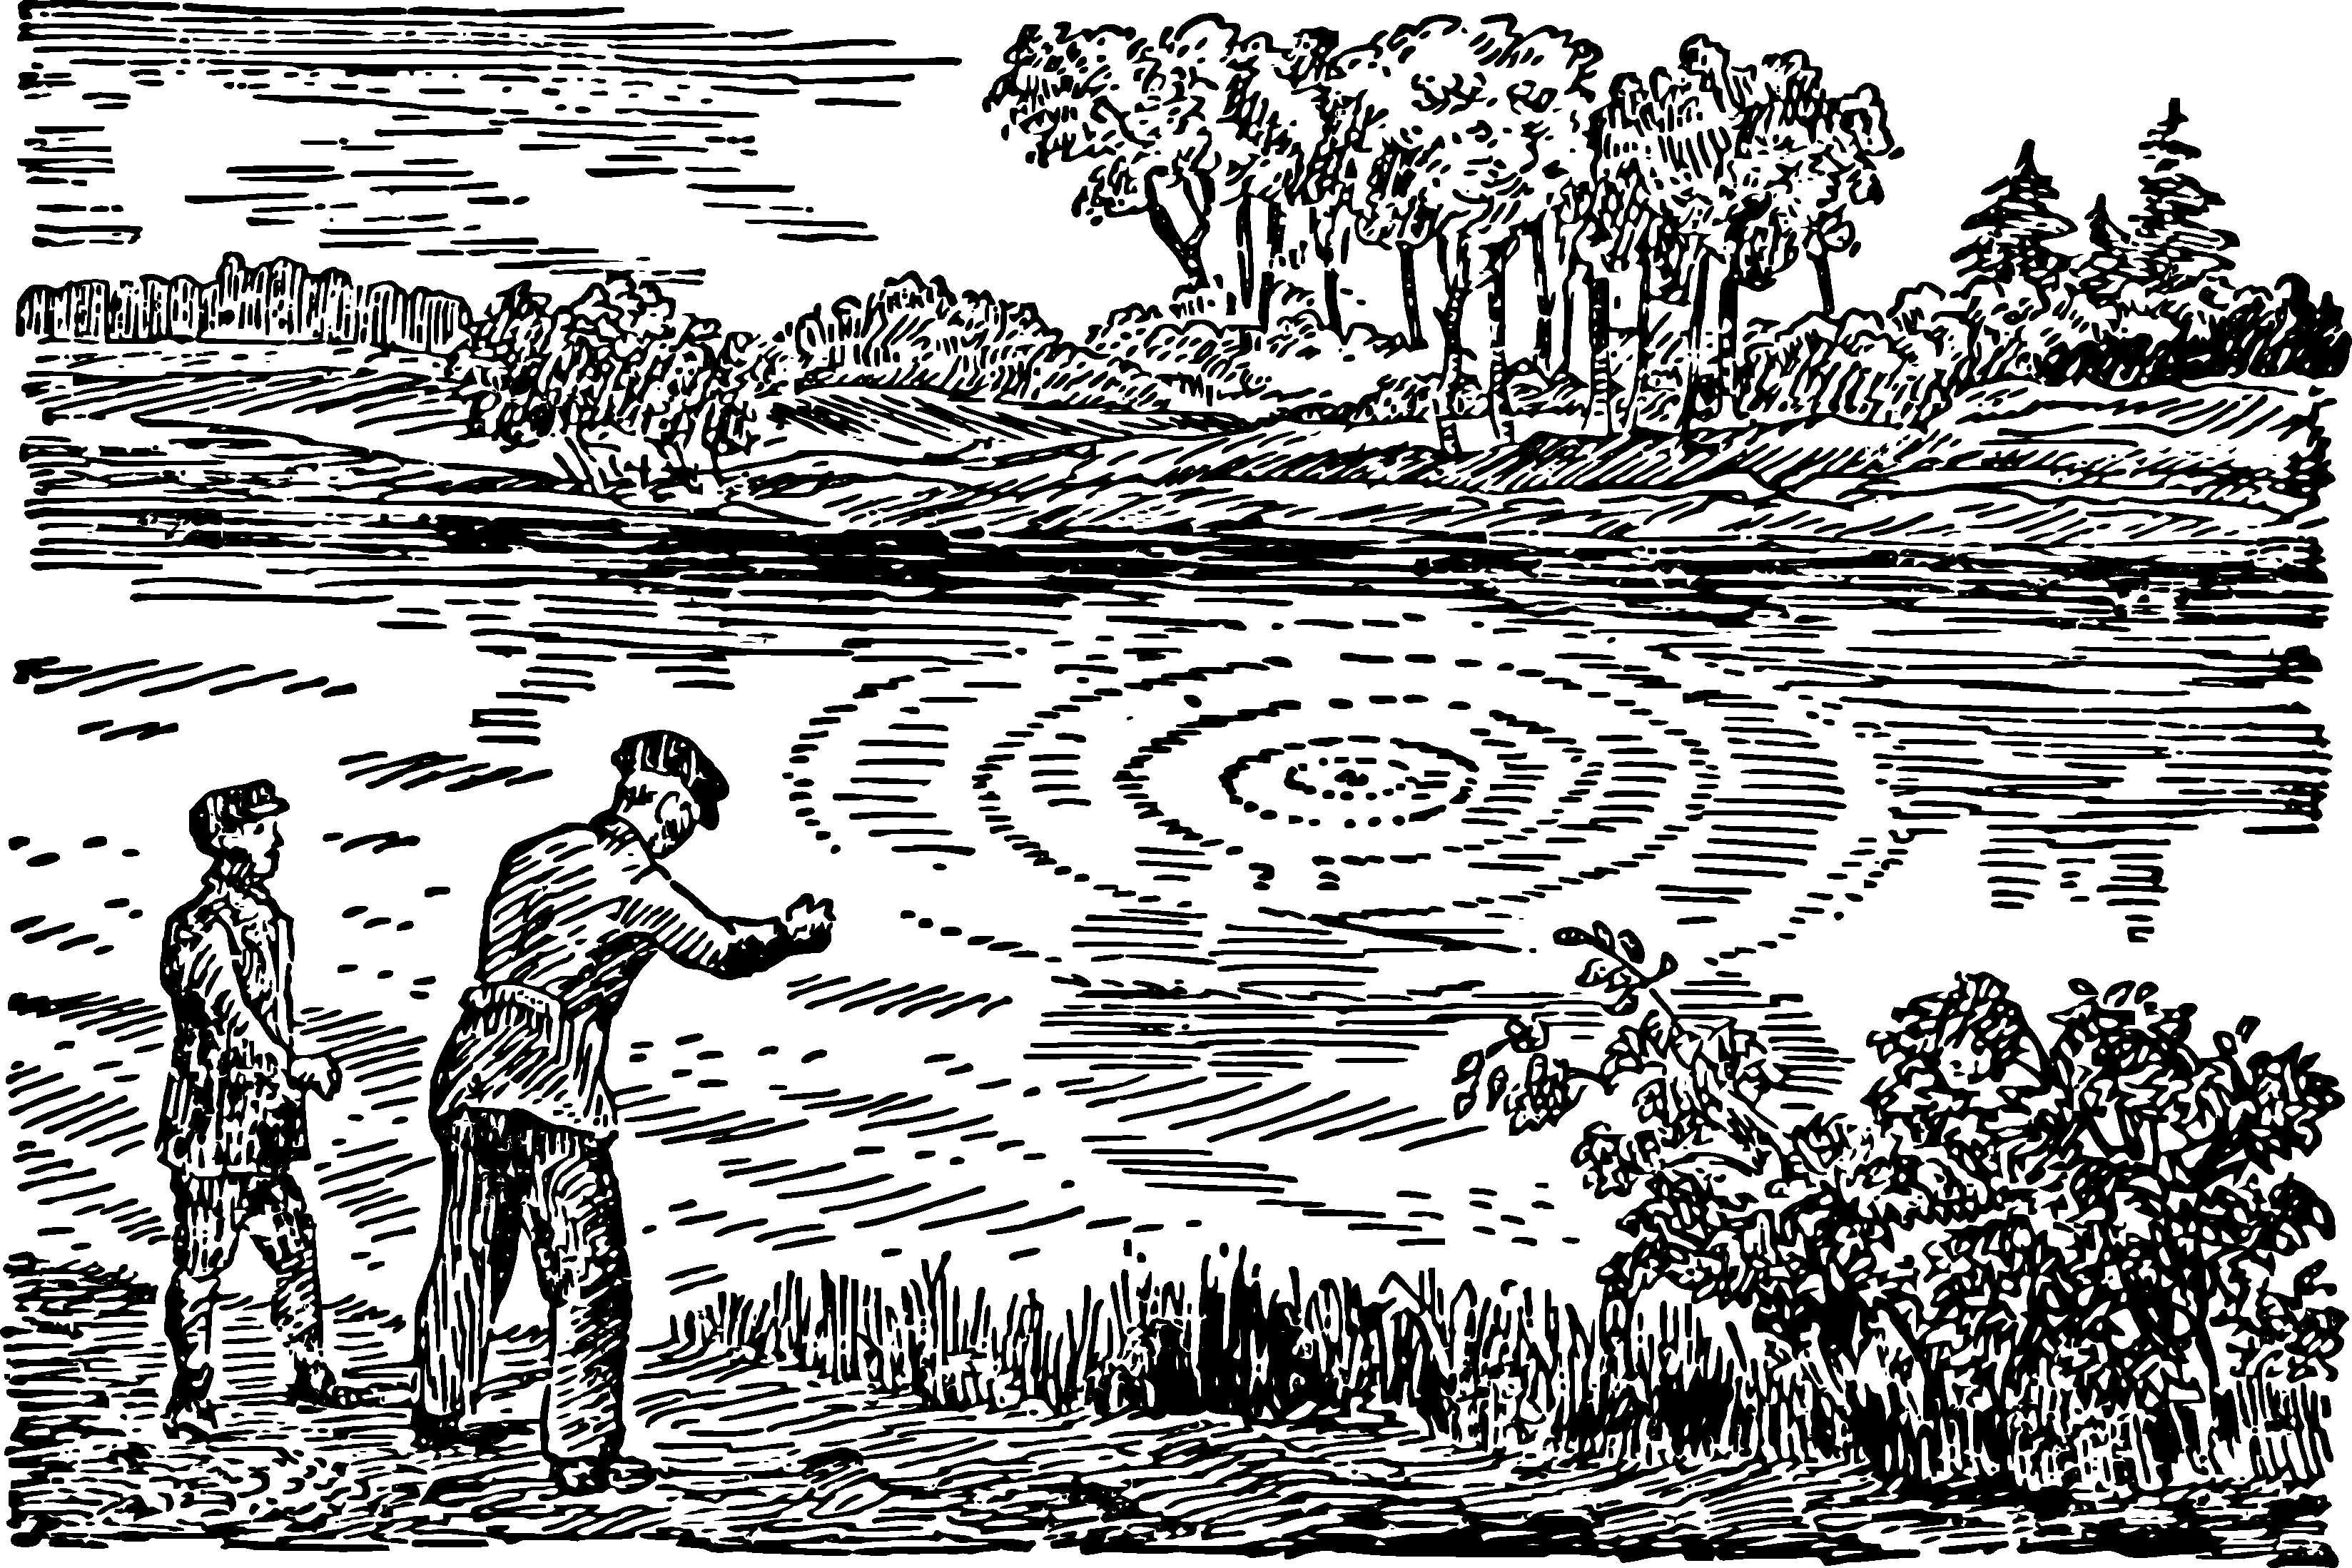
\includegraphics[width=\textwidth]{figures/ch-02/fig-046.pdf}
\sidecaption{Circles on the water.\label{fig-046}}
\end{figure}


But what about in flowing water? Should the waves from a stone thrown into a fast-flowing river also form circles, or will their shape be elongated?

At first glance, it might seem that in flowing water, circular waves should elongate in the direction of the current: the disturbance is transmitted downstream faster than upstream and sideways. Therefore, the disturbed parts of the water surface should, it seems, arrange themselves along some elongated closed curve, at least not in a circle.

However, in reality, this is not the case. By throwing stones into the swiftest river currents, you can see that the waves formed are strictly circular -- exactly the same as in still water. Why is this?

\begin{figure}[h!]
\centering
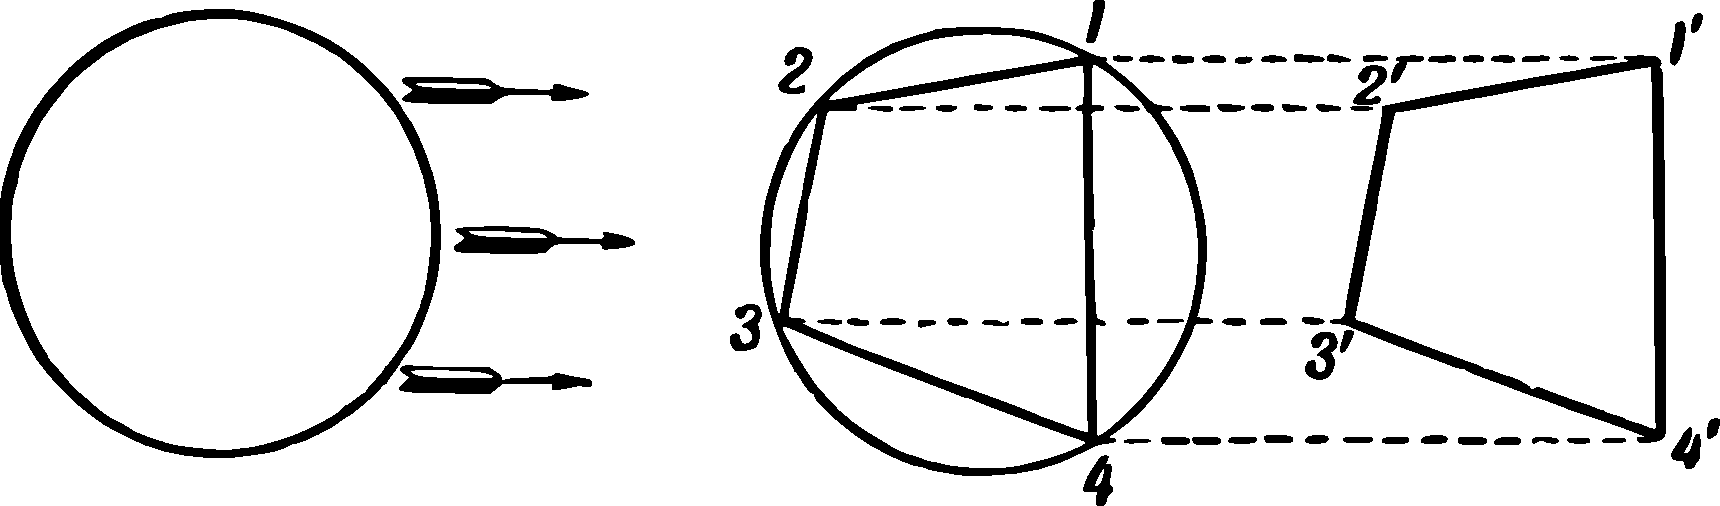
\includegraphics[width=\textwidth]{figures/ch-02/fig-047.pdf}
\sidecaption[][-1.5cm]{The flow of water does not change the shapes of the waves.\label{fig-047}}
\end{figure}

\ans Let's reason as follows. If the water were not flowing, the waves would be circular. What change does the flow introduce? It carries each point of this circular wave in the direction indicated by the arrows (see \figr{fig-047}, left), and all points are moved along parallel lines at the same speed, i.e., the same distance. And ``parallel displacement'' (translation) does not change the shape of the figure. Indeed, as a result of such displacement, point $\mathit{1}$ (\figr{fig-047}, right) will be at point $\mathit{1'}$, point $\mathit{2}$ will be at point $\mathit{2'}$, and so on; quadrilateral $\mathit{1234}$ will be replaced by quadrilateral $\mathit{1'2'3'4'}$, which is equal to it, as can be easily seen from the formed parallelograms $\mathit{122'1'}$, $\mathit{233'2'}$, $\mathit{344'3'}$, and so on. By taking not just four but more points on the circumference, we would also get equal polygons; finally, by taking an infinite number of points, i.e., a circle, we would get an equal circle after parallel displacement.

That's why the downstream movement of water does not change the shapes of the waves -- they remain circular even in flowing water. The difference is only that on the surface of a lake, the circles do not move (if we don't consider that they diverge from their stationary centre), while on the surface of a river, the circles move together with their centre at the speed of the water flow.

\section{Fantastic Shrapnel}
\label{sec-2.12}
\ques Let's tackle a problem that seems unrelated at first but, as we will see, is closely related to the topic at hand.

Imagine a shrapnel projectile flying high in the air. It begins to descend and suddenly explodes; the fragments scatter in different directions. Let's assume that all of them are thrown by the explosion with the same force and travel without encountering any obstacles from the air. The question is: how will the fragments be arranged one second after the explosion if during this time they have not yet reached the ground?

\ans The problem resembles the problem of circles on water. And here it seems that the fragments should be arranged in a shape elongated downwards, in the direction of descent; after all, the fragments thrown upwards fly slower than those thrown downwards. However, it is easy to prove that the fragments of our imaginary shrapnel should be arranged on the surface of a sphere. Let's momentarily imagine that there is no gravity; then, of course, all fragments will fly from the explosion site to the same distance within a second, i.e., they will be arranged on the surface of a sphere. Now let's introduce the force of gravity. Under its influence, the fragments should descend; but since all bodies, as we know, fall at the same speed, the fragments should descend to the same distance within a second, along parallel lines.\sidenote{The differences are due to the air resistance, which we have excluded in our task.} But such parallel displacement does not change the shape of the figure—the sphere remains a sphere.

So, the fragments of the fantastic shrapnel should form a sphere, which, as if inflating, descends downward at the speed of a freely falling body.

\section{The Keel Wave}
\label{sec-2.13}

Let's return to the river. (Standing on a bridge, pay attention to the wake left by a fast-moving boat. You will see how two water crests diverge at an angle from the bow (see \figr{fig-048}). Where do they come from? And why is the angle between them sharper the faster the boat moves?

\begin{figure}[h!]
\centering
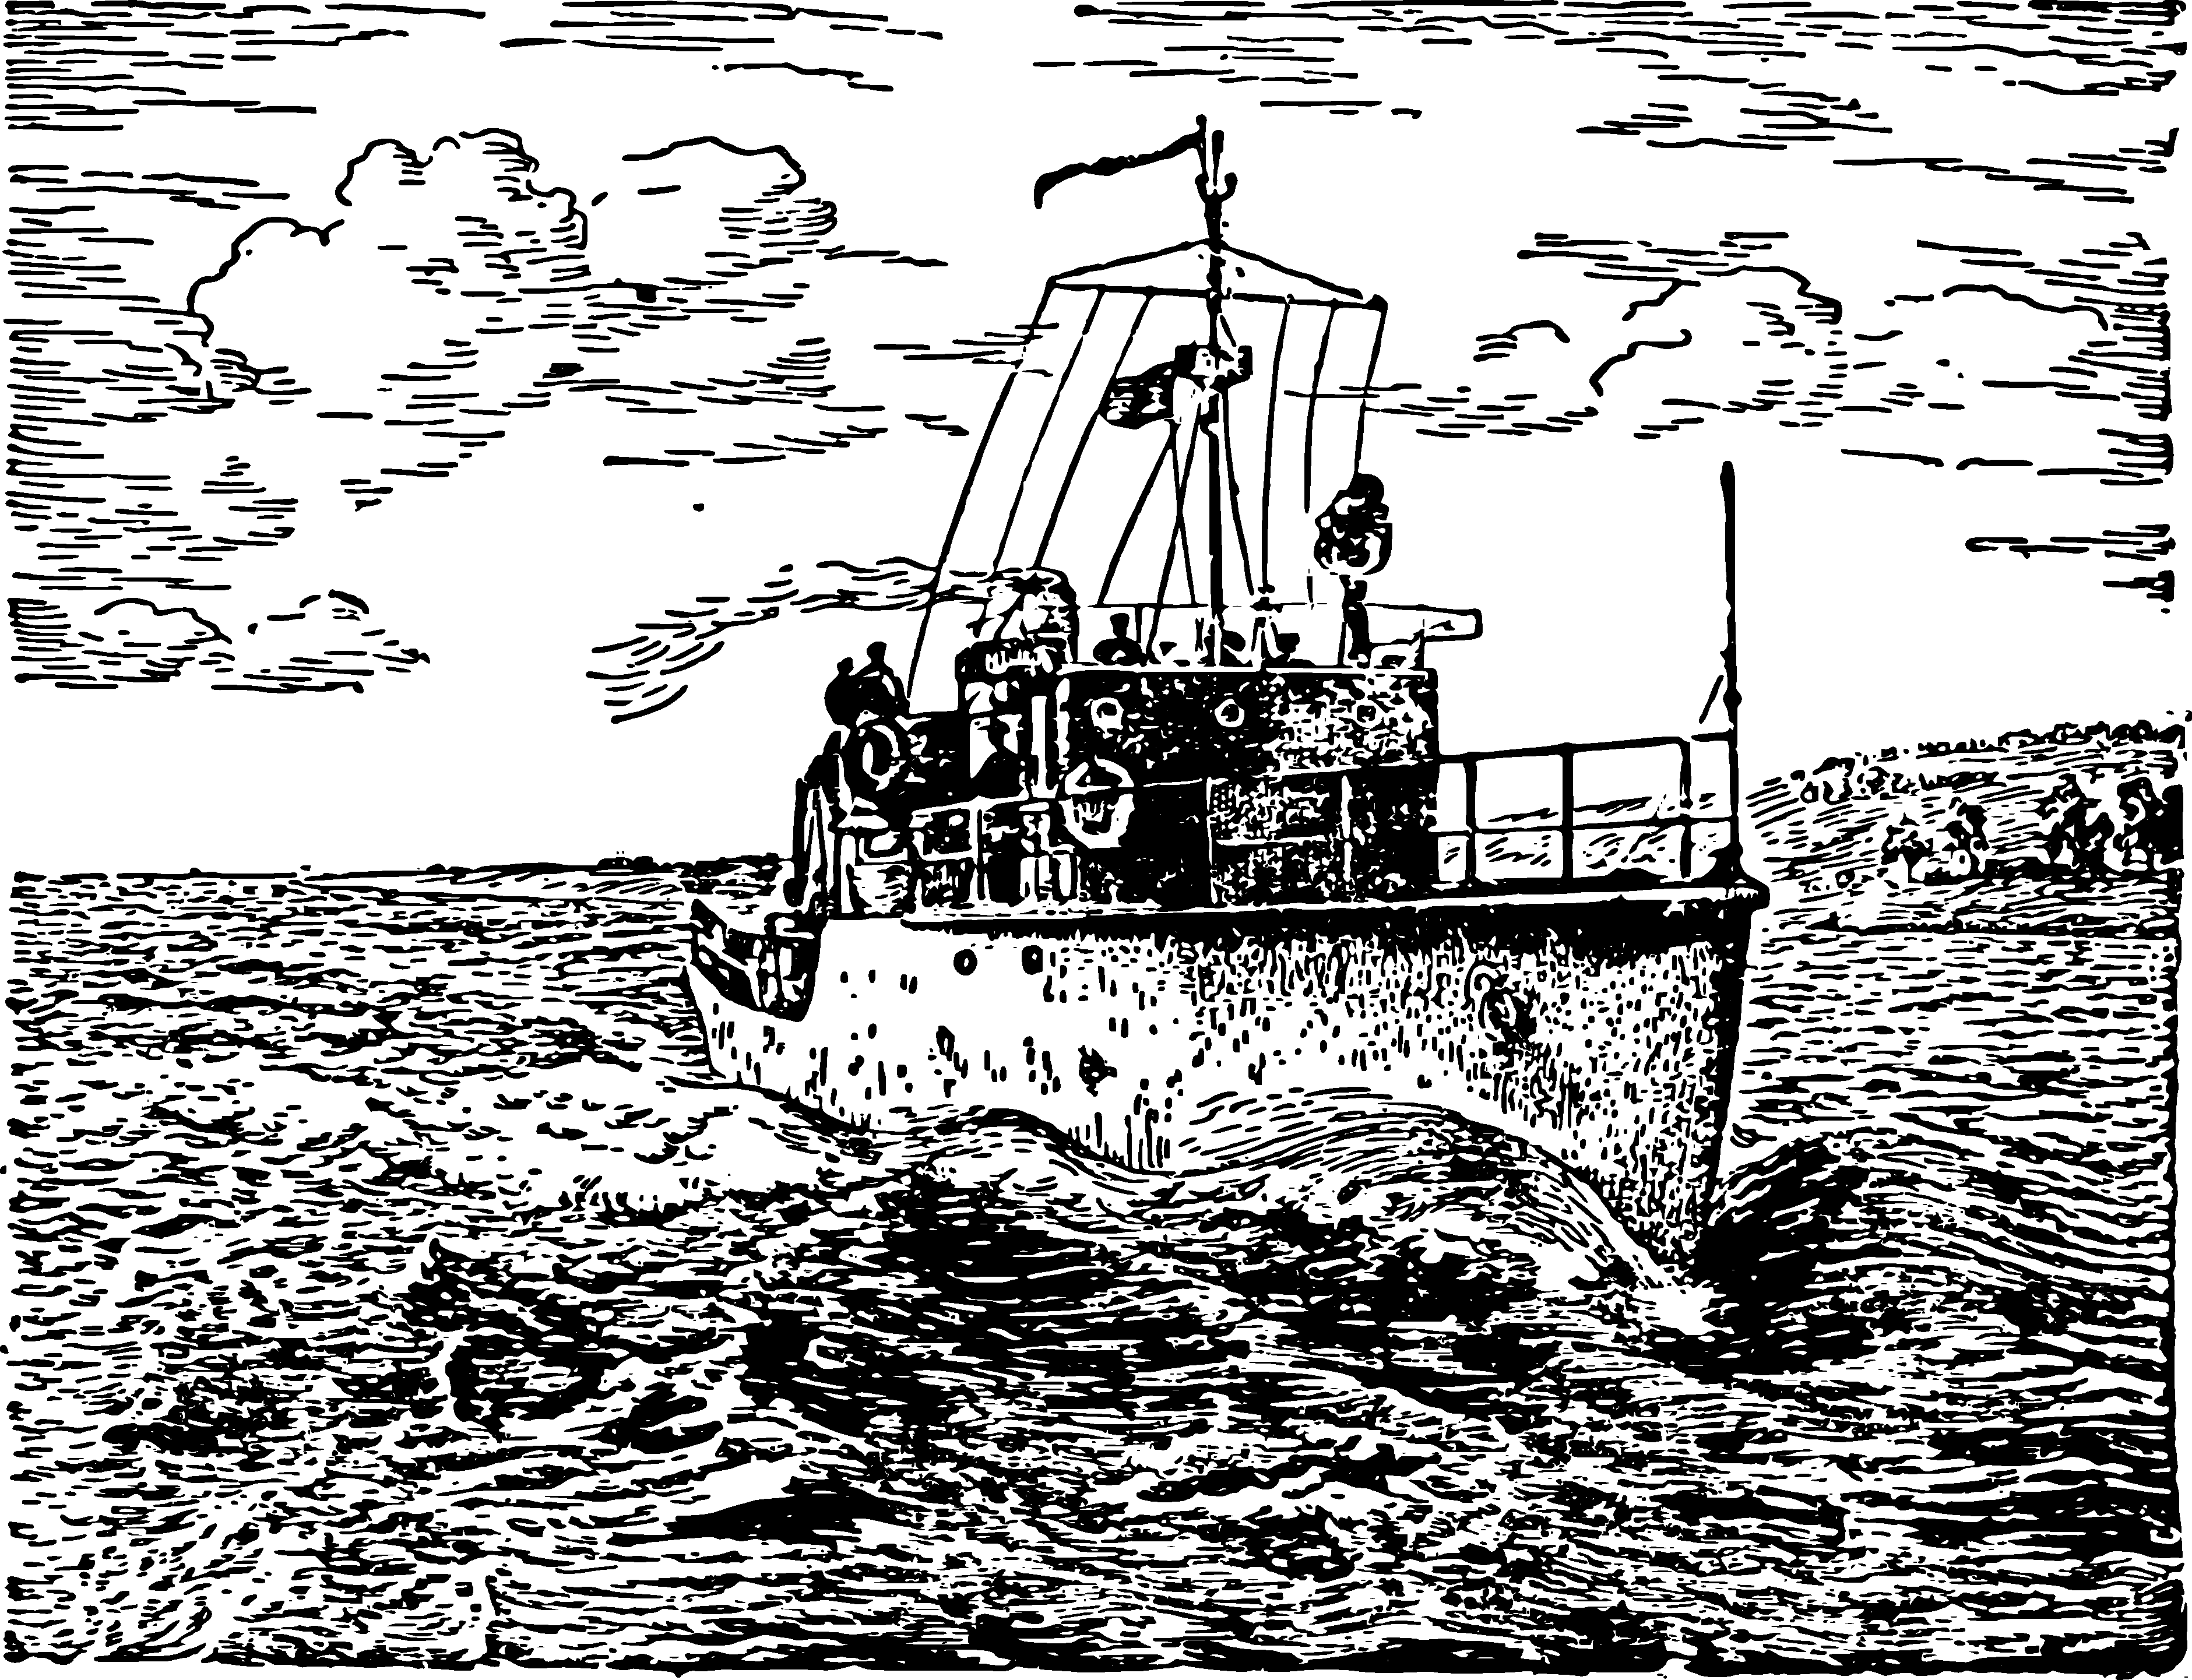
\includegraphics[width=\textwidth]{figures/ch-02/fig-048.pdf}
\sidecaption{The keel wave.\label{fig-048}}
\end{figure}
To understand the reason for the emergence of these crests, let's once again turn to the diverging circles formed on the water surface by stones thrown into it. By throwing stones into the water at certain intervals, you can see circles of different sizes on the water surface; the later a stone is thrown, the smaller the circle it creates. 

If you throw stones along a straight line, the circles formed collectively generate a wave similar to the one at the bow of a ship. The smaller and more frequent the stones are thrown, the more noticeable the similarity becomes. By immersing a stick in the water and moving it along the water surface, you effectively replace the intermittent falling of stones with continuous motion, and then you see exactly the wave that forms at the bow of a ship. To make this vivid picture even clearer, let's add a bit more. 

Each moment, the bow of the ship, plunging into the water, generates the same circular wave as a thrown stone. The circle expands in all directions, but meanwhile, the ship moves forward and creates a second circular wave, followed immediately by a third, and so on. The intermittent formation of circles caused by stones is perceived as continuous due to their continuous occurrence, resulting in the pattern shown in \figr{fig-049}.

Meeting each other, the crests of neighbouring waves break each other: only two small segments of the complete circle remain intact, which are located on their outer parts. These outer segments merge to form two continuous crests, positioned as external tangents to all circular waves (\figr{fig-049}, right).


\begin{figure}[h!]
\centering
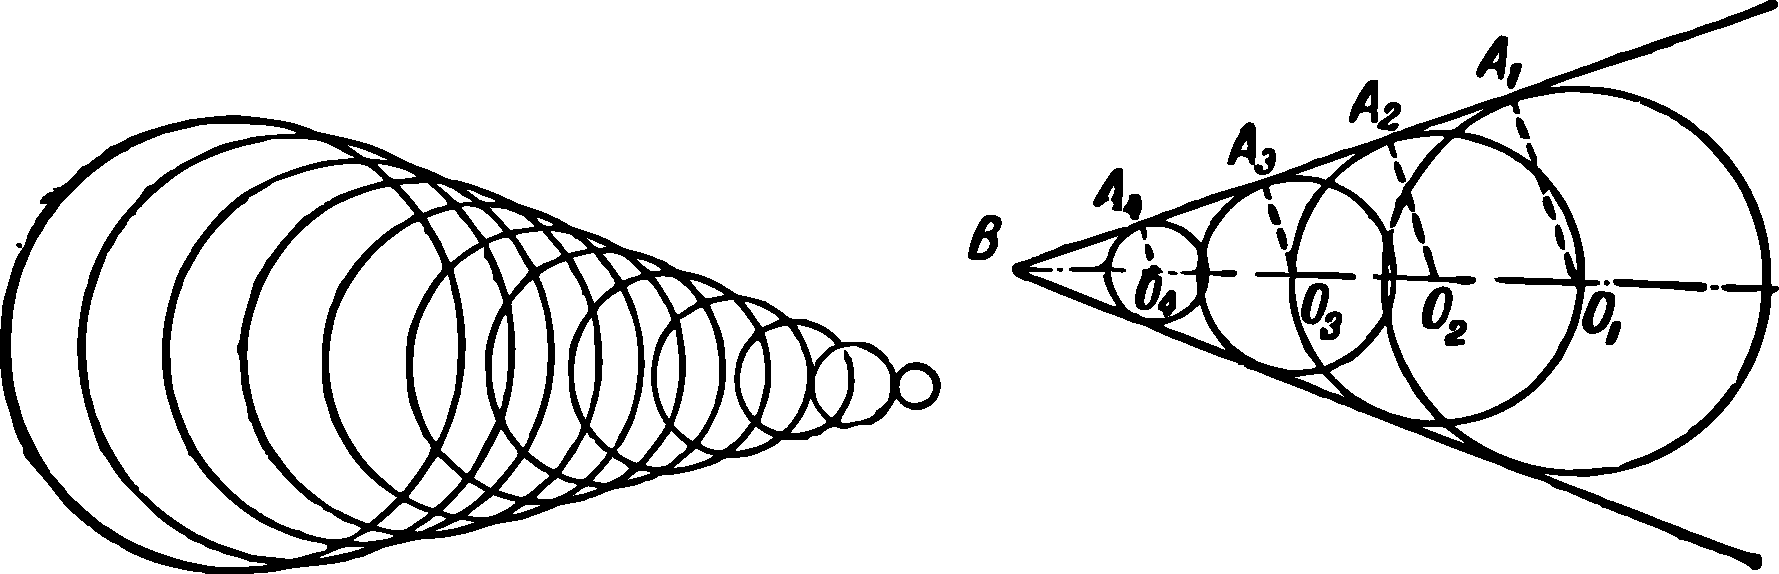
\includegraphics[width=\textwidth]{figures/ch-02/fig-049.pdf}
\sidecaption{How the keel wave is formed.\label{fig-049}}
\end{figure}

This is how the origin of the water crests visible behind the boat, behind any body moving rapidly along the water surface, occurs.

It follows directly from this that this phenomenon is possible only when the body moves faster than the water waves. If you slowly move a stick through the water, you will not see any crests: the circular waves will be arranged one inside the other, and it will be impossible to draw a common tangent to them.

Diverging crests can also be observed when the body stands still and the water flows past it. If the current of the river is fast enough, such wakes are formed in the water flowing around bridge piers. The shape of the waves is even more distinct here than, for example, from a steamship, as their regularity is not disrupted by the action of a propeller.

Having clarified the geometric aspect of the matter, let's try to solve such a problem.

\ques What determines the magnitude of the angle between both branches of the keel wave of the steamer?

\ans The angle between the branches of the keel wave of a steamship depends on several factors, primarily the speed of the ship relative to the speed of the wave propagation in the water.

Let's draw radii from the centre of the circular waves (\figr{fig-49}, right) to the corresponding points of the straight wave crest, i.e., to the points of common tangency. It's easy to understand that $O_{1}B$ represents the distance travelled by the ship's bow in some time, and $O_{1}A_{1}$ -- represents the distance over which the wave propagates in the same time period. The ratio $O_{1}B/O_{1}A_{1}$ is the sine of angle $O_{1}BA_{1}$, which, in turn, is the ratio of the wave propagation velocity to the ship's velocity. Therefore, the angle $B$ between the crests of the keel wave is nothing else but twice the angle whose sine is the ratio of the wave propagation velocity to the ship's velocity.


The speed of wave propagation in water is approximately the same for all vessels. Therefore, the angle between the branches of the keel wave primarily depends on the speed of the ship. In general, the sine of half the angle is proportional to this speed. Conversely, the angle's magnitude indicates how many times the ship's speed exceeds the speed of the waves. For instance, if the angle between the branches of the keel wave is \ang{30}, as is common for most cargo and passenger ships, then the sine of half this angle (approximately 0.26) suggests that the ship's speed exceeds the wave speed by roughly four times.

\section{Speed of Projectiles}
\label{sec-2.14}
\begin{marginfigure}%[-3cm]%[h!]
\centering
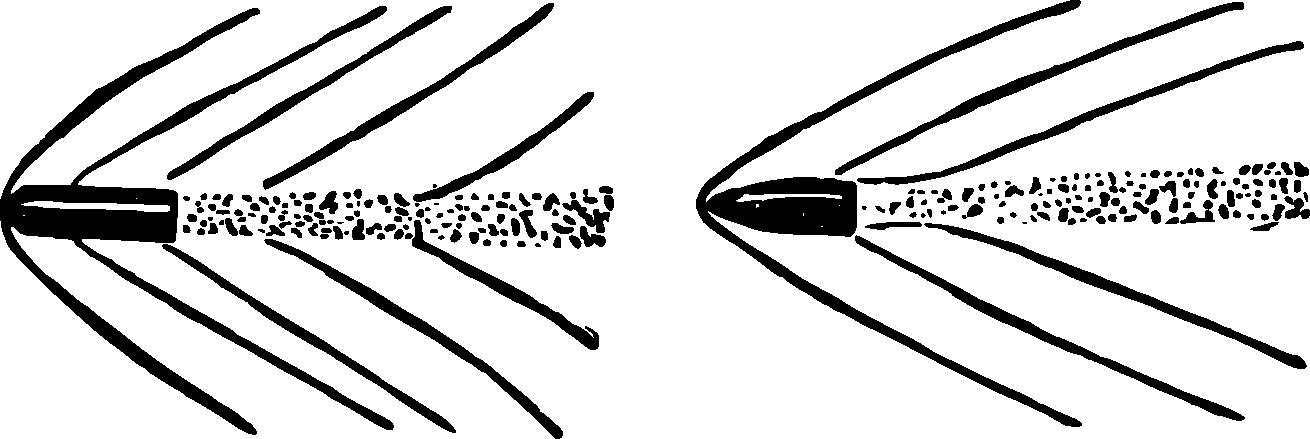
\includegraphics[width=0.6\textwidth]{figures/ch-02/fig-050.pdf}
\sidecaption{A head wave (shock wave) in the air formed by a flying projectile.\label{fig-050}}
\end{marginfigure}

\begin{marginfigure}[3cm]%[h!]
\centering
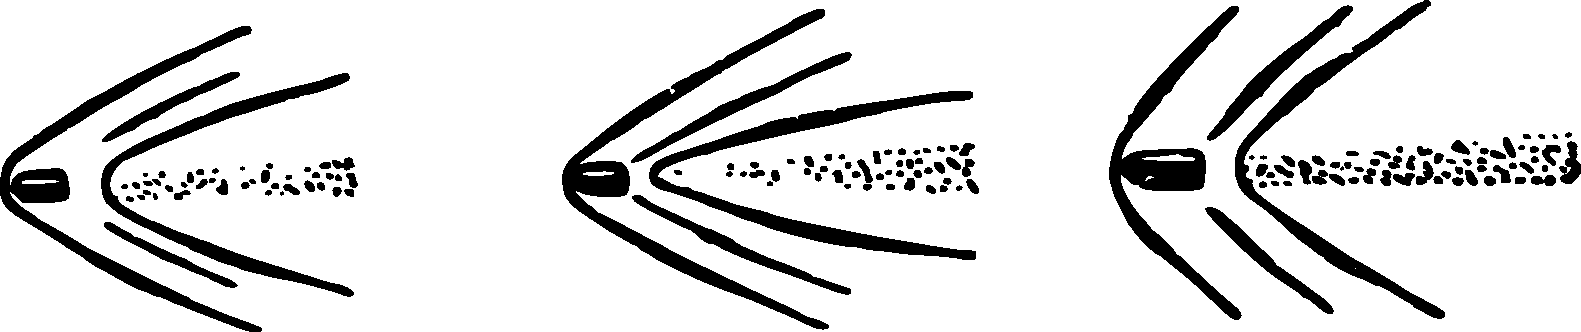
\includegraphics[width=0.6\textwidth]{figures/ch-02/fig-051.pdf}
\sidecaption{Another example of head wave (shock wave) in the air formed by a flying projectile.\label{fig-051}}
\end{marginfigure}

\ques Waves, similar to those considered now, are generated in the air by a flying bullet or artillery shell.

There are methods to photograph a projectile in flight; \figr{fig-050} and \figr{fig-051} reproduce two such images of projectiles moving at different speeds. In both drawings, the ``head wave''\sidenote[][4cm]{The term shock wave is commonly used now. \textsc{dm}} that interests us is clearly visible (as it is called in this case). Its origin is the same as that of the bow wave of a ship. And here the same geometric relationships apply, namely: the sine of half the angle of divergence of the head waves is equal to the ratio of the speed of wave propagation in the air to the speed of the projectile itself. But wave propagation in the air occurs at a speed close to the speed of sound, i.e., \SI{330}{\meter\per\second}. Therefore, it is easy, having a photograph of a flying projectile, to approximately determine its speed. How to do this for the two images provided here?

\ans Let's measure the angle of divergence of the head wave branches in \figr{fig-050} and \figr{fig-051}. In the first case, it is about \ang{80}, and in the second case -- approximately \ang{55}. Half of them are \ang{40} and \ang{27.5}. For \ang{40}, $\sin(\ang{40}) = 0.64$, and for \ang{27.5}, $\sin(\ang{27.5}) = 0.46$. Therefore, the speed of wave propagation in the air, i.e., \SI{330}{\meter\per\second}, is 0.64 of the projectile's flight speed in the first case and 0.46 in the second. Hence, $330 / 0.64 = \SI{520}{\meter\per\second}$ for the speed of the first projectile, and $330 / 0.46 = \SI{720}{\meter\per\second}$ for the speed of the second projectile.

You see that quite simple geometric considerations, with some support from physics, helped us solve a problem that, at first glance, seemed very intricate; to determine the speed of a projectile at the moment of photography. (However, this calculation is only approximately correct, since some secondary circumstances are not taken into account here.)

For those who want to independently perform such a speed calculation for projectiles, here are three reproductions of photographs of shells flying at different speeds (\figr{fig-052}).

\begin{figure}[h!]
\centering
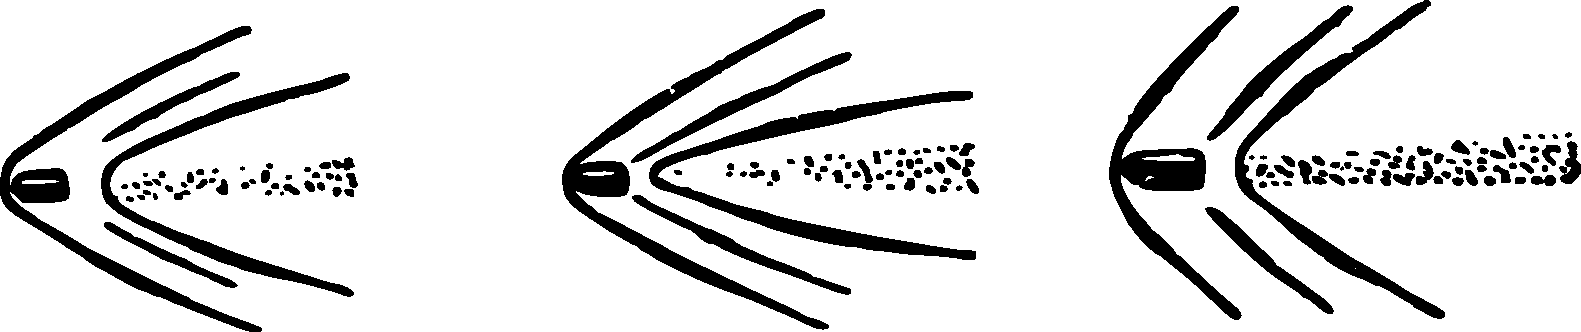
\includegraphics[width=\textwidth]{figures/ch-02/fig-052.pdf}
\sidecaption{How to determine the speed of flying projectiles?\label{fig-052}}
\end{figure}

\section{Finding Pond Depth}
\label{sec-2.15}

The ripples on the water distracted us for a while in the field of artillery. Let's go back to the river again and consider the Hindu lotus problem,

The ancient Hindus had a custom of offering tasks and rules in verse, Here is one of such tasks:

\ques 
\begin{quote}
\emph{
Above the tranquil lake, \\
With a half-foot size, the lotus flower rose. \\
It grew alone. And the wind, in a gust, \\
Bent it sideways. \\
No more flower above the wave, \\
But the fisherman found it, in early spring, \\
Two feet from where it grew.\\
So, I propose a question: \\
How deep is the water of the lake?}\\[-15pt]
\flushright{Translated by  \emph{V. I. Lebedev}}
\end{quote}

\begin{figure}[h!]
\centering
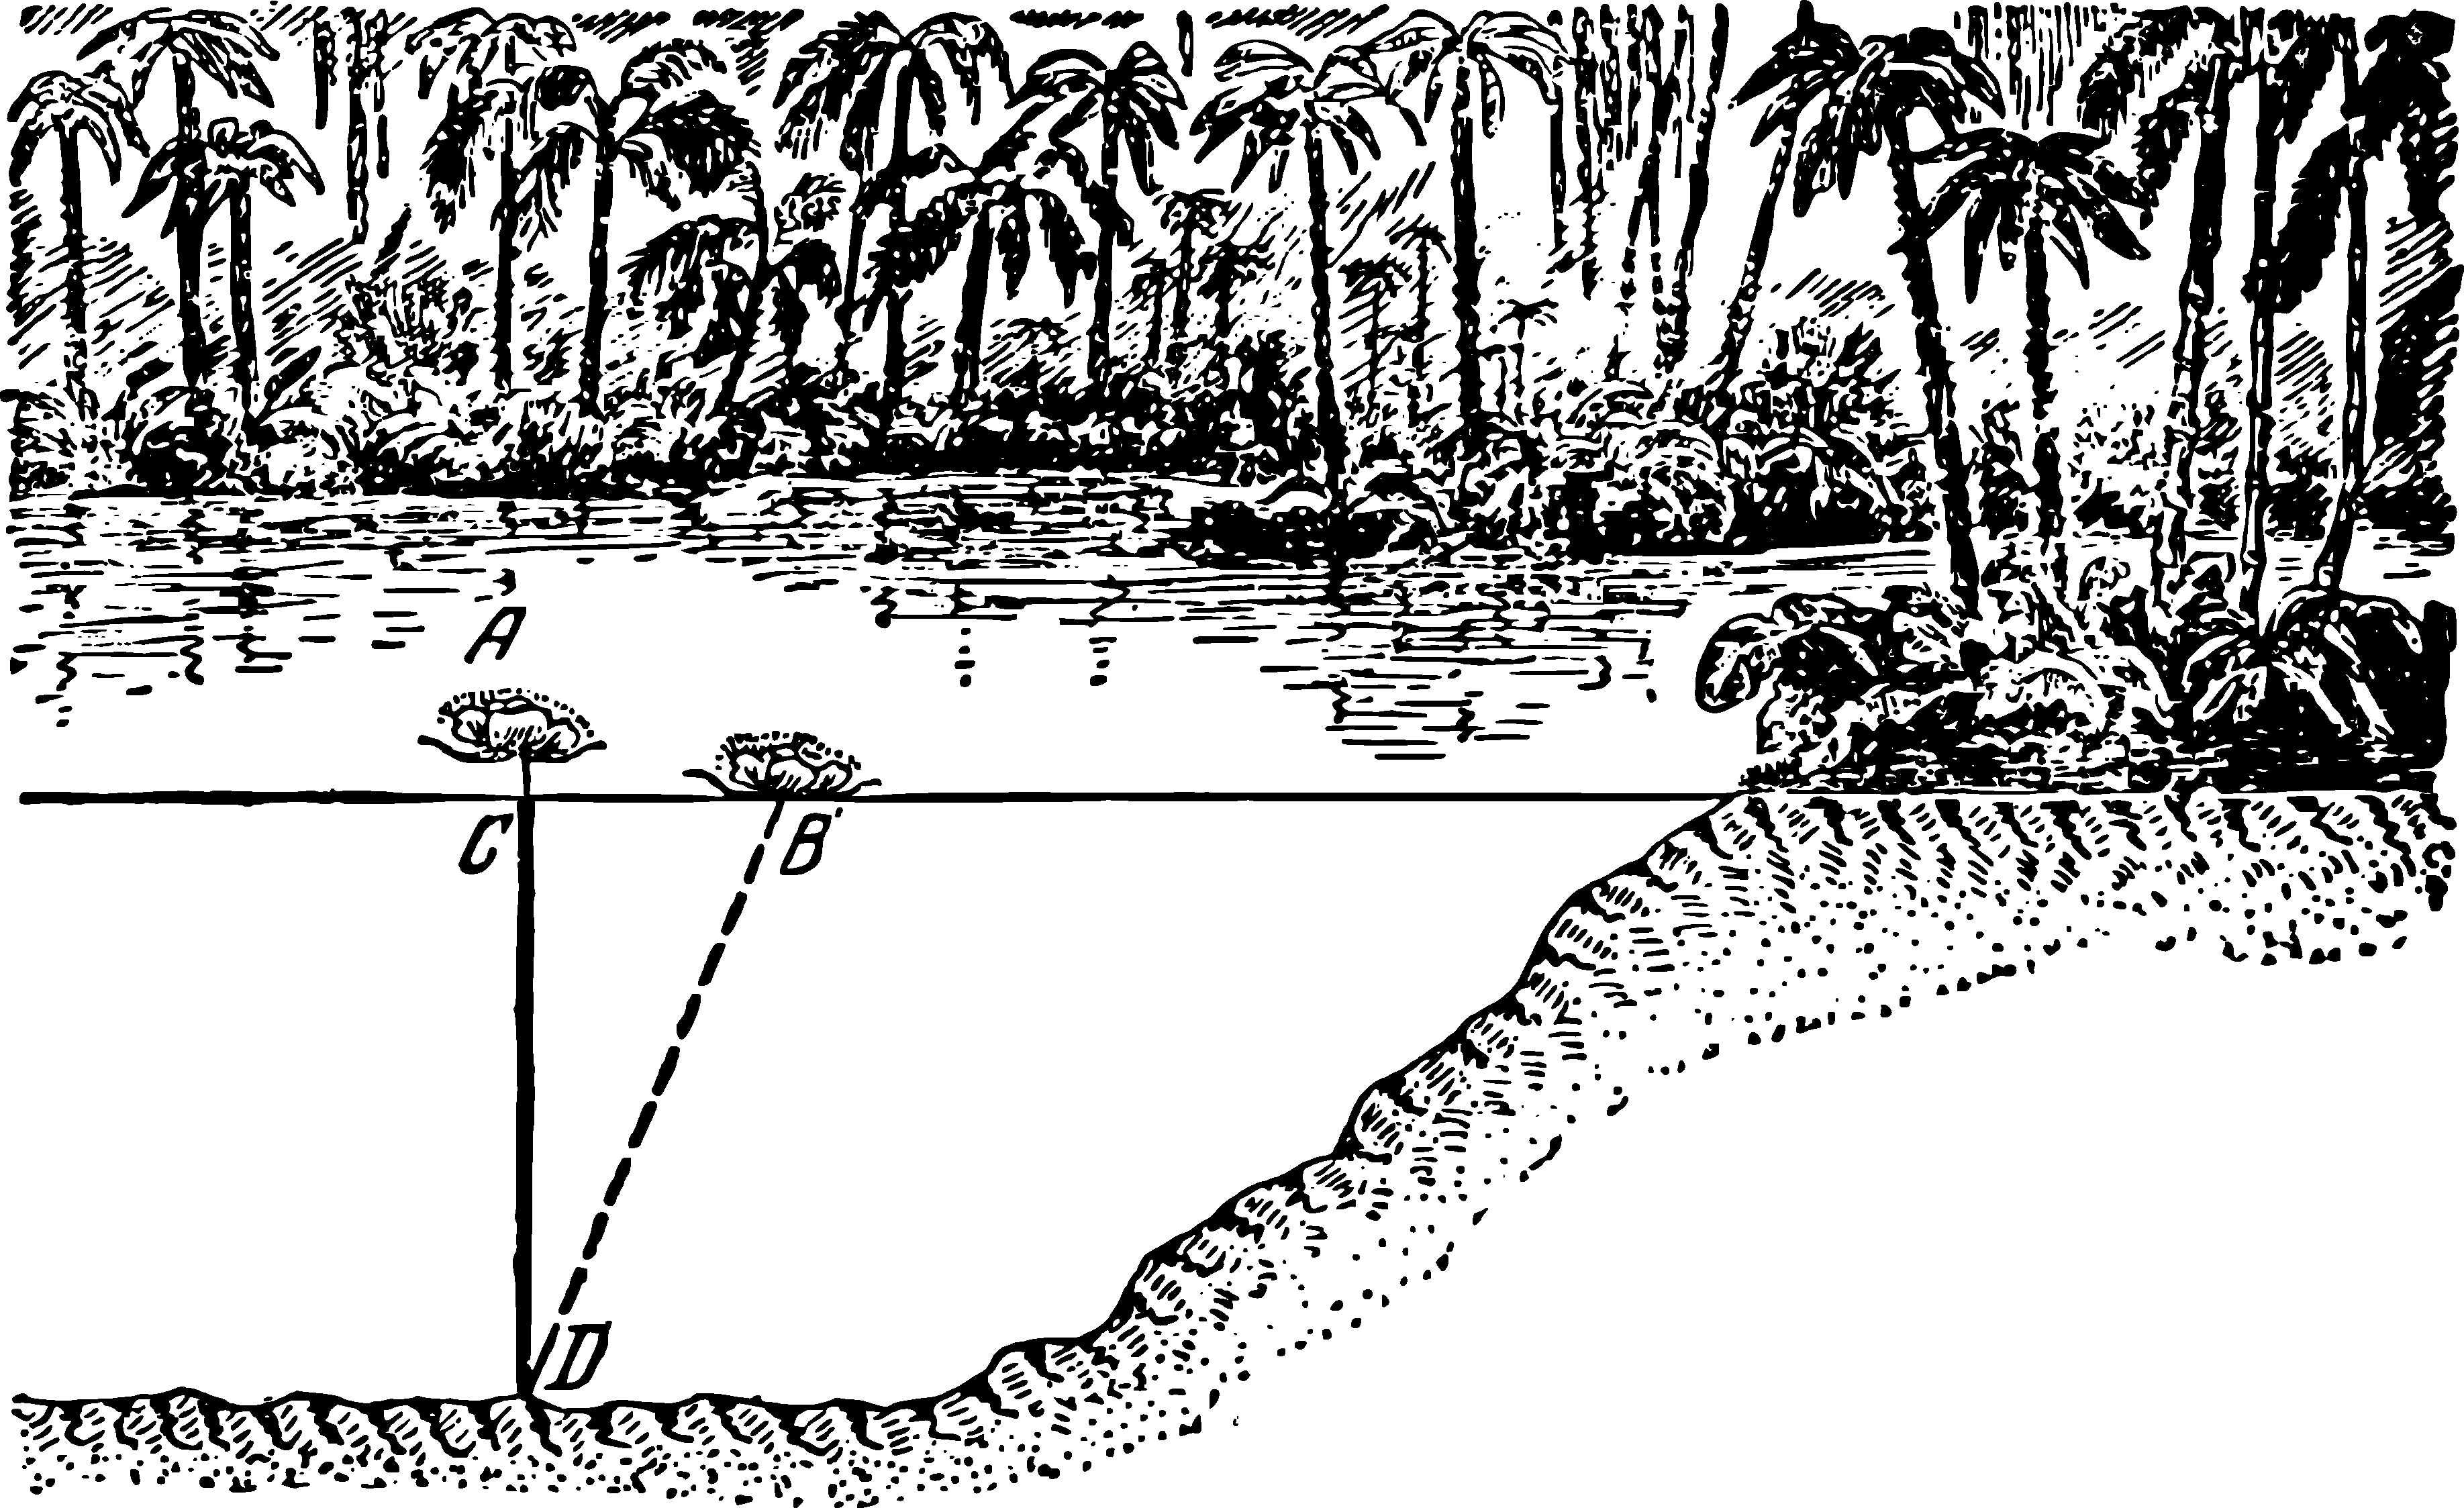
\includegraphics[width=\textwidth]{figures/ch-02/fig-053.pdf}
\sidecaption[][-2cm]{The Hindu problem of the lotus flower.\label{fig-053}}
\end{figure}



\ans Let's denote the depth of the pond $CD$ as \( x \) \figr{fig-053}. Then, according to the Pythagorean theorem, we have:
\begin{equation*}%
BD^{2} - x^{2} = BC^{2}.
\end{equation*}
Thus, 
\begin{equation*}%
x^{2} = \left( x + \frac{1}{2} \right)^{2} - 2^{2}.
\end{equation*}
From this, we get:
\begin{equation*}%
x^{2} = x^{2}  + x + \frac{1}{4} - 4 , \quad x = 3\,\frac{3}{4}
\end{equation*}

The depth is approximately $3\,\frac{3}{4}$ feet.

Near the riverbank or a shallow pond, you can find a water plant that will provide you with real material for a similar problem: without any tools, without even getting your hands wet, you can determine the depth of the water at that spot.



\section{Starry Sky in the River}
\label{sec-2.16}

The river also offers the geometer problems at night. Remember Gogol's description of the Dnieper: ``The stars burn and shine over the world and all are reflected in the Dnieper at once. The Dnieper holds them all in its dark womb: not one can escape from it, unless it goes out in the sky.'' Indeed, when standing on the bank of a wide river, it seems that the entire starry dome is reflected in the water mirror. But is it really so? Do all the stars ``surrender'' to the river?
\begin{marginfigure}[-1cm]%[h!]
\centering
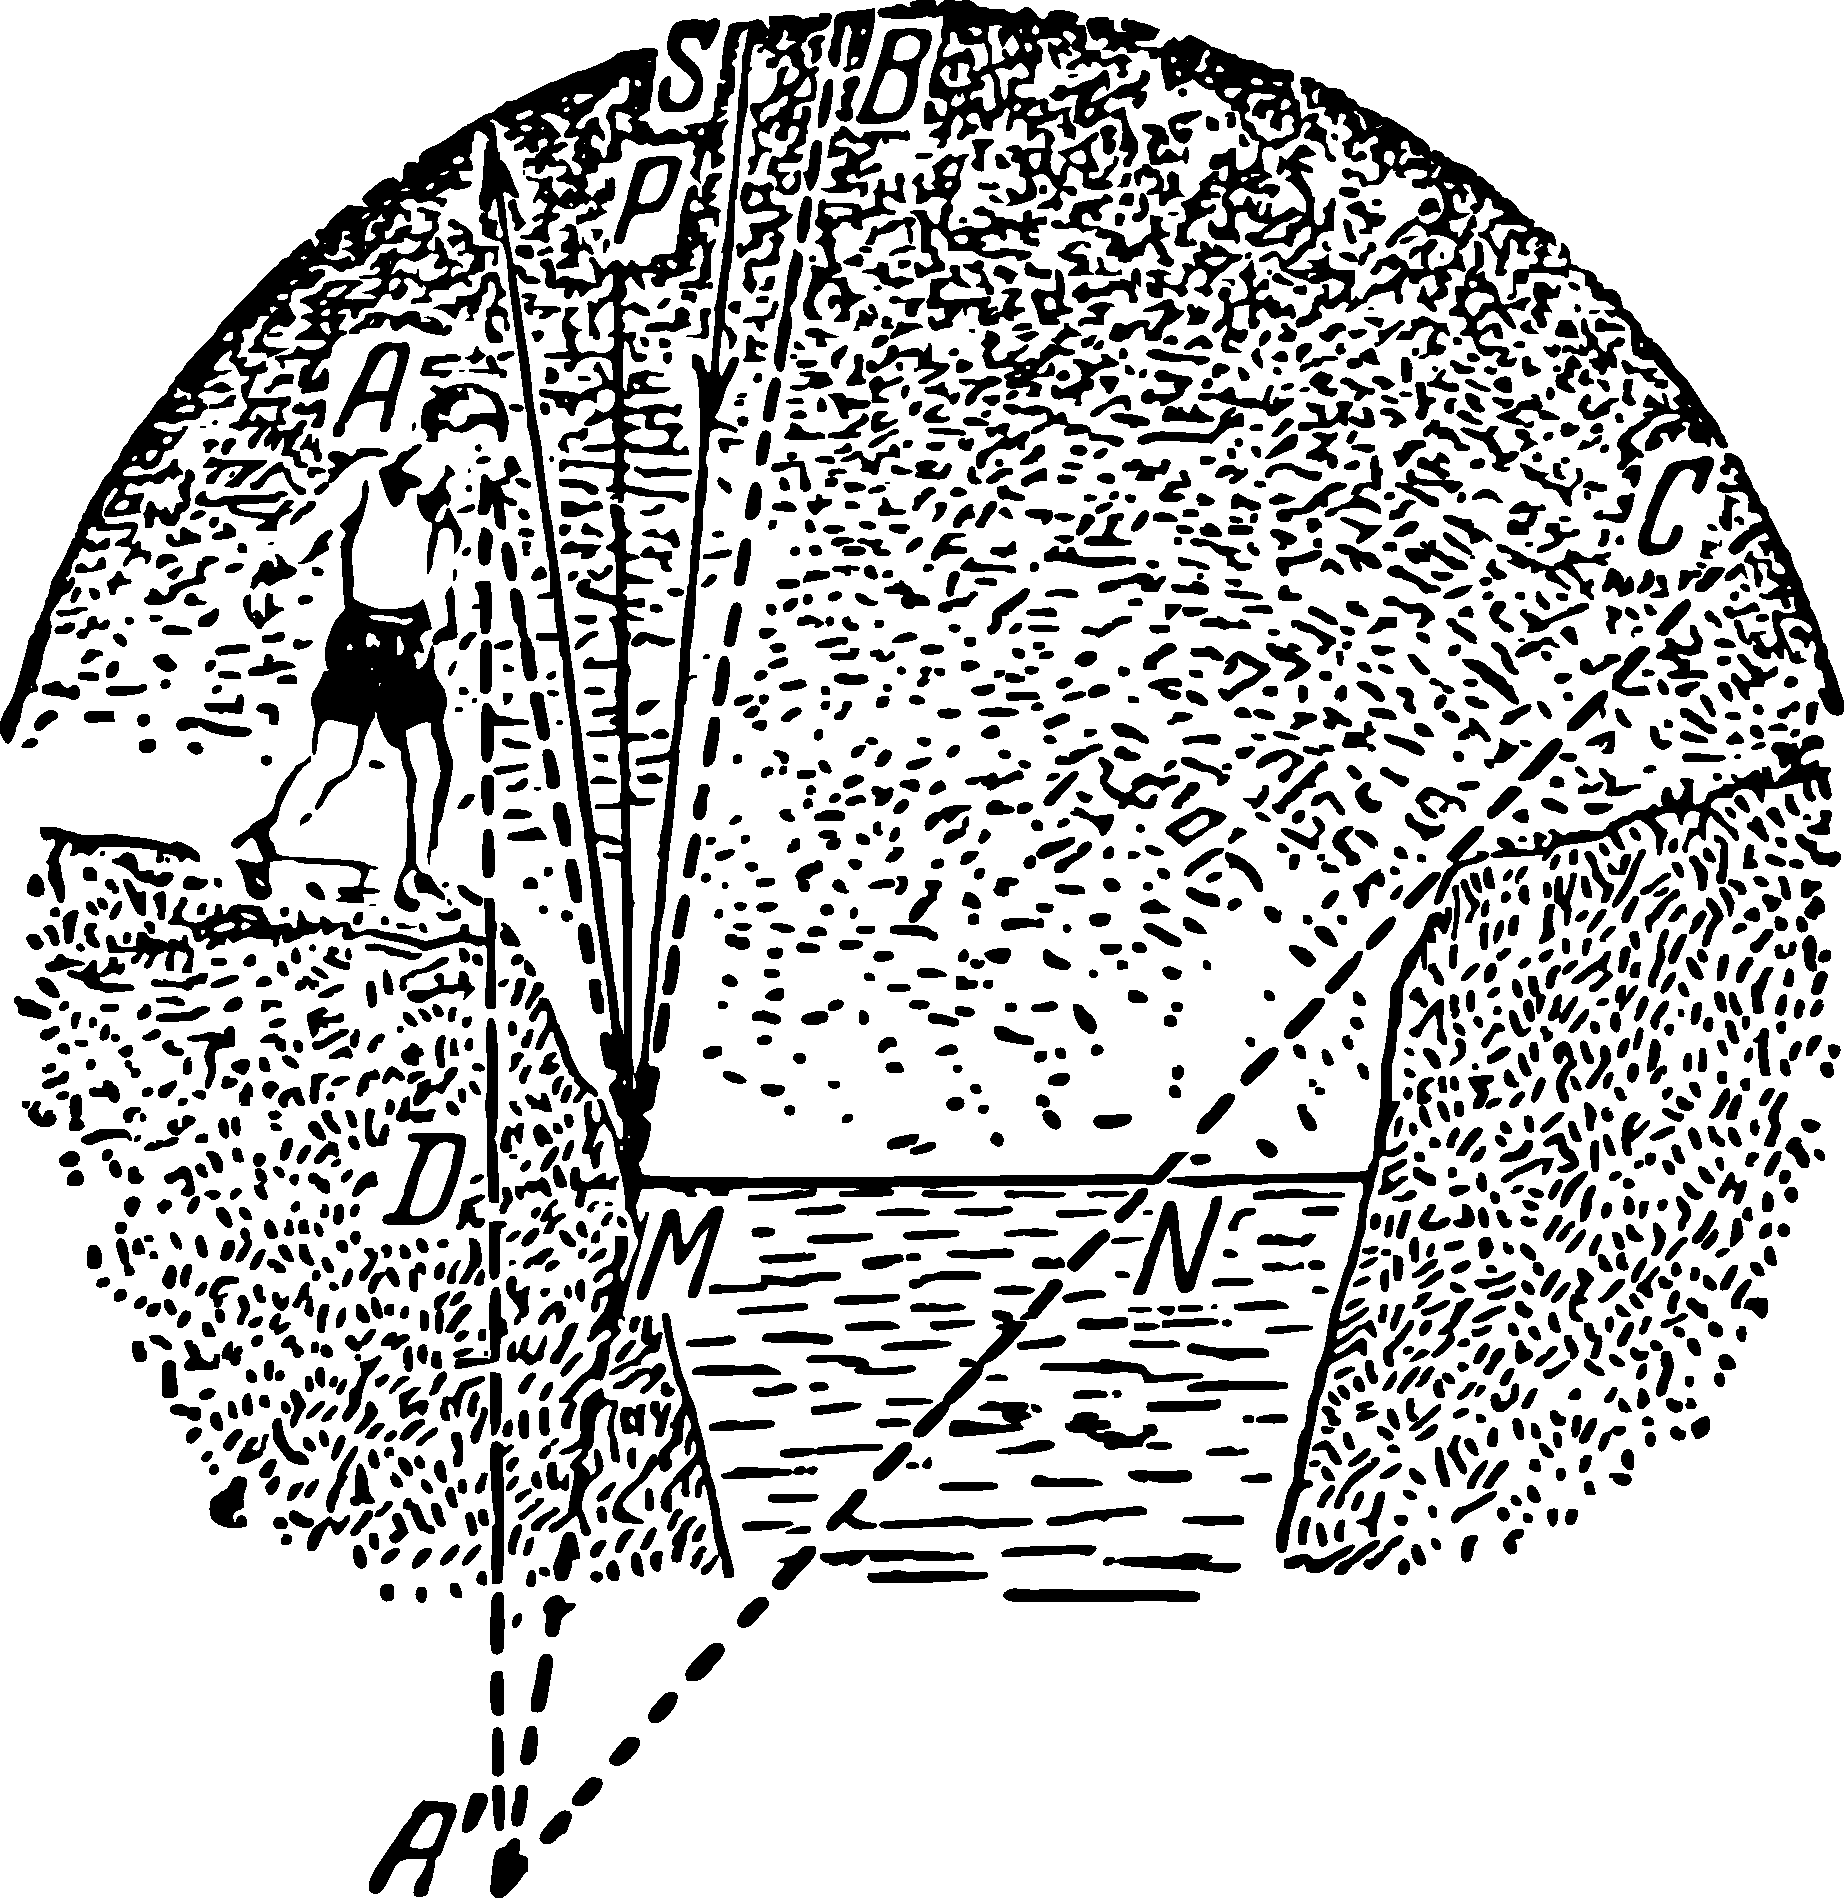
\includegraphics[width=1.\textwidth]{figures/ch-02/fig-054.pdf}
\sidecaption{Which part of the starry sky can be seen in the water channel of the river.\label{fig-054}}
\end{marginfigure}

Let's make a drawing (\figr{fig-054}): $A$ is the eye of the observer standing on the riverbank, at the edge of the cliff, $MN$ is the water surface. What stars can the observer see in the water from point $AD$? To answer this question, let's drop a perpendicular $AD$ from point $A$ to the line $MN$ and extend it to an equal distance to point $A'$. If the observer's eye were at $A'$, he could only see the part of the starry sky that fits inside angle $BA'C$. The actual observer's field of view from point $A$ is the same. Stars outside this angle are not visible to the observer; their reflected rays pass by his eyes.

\begin{marginfigure}[0cm]%[h!]
\centering
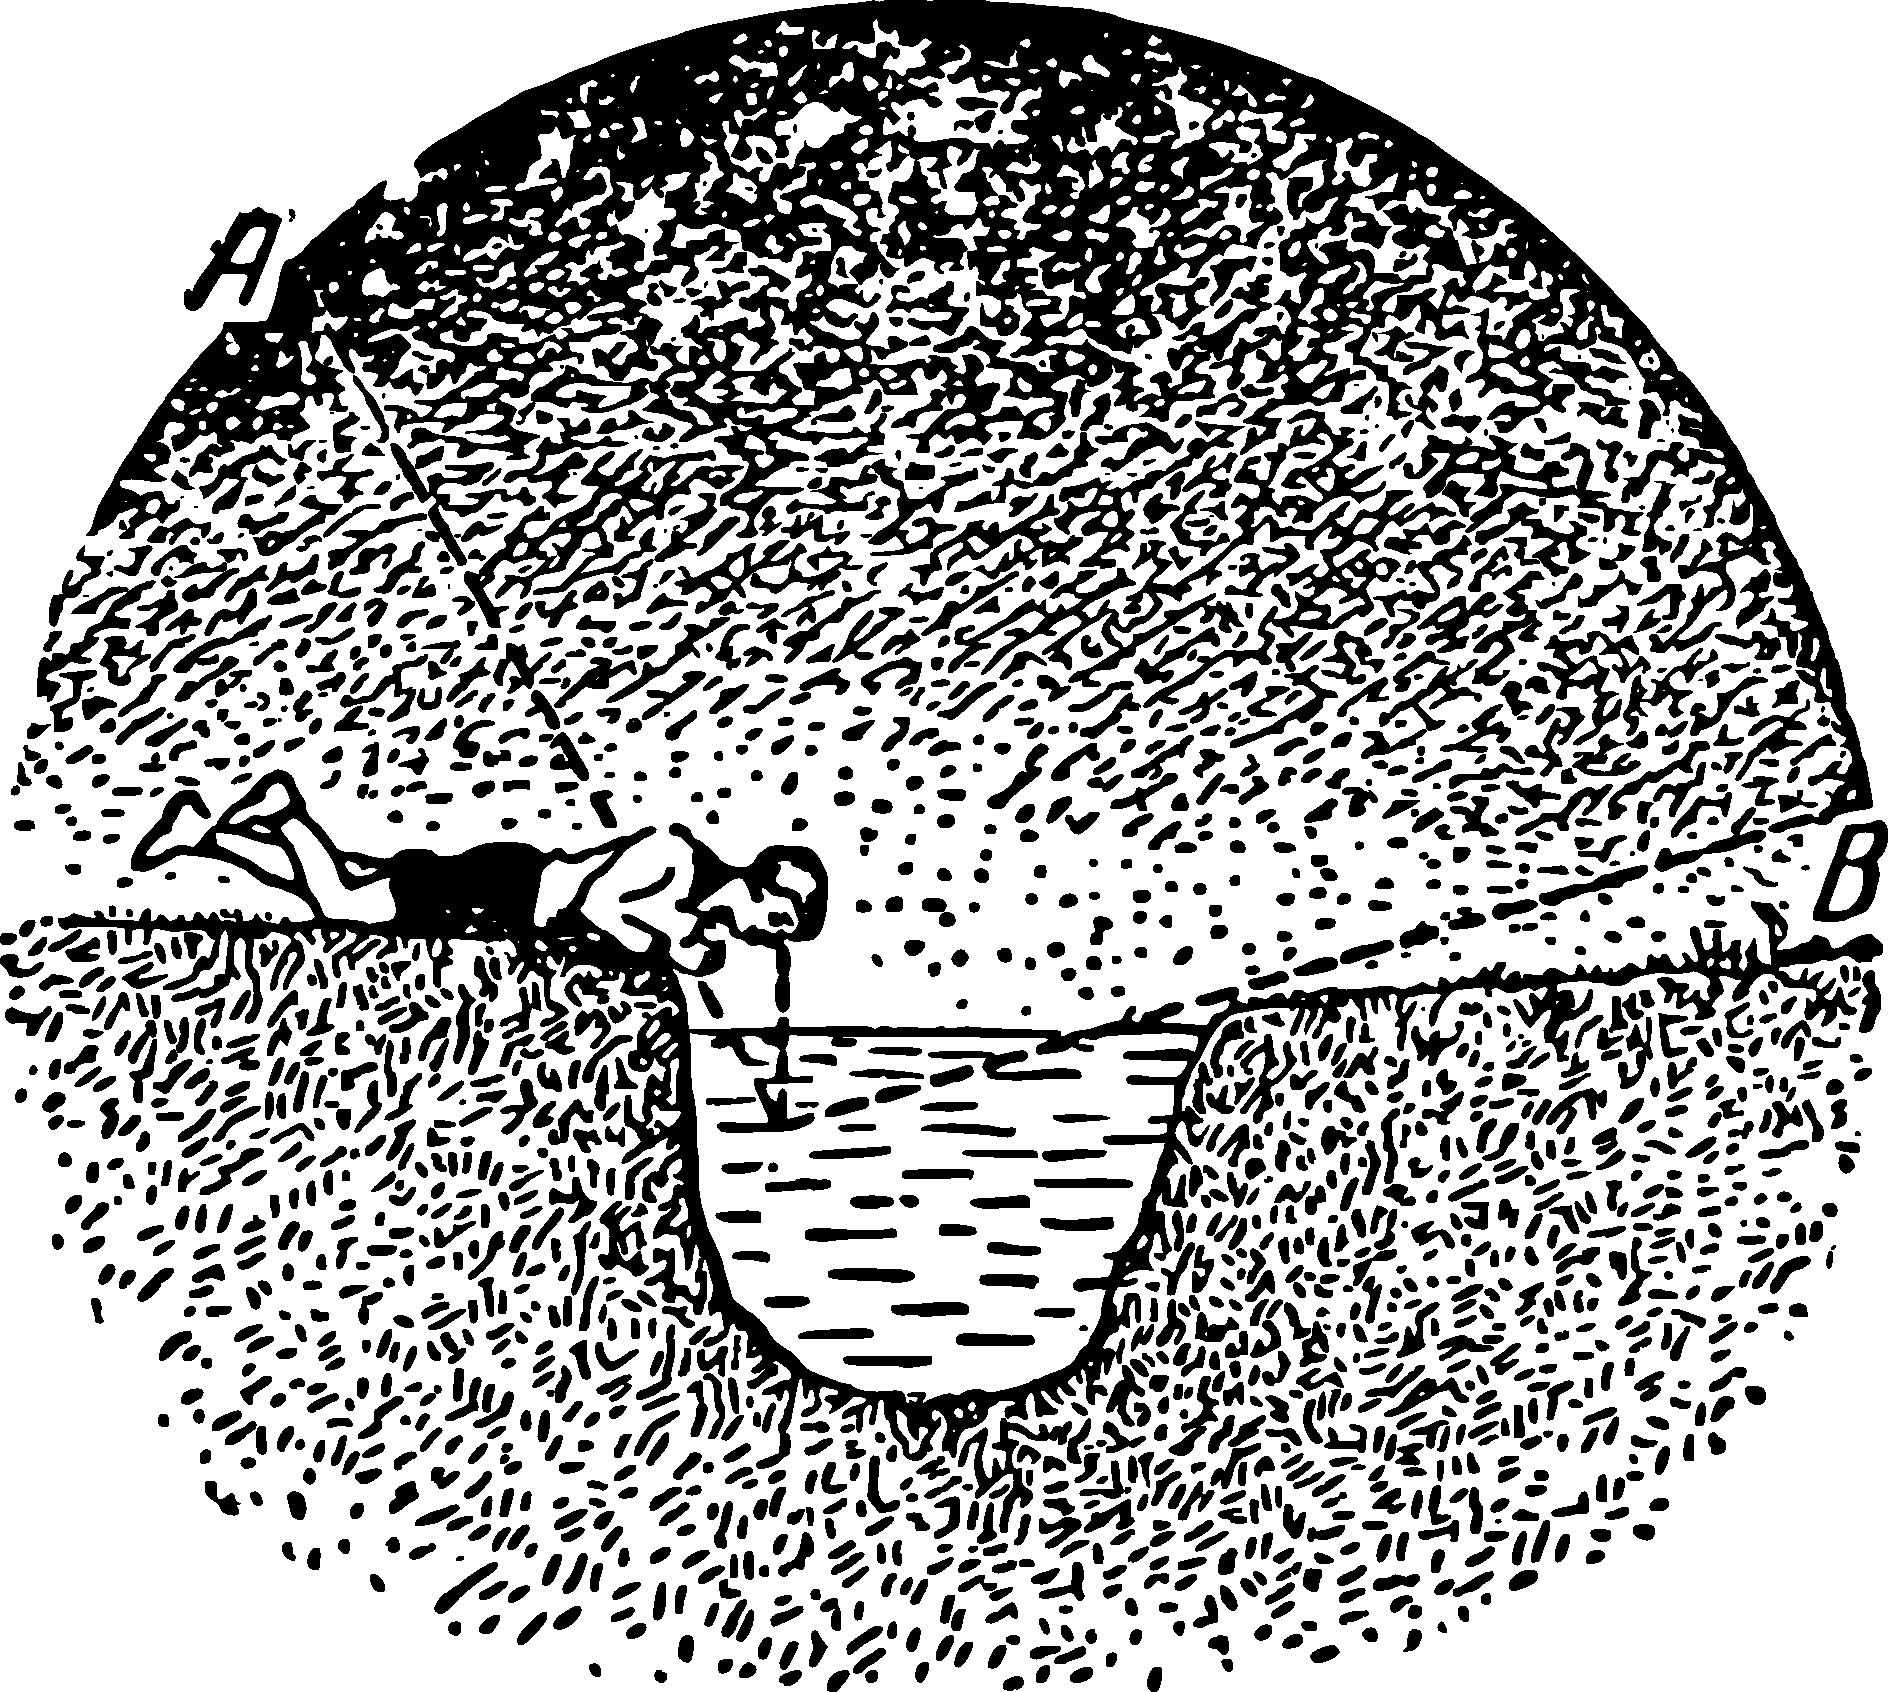
\includegraphics[width=1.\textwidth]{figures/ch-02/fig-055.pdf}
\sidecaption{In a narrow river with low banks, you can see more stars.\label{fig-055}}
\end{marginfigure}

How to make sure of this? How to prove that, for example, star $S$ lying outside angle $BA'C$ is not visible to our observer in the water mirror of the river? Let's follow its ray, falling close to the shore, to point $M$; it will reflect according to the laws of physics at an angle to perpendicular $MP$, which is equal to the angle of incidence $SMP$ and therefore less than angle $PMA$ (this is easy to prove based on the equality of triangles $ADM$ and $A'DM$); thus, the reflected ray must pass by $A$. Therefore, the rays of star $S$ reflected in points beyond point $M$ will also pass by the observer's eye.



Thus, Gogol's description contains exaggeration: not all stars are reflected in the Dnieper, or, at least, less than half of the starry sky. Even more interesting is that the extent of the reflected part of the sky does not prove that you are facing a wide river. In a narrow river with low banks, you can see almost half of the sky (which seems like a wide river) if you lean close to the water. You can easily verify this by constructing a field of view for such a case (\figr{fig-055}).


In a narrow river with low banks, you can see more stars.


\section{Path Across the River}
\label{sec-2.17}


\begin{marginfigure}%[1cm]%[h!]
\centering
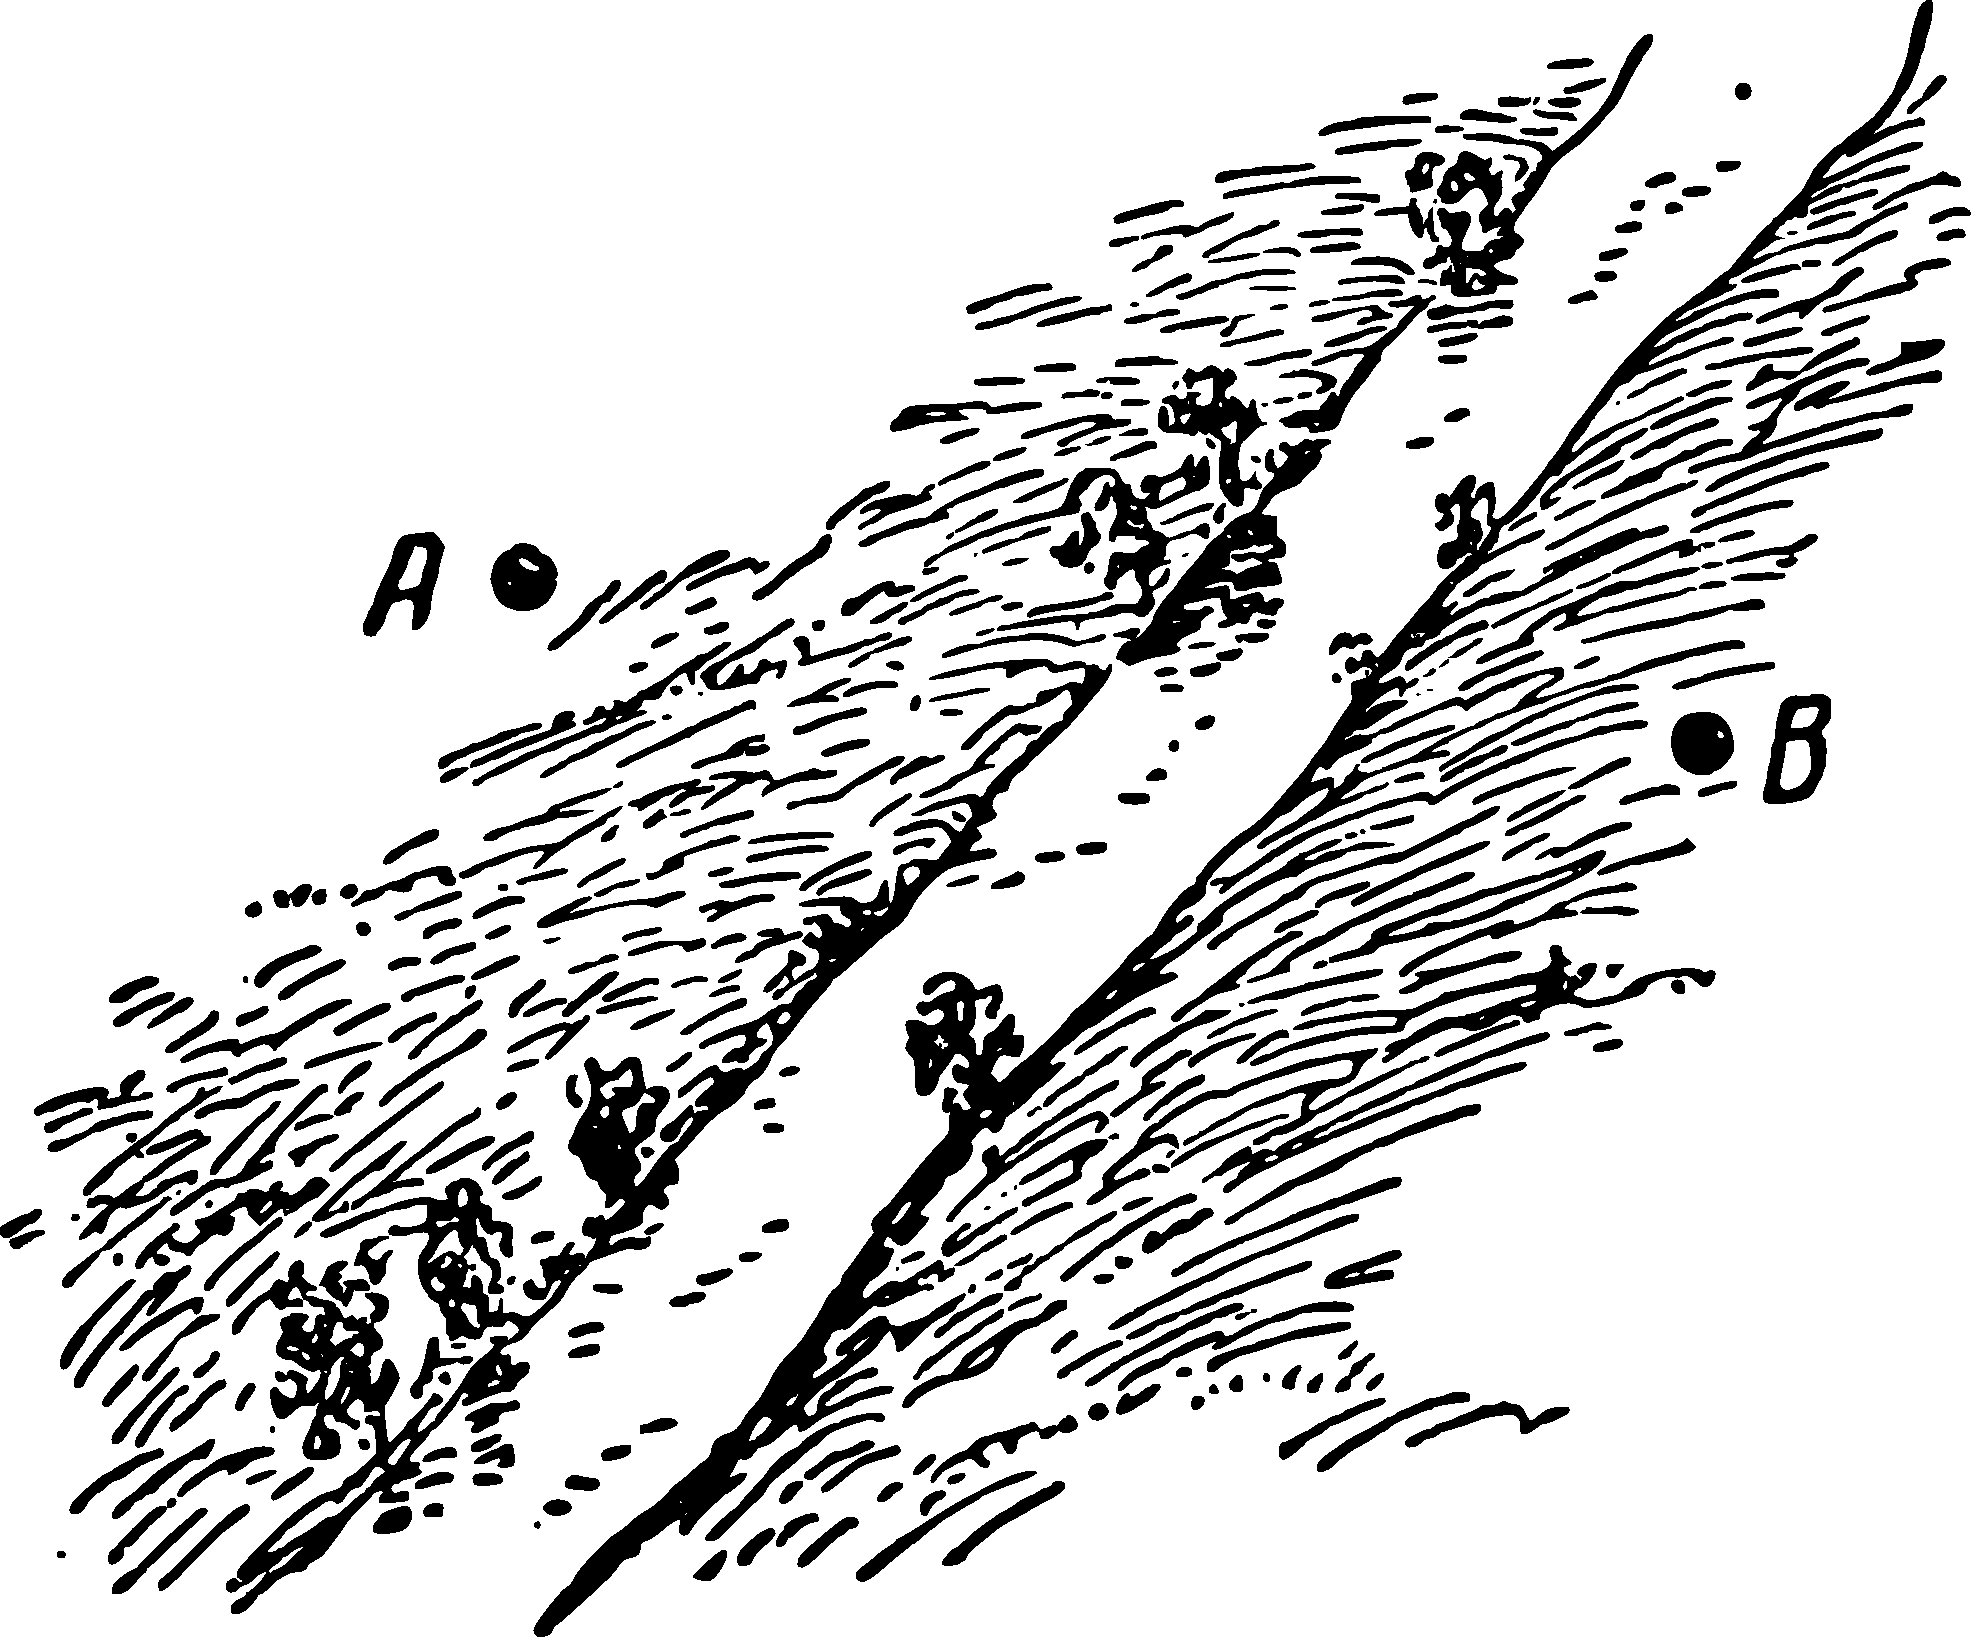
\includegraphics[width=1.\textwidth]{figures/ch-02/fig-056.pdf}
\sidecaption{Where can we build a bridge at right angles to the river banks so that the road from A to B is the shortest?\label{fig-056}}
\end{marginfigure}

\ques Between points $A$ and $B$, a river (or canal) flows with approximately parallel banks (\figr{fig-056}). It is necessary to construct a bridge across the river at right angles to its banks. Where should the bridge be placed to make the path from $A$ to $B$ the shortest?



\ans Drawing a straight line through point $A$ (\figr{fig-057}), perpendicular to the direction of the river, and marking off segment $AC$ equal to the width of the river from $A$, we connect $C$ to $B$. The bridge should be constructed at point $D$ to make the path from $A$ to $B$ the shortest.

\begin{figure}[h!]
\centering
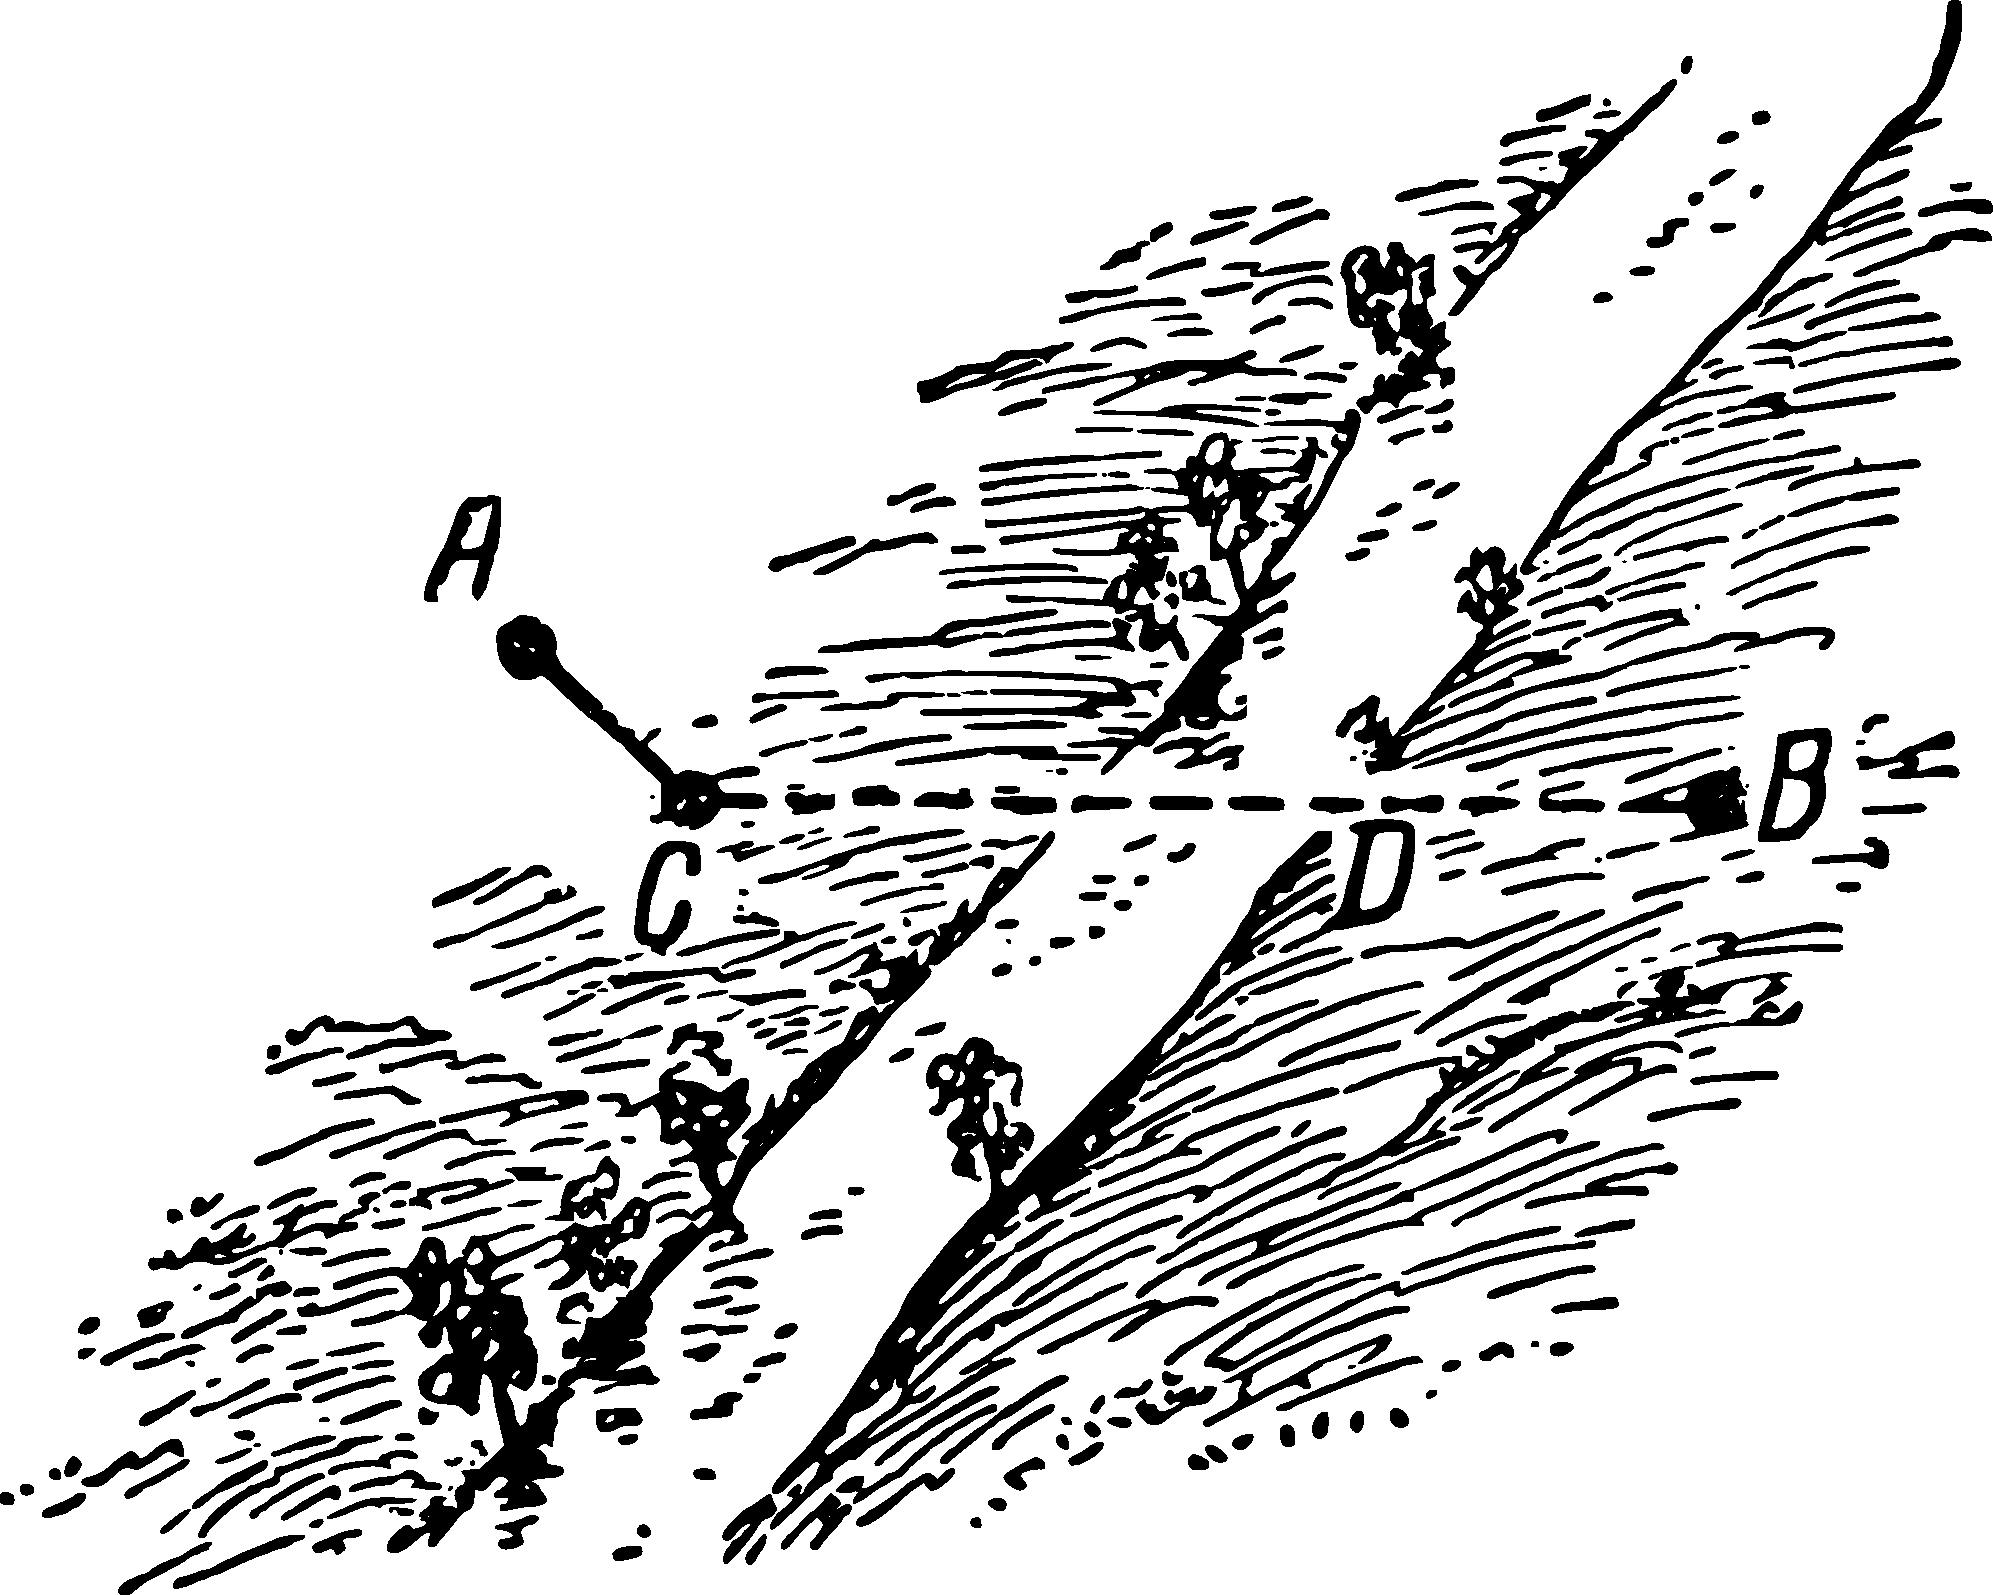
\includegraphics[width=0.6\textwidth]{figures/ch-02/fig-057.pdf}
\sidecaption{Choosing he location for building the bridge.\label{fig-057}}
\end{figure}

Indeed, by constructing bridge $DE$ (\figr{fig-058}) and connecting $E$ to $A$, we obtain the path $AEDB$, in which segment $AE$ is parallel to $CD$ ($AEDC$ is a parallelogram, as its opposite sides $AC$ and $ED$ are equal and parallel). Therefore, the length of path $AEDB$ equals the length of path $ACB$. It is easy to show that any other path is longer than this one. 

\begin{figure}[h!]
\centering
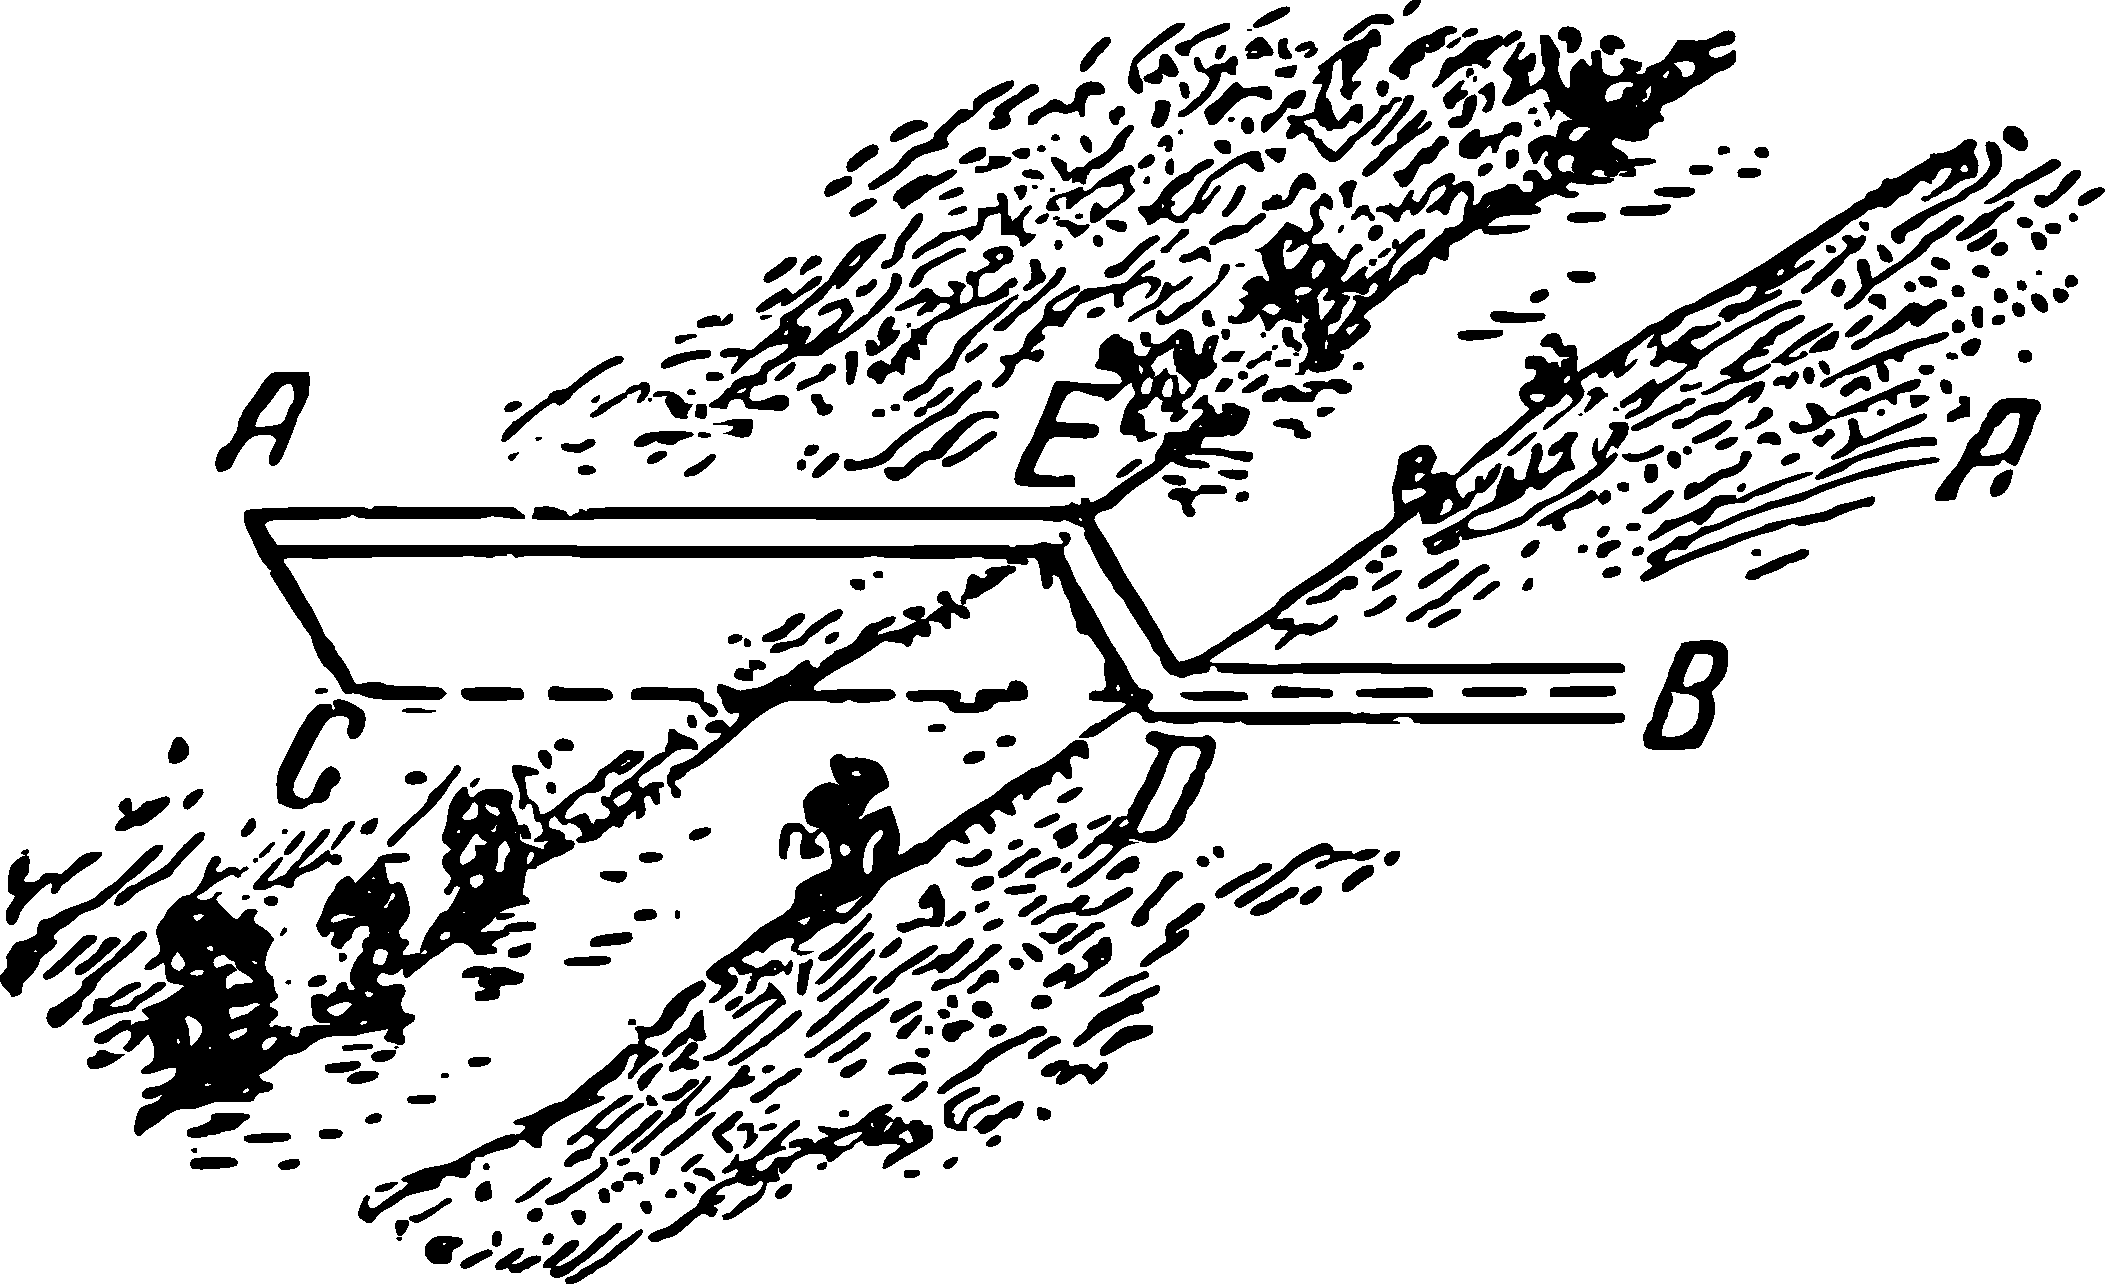
\includegraphics[width=0.6\textwidth]{figures/ch-02/fig-058.pdf}
\sidecaption{The bridge is built.\label{fig-058}}
\end{figure}


Suppose we suspect that some path $AMNB$ (\figr{fig-059}) is shorter than $AEDB$, i.e., shorter than $ACB$. Connecting $C$ to $N$, we see that $CN$ equals $AM$. Thus, path $AMNB = ACNB$. But $CNB$ is obviously greater than $CB$; therefore, $ACNB$ is greater than $ACB$, and consequently, greater than $AEDB$. Thus, the path $AMNB$ turns out to be not shorter but longer than the path $AEDB$. This reasoning applies to any position of the bridge that does not coincide with $ED$; in other words, the path $AEDB$ is indeed the shortest.

\begin{figure}[h!]
\centering
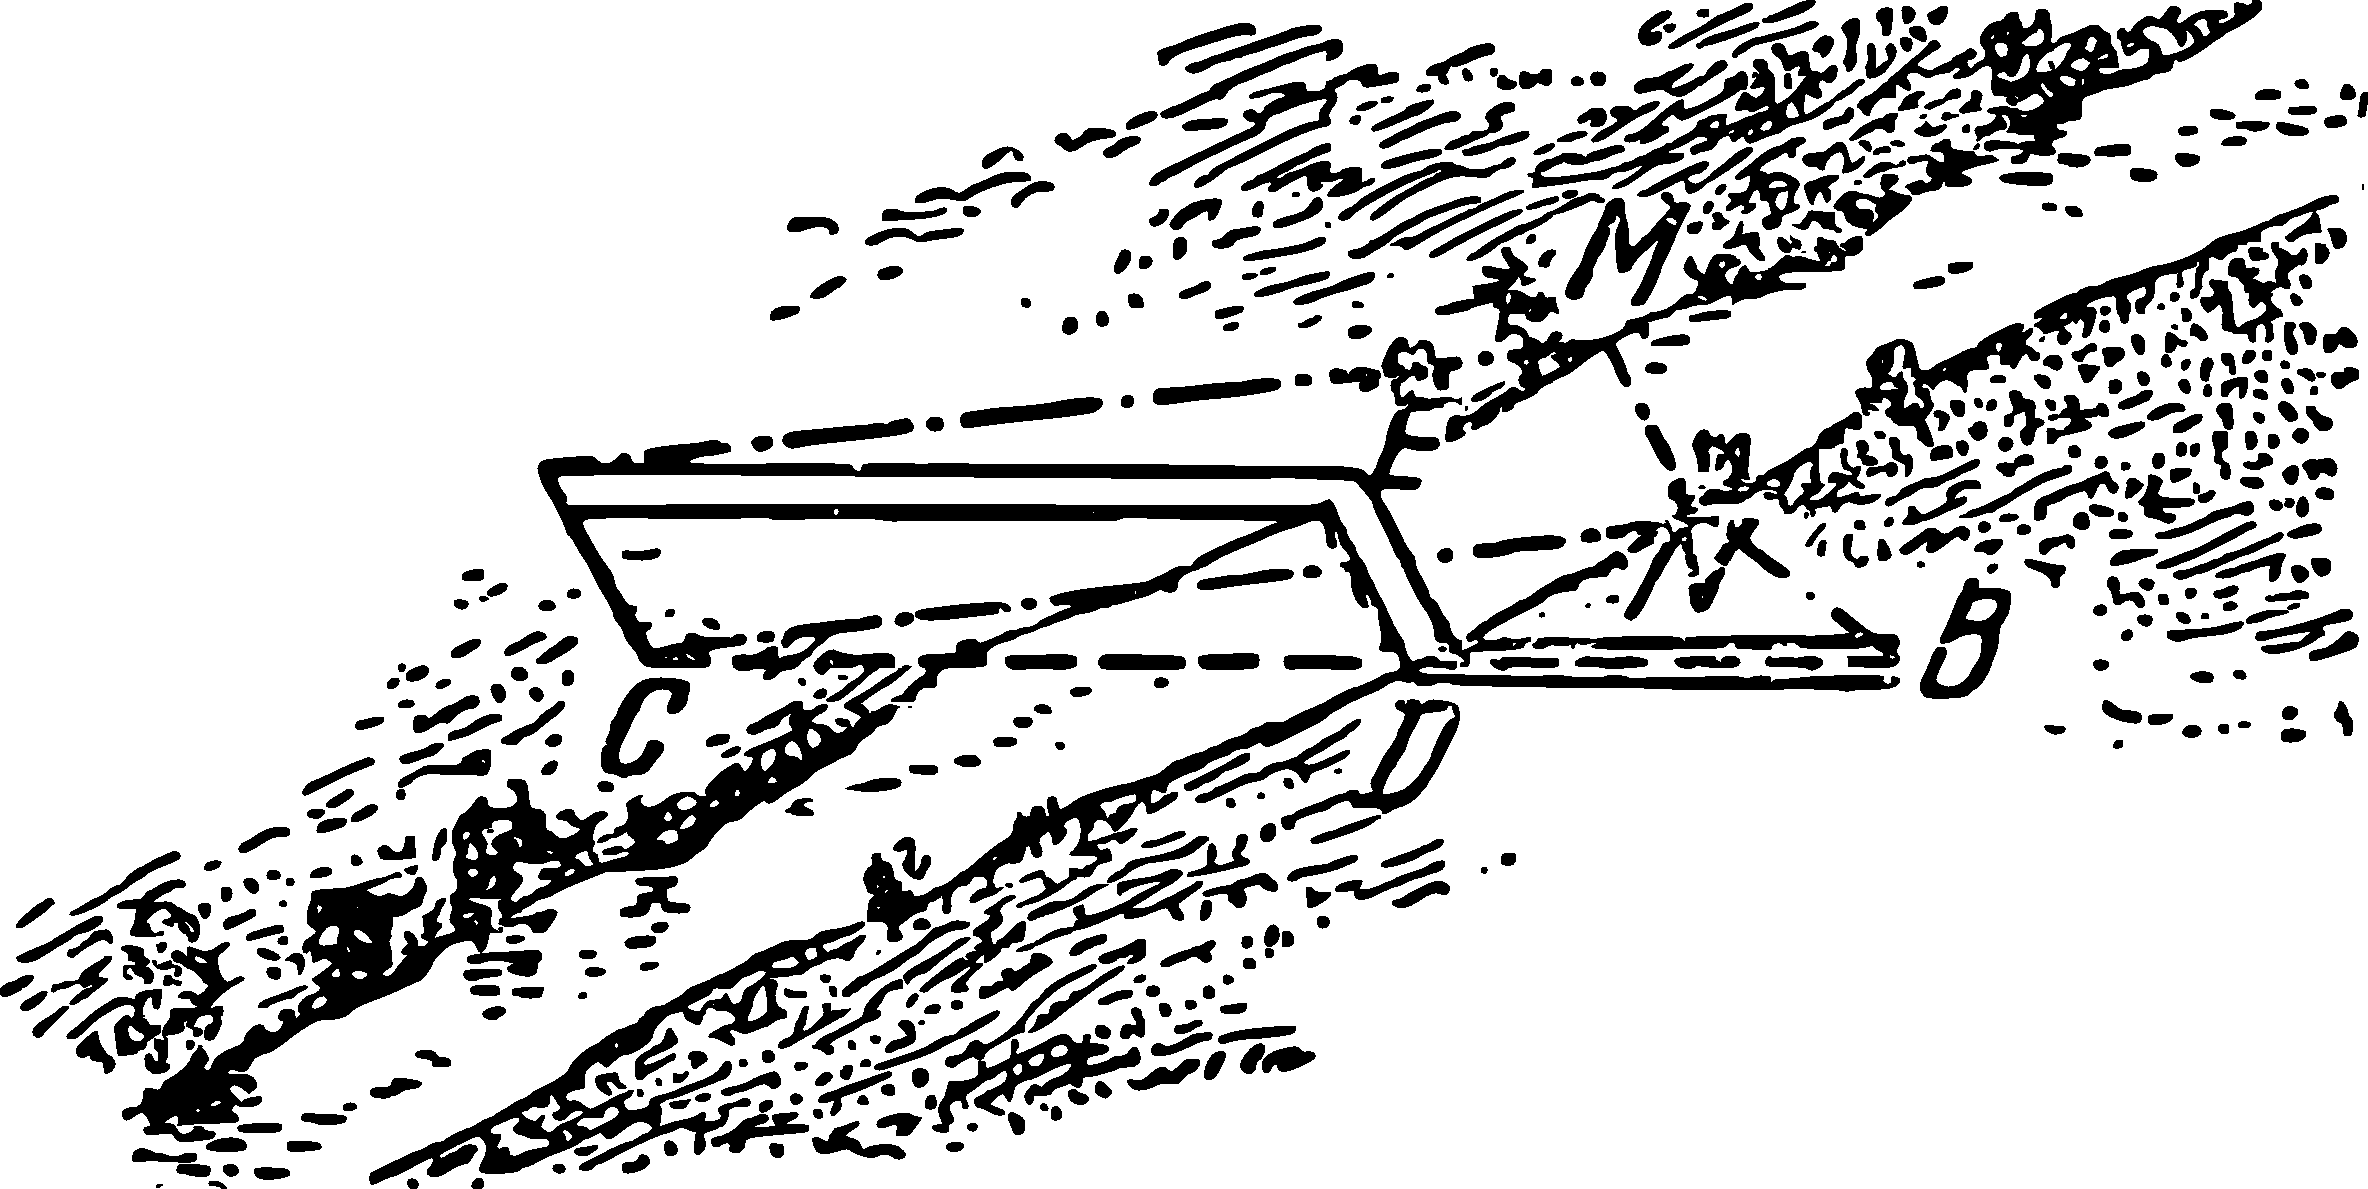
\includegraphics[width=0.65\textwidth]{figures/ch-02/fig-059.pdf}
\sidecaption{The $AEDB$ path is indeed the shortest.\label{fig-059}}
\end{figure}


\section{To Construct Two Bridges}
\label{sec-2.18}

\ques A more complex case may arise when it is necessary to find the shortest path from $A$ to $B$ across the river, which needs to be crossed twice at right angles to the banks (see \figr{fig-060}). In what places should bridges be built across the rivers?

\begin{figure}[h!]
\centering
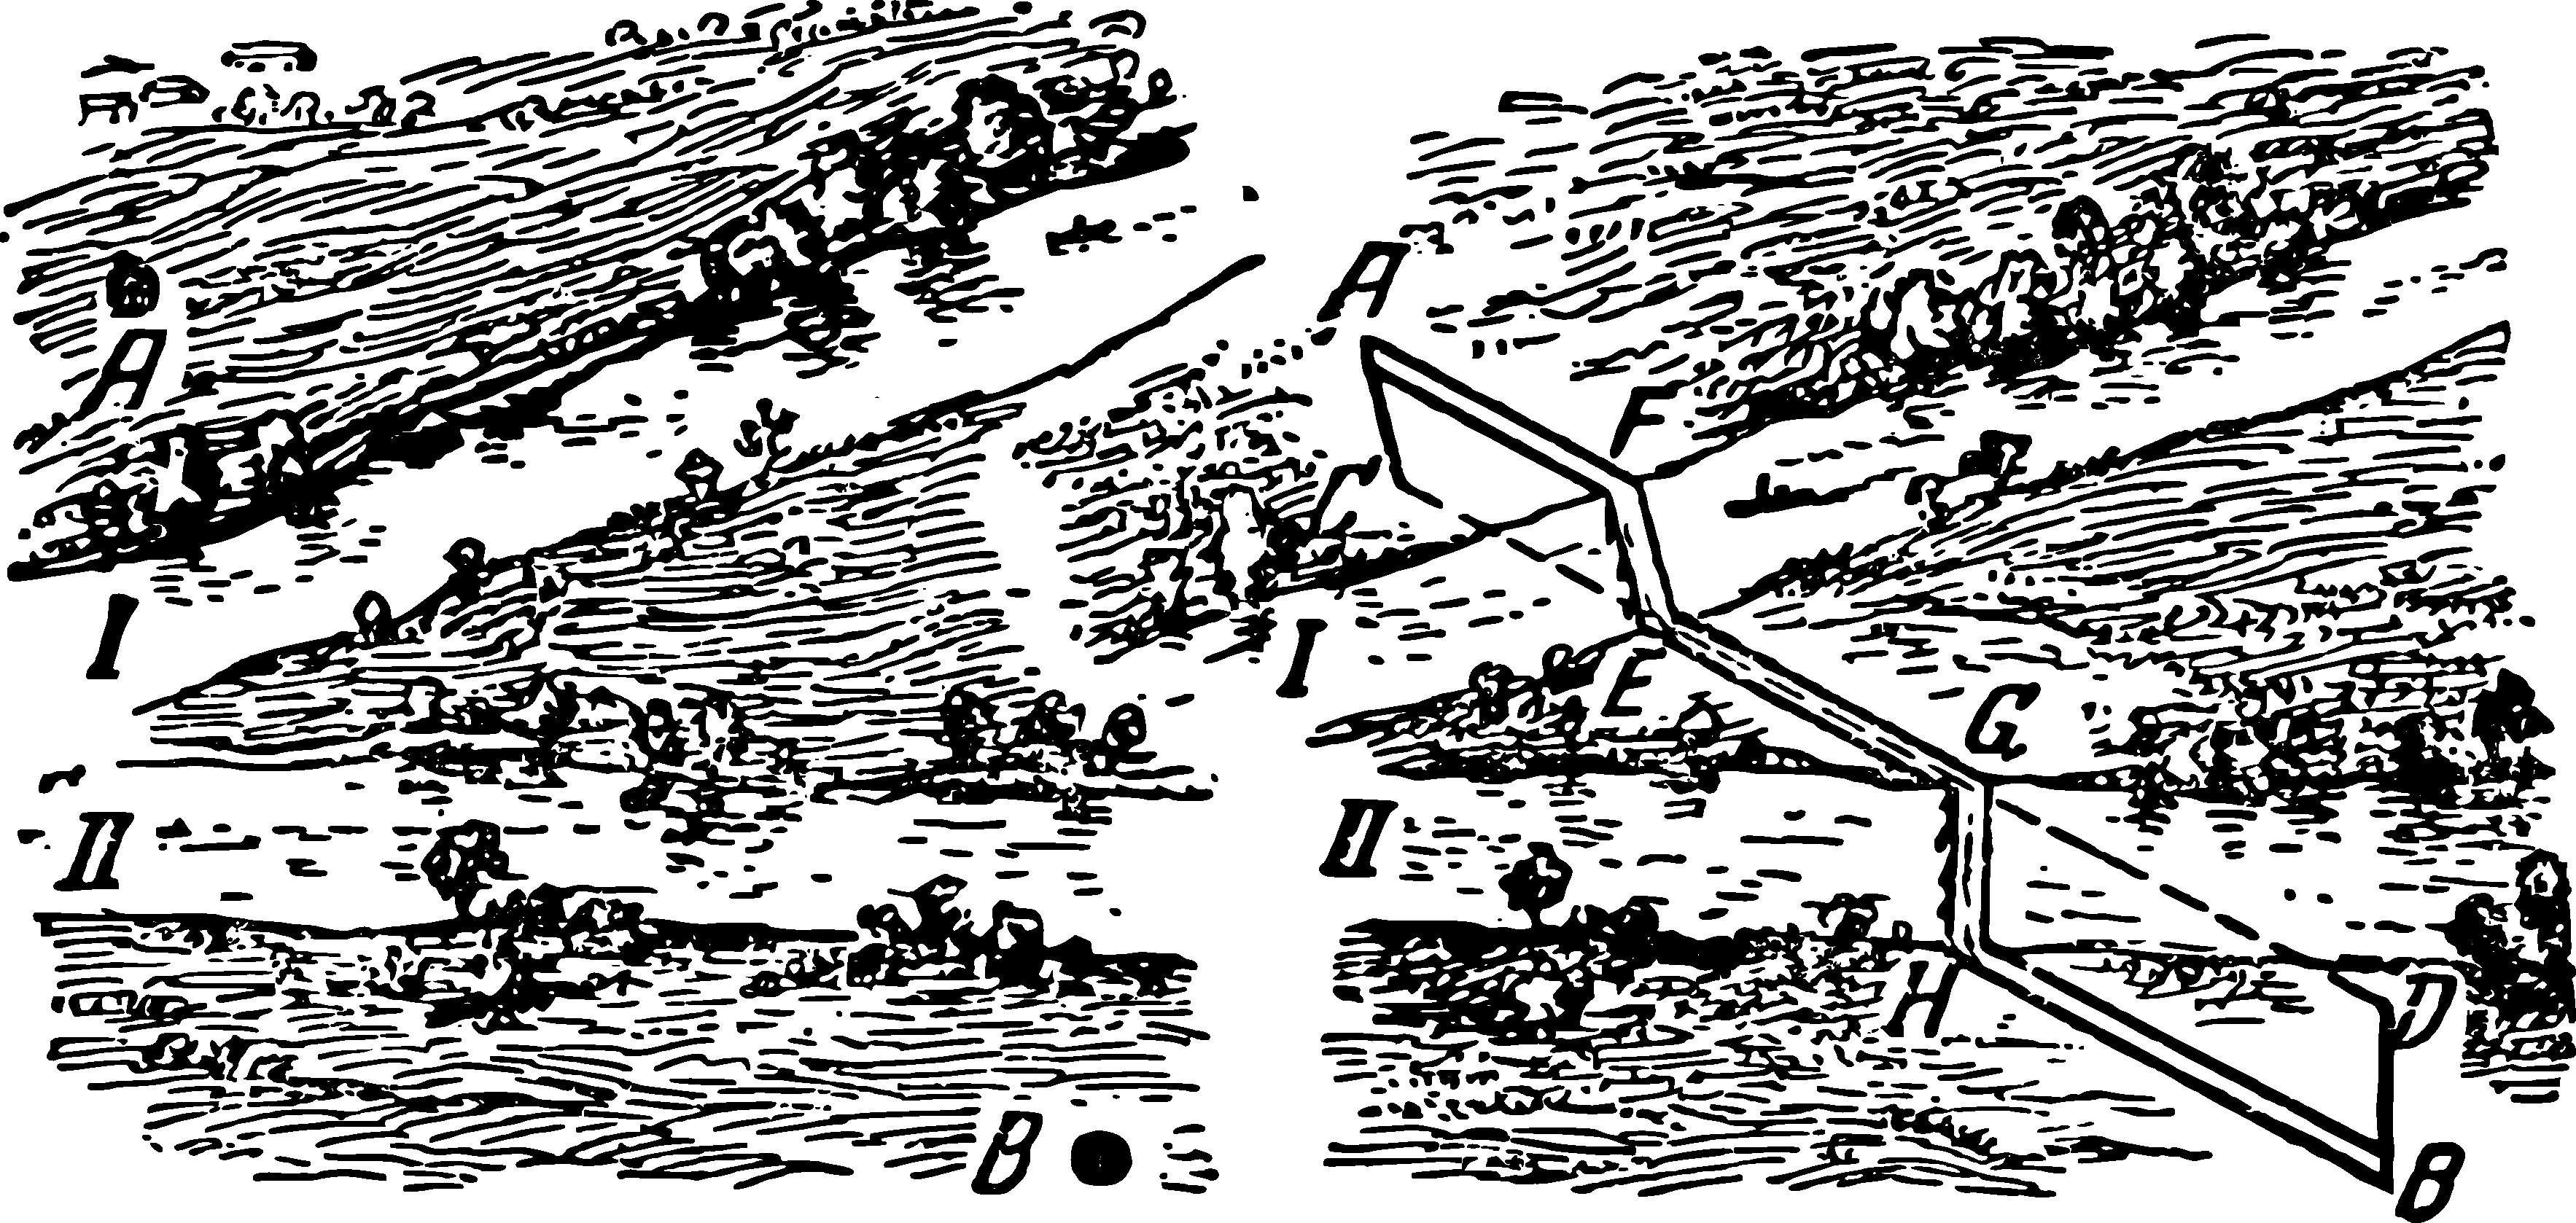
\includegraphics[width=0.9\textwidth]{figures/ch-02/fig-060.pdf}
\sidecaption{Two bridges are built.\label{fig-060}}
\end{figure}

\ans It is necessary to draw a line segment $AC$ from point $A$ (to the right in the \figr{fig-060}), equal to the width of the river at point $C$, and perpendicular to its banks. From point $B$, draw a line segment $BD$ equal to the width of the river at point $D$, also perpendicular to the banks. Connect points $C$ and $D$ with a straight line. Build bridge $EF$ at point $E$ and bridge $GH$ at point $G$. The path $AFEGHB$ is the sought shortest path from $A$ to $B$.


The reader will, of course, understand this if reasoning in this case is conducted in the same way as we reasoned in the previous problem.




\begin{center}
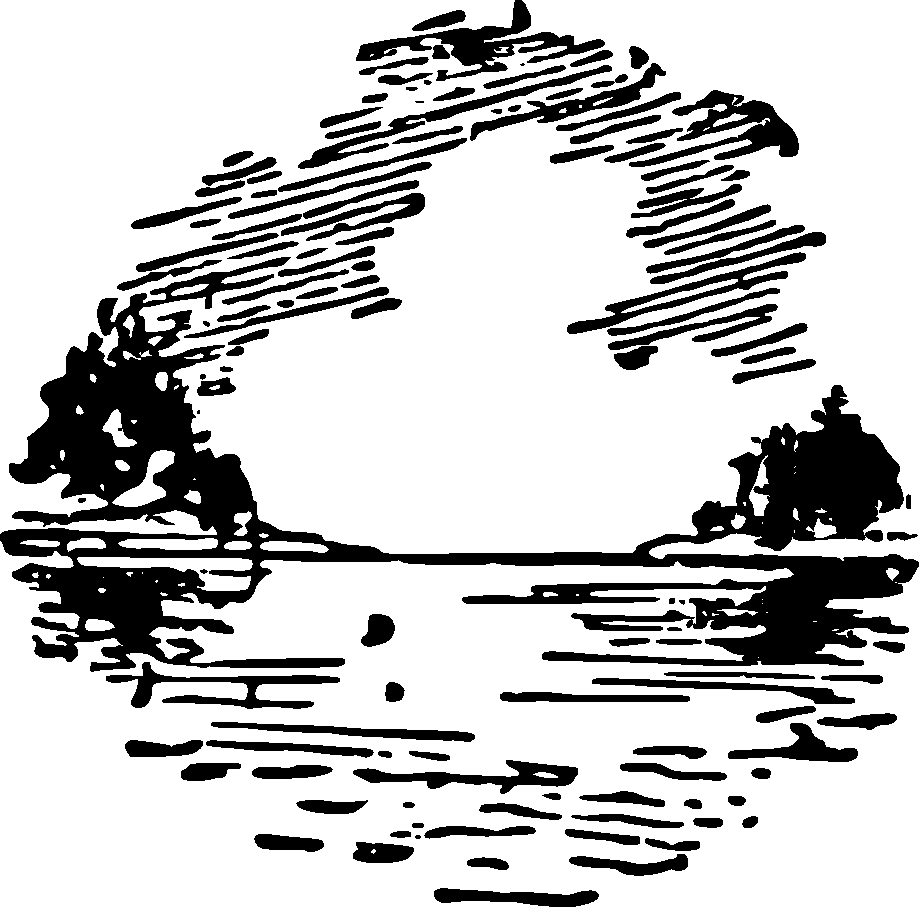
\includegraphics[width=0.3\textwidth]{figures/ch-02/fig-ch-02-tail.pdf}
\end{center}


















